\documentclass[11pt,a4paper]{article}

\usepackage{amsfonts,amssymb,amsmath}
\usepackage[margin=1in]{geometry}
\usepackage[none]{hyphenat}
\usepackage{graphicx}
\usepackage{fancyhdr}
\usepackage{float}
\usepackage{color}
\usepackage{xcolor}
\usepackage{tikz}
\usepackage{polynom}
\usepackage{bigints}
\usepackage{esint}
\usepackage[nottoc,notlot,notlof]{tocbibind}

\usetikzlibrary{quotes,angles,graphs,patterns,fadings,arrows.meta,shapes,trees,bending}

% grad, div and curl are operator NAMES. Set as bare letters in maths they come
% out italic, so "grad" reads as the product g.r.a.d - the same defect as a bare
% \cos. These give them upright type and the correct spacing.
\DeclareMathOperator{\grad}{grad}
\DeclareMathOperator{\dive}{div}
\DeclareMathOperator{\curl}{curl}

\parindent 0ex
\setlength{\parskip}{0.55\baselineskip}
% Displays carry their own skips; with a non-zero \parskip on top of them,
% consecutive displays drift apart. Tighten them so a derivation reads as one
% argument rather than as a column of disconnected formulae.
\setlength{\abovedisplayskip}{0.5\baselineskip}
\setlength{\belowdisplayskip}{0.5\baselineskip}
\setlength{\abovedisplayshortskip}{0.25\baselineskip}
\setlength{\belowdisplayshortskip}{0.25\baselineskip}

\pagestyle{fancy}
\fancyfoot[C]{\thepage}
\fancyhead{}
\fancyhead[R]{\rightmark}
\renewcommand{\headrulewidth}{0pt}

% Theorem environments. The source declared none: its 125 examples, 91
% solutions, 21 definitions and 30 theorems were set as red bold text with the
% number typed by hand, so LaTeX numbered nothing and inserting an example meant
% renumbering the rest of the subsection.
\usepackage{amsthm}
\theoremstyle{definition}
% One shared counter running section.subsection.n, as in the other courses here.
\newtheorem{thm}{Theorem}[subsection]
\newtheorem{defn}[thm]{Definition}
\newtheorem{exa}[thm]{Example}
\newtheorem{prop}[thm]{Proposition}
\newtheorem{coro}[thm]{Corollary}
\newtheorem{lem}[thm]{Lemma}
\newtheorem{result}[thm]{Result}
\newtheorem{exe}[thm]{Exercise}
\newtheorem*{note}{Note}
\newtheorem*{remark}{Remark}
\newtheorem{problemx}{Problem}[subsection]
\newenvironment{problem}{\begin{problemx}}{\end{problemx}}
\newenvironment{solution}
  {\renewcommand{\qedsymbol}{}\begin{proof}[\textit{Solution}.]}
  {\end{proof}}
\usepackage{enumitem}
% This source uses \multirow in its Cayley tables and \cancel in its coset
% arguments; neither is in the shared preamble.
\usepackage{multirow}
\usepackage{cancel}
% A heading that is legal inside a theorem body, a list or a float, where
% \subsubsection is not. Same weight as \subsubsection* so the two read alike.
\newcommand{\subhead}[1]{%
  \par\medskip\noindent\textbf{#1}\par\nobreak\smallskip}

\begin{document}
% Title page depersonalised for the web, as with every other course here.
% The identity kept below is Lagrange's theorem, which is the first result in
% the subject that could not have been guessed from the definitions.
\begin{titlepage}
\thispagestyle{empty}
\begin{center}
\vspace*{3cm}
{\Huge\bfseries Abstract Algebra}\\[1.2cm]
{\large Lecture Notes}\\[2.5cm]
\line(1,0){300}\\[1.5cm]
$$\left|G\right| = \left[G:H\right]\,\left|H\right|$$
\end{center}
\end{titlepage}

\tableofcontents
\thispagestyle{empty}
\clearpage
\setcounter{page}{1}

















\section{GROUP}

\textbf{What is A GROUP?}\\



\begin{defn}
A group is a set $G$ together with an operation $`*$' on G. Satisfying the following conditions:
\begin{enumerate}
\item $a*(b*c) = (a*b)*c\,\, \forall a\, , \, , \, c\,\in G\,\hspace{0.3cm} -$Associativity
\item $\exists\, e\in G\ni \, a*e = e*a = a, \,\, \forall\, a\in G\,\hspace{0.3cm} -$Identity
\item $\forall a\in G\, ,\, \exists\, b\ni \, a*b = b*a = e\, \hspace{0.3cm}-$Inverse ($b$ is called the inverse of $a$).\\\\
\end{enumerate}
\end{defn}




\textbf{Examples}
\begin{enumerate}
\item The set of even integers with addition $\hspace{0.5cm}2\mathbb{Z} = \{0\, ,\, \pm 2\, , \, \pm 4\, , \cdots\cdots\}\,\, (2\mathbb{Z}\, ,\, +)$
\begin{enumerate}
       \item[(i)] $2r + (2s + 2t) = (2r + 2s) + 2t.\hspace{0.3cm}$ holds
       \item[(ii)] $a+ 0 = 0 + a = a\hspace{0.3cm}$ holds $\, 0\in 2\mathbb{Z}=$ (even numbers)
       \item[(iii)] $a + (-a) = (-a) + a  = a\hspace{0.3cm}$ holds
\end{enumerate}
$\therefore\,\, $ Even integers with addition form a group.\\



\item $\{0\}$ with addition is a group. Since $\, \, \big(\{0\}\, , \, +\big)$
\begin{enumerate}
       \item[(i)] $0 + (0 + 0) = (0 + 0) + 0 = 0$
       \item[(ii)] $ 0 + 0 = 0 +  0 = 0$
       \item[(iii)] $0 + 0 = 0$\\
\end{enumerate}



\item Positive rational numbers with multiplication. $\hspace{0.2cm}\big(\mathbb{Q}\, , \, \times\big)$.
$$\mathbb{Q}^+ = \big\{r/s\, \, , \, r\, , \, s\in \mathbb{Z}\, , \, s\neq 0\, , \, r\, , s>0\hspace{0.2cm}\text{or}\hspace{0.2cm} r\, , \, s<0\big\}$$
\begin{enumerate}
      \item[(i)] $\Big(\dfrac{a}{b}\times \dfrac{c}{d}\Big)\times\dfrac{e}{f} =\dfrac{a}{b}\times \Big(\dfrac{c}{d}\times\dfrac{e}{f}\Big)\hspace{0.3cm}$ holds $\hspace{0.3cm}\dfrac{a}{b}\, , \, \dfrac{c}{d}\, , \, \dfrac{e}{f}\in \mathbb{Q}$\\
      
      \item[(ii)] $\exists\, 1/1 = 1 \in \mathbb{Q}^+ \, \ni\, \dfrac{a}{b}\times 1 = 1 \times \dfrac{a}{b} = \dfrac{a}{b}$\\
      
      
      \item[(iii)] $\forall\, \dfrac{a}{b}\,\in \mathbb{Q}^+\, , \, \dfrac{a}{b}\times \dfrac{b}{a} = \dfrac{b}{a}\times \dfrac{a}{b} = 1$\\\\
\end{enumerate}


\item Consider the set $\, A = \{a\, , \, b\, , \, c\}$ with two operations $\bullet$ and $*$ described by \textit{Cayley lables} (multiplication tables)
\begin{table}[H]
\centering
\begin{tabular}{c|c|c|c|}
$\bullet$ & $a$ & $b$ & $c$\\
\hline
$a$ & $a$ & $b$ & $c$\\
\hline
$b$ & $b$ & $c$ & $a$\\
\hline
$c$ & $c$ & $a$ & $b$\\
\hline
\end{tabular}
\hspace{2cm}
\begin{tabular}{c|c|c|c|}
$*$ & $a$ & $b$ & $c$\\
\hline
$a$ & $c$ & $a$ & $b$\\
\hline
$b$ & $a$ & $b$ & $c$\\
\hline
$c$ & $b$ & $c$ & $a$\\
\hline
\end{tabular}
\end{table}



$(a*b)*c = a*(b*c)\hspace{0.4cm}$\\ To check for  associativity $\, (a*b)*c = a*(b*c)$

\begin{enumerate}
    \item \begin{enumerate}
           \item[(i)] $(a\cdot b)\cdot c = a\cdot (b\cdot c)$
           \item[(ii)] $\big(A\, , \, \cdot\big)\,$ has an identity $a$.
           \item[(iii)]\begin{enumerate}
                        \item[] $a$ has inverse $a$.
                        \item[] $b$ has inverse $c$.
                        \item[] $c$ has inverse $b$.\\
           \end{enumerate}
    \end{enumerate}
    
    \item \begin{enumerate}
          \item[(i)] $(a*b)*c = a*(b*c)$.
          \item[(ii)] $\big(A\, , \, *\big)$ has identity $b$.
          \item[(iii)]\begin{enumerate}
                        \item[]$a$ has inverse $c$.
                        \item[] $b$ has inverse $b$.
                        \item[] $c$ has inverse $a$\\\\
          \end{enumerate}
    \end{enumerate}
\end{enumerate}


\item Set of invertible $n\times n$ matrices over $\mathbb{R}$, with operation given by multiplication. $G(n,\mathbb{R})\,$ or $\, G_nL({\mathbb{R}})$.
\begin{enumerate}
       \item[(i)] for all $\,A\, , \, B\,, \, C\,$ in $\, GL(n,\mathbb{R})\hspace{0.3cm} (AB)C = A(BC)\hspace{0.3cm}$ (prove!!!)
       \item[(ii)] $\forall\, A\in G(n,\mathbb{R})\, , \, A\cdot I = I\cdot A = A$
       \item[(iii)] $\forall\, A\in GL(n,\mathbb{R})\,\, \exists\, A^{-1}\ni A\cdot A^{-1} = A^{-1}A = I$
\end{enumerate}

\begin{proof}
$(AB)C  = A(BC) \, \implies \begin{bmatrix}
\begin{pmatrix}
a_1 & a_2\\
a_3 & a_4\\
\end{pmatrix}\begin{pmatrix}
b_1 & b_2\\
b_3 & b_4\\
\end{pmatrix}
\end{bmatrix}\begin{pmatrix}
c_1 & c_2\\
c_3 & c_4\\
\end{pmatrix}$
\end{proof}
\begin{align*}
& = \begin{pmatrix}
a_1b_1 + a_2b_3 & a_1b_2 + a_2b_4\\
a_3b_1 + a_4b_3 & a_3b_2 + a_4b_4\\
\end{pmatrix}\begin{pmatrix}
c_1 & c_2\\
c_3 & c_4\\
\end{pmatrix}\\\\
& = \begin{pmatrix}
a_1b_1c_1 + a_2b_3c_1 + a_1b_2c_3 + a_2b_4c_3 & a_1b_1c_2 + a_2b_3c_2 + a_1b_2c_4 + a_2b_4c_4\\
a_3b_1c_1 + a_4b_3c_1 + a_3b_2c_3 + a_4b_4c_3 & a_3b_1c_2 + a_4b_3c_2 + a_3b_2c_2 + a_4b_4c_4\\
\end{pmatrix}\\\\
& = \begin{pmatrix}
a_1(b_1c_1 + b_2c_3) + a_2(b_3c_1 + b_4c_3) & a_1(b_1c_2 + b_2c_4) + a_2(b_3c_2 + b_4c_4)\\
a_3(b_1c_1 + b_2c_3) + a_4(b_3c_1 + b_4c_3) & a_3(b_1c_2 + b_2c_4) + a_4(b_3c_2 + b_4c_4)\\
\end{pmatrix}\\\\
& = \begin{pmatrix}
a_1 & a_2\\
a_3 & a_4\\
\end{pmatrix}\begin{pmatrix}
b_1c_1 + b_2c_3 & b_1c_2 + b_4c_3\\
b_3c_1 + b_4c_3 & b_2c_2 + b_4c_4\\
\end{pmatrix}\\\\
& = \begin{pmatrix}
a_1 & a_2\\
a_3 & a_4\\
\end{pmatrix}
\begin{bmatrix}
\begin{pmatrix}
b_1 & b_2\\
b_3 & b_4\\
\end{pmatrix}\begin{pmatrix}
c_1 & c_2\\
c_3 & c_4\\
\end{pmatrix}
\end{bmatrix} = A(BC)\\
\end{align*}



\item Consider a non-empty set. Now the set $M(S)$ of invertible mappings on $S$ with operations as composition of mappings is a group.
\begin{align*}
                                                                  &      e\\
S = \{a\, , \, b\, , \, c\}\hspace{0.5cm}\implies\hspace{0.5cm} a & \longrightarrow a\\
                                                                b & \longrightarrow b\\
   \{e\}      \hspace{5cm}                                      c & \longrightarrow c\\
\end{align*}

\end{enumerate}












\subsection{Permutations}

\begin{defn}
Let $S$ be a non-empty set. A one to one mapping from $S$  onto itself is a  permutation.\\\\
\end{defn}



\begin{exa}
Let $S = \{1\, , \, 2\, , \, 3\,  , \, 4\}$. We define a permutation $\alpha: \, S\longrightarrow S$ by $\alpha(1) = 2\, , \, \alpha(2) = 3\, ,$\\ $\alpha(3) = 1\, , \, \alpha(4) = 4$. Hence; $\alpha$
$$\alpha = \begin{pmatrix}
1 & 2 & 3 & 4\\
2 & 3 & 1 & 4\\
\end{pmatrix} \hspace{0.7cm}\text{showing mappings and ``not" a matrix.}$$
Clearly, $\alpha$ is $1-1$ and onto and hence it is a permutation.\\\\
\end{exa}






\begin{thm}
The set of all permutation of a non-empty set $S$ is a group with respect to composition of permutations. This is called a \textit{symmetric group} denoted as $Sym(S)$.\\\\



Consider $\, S = \{1\, , \, 2\,  , \, 3\, , \, 4\, , \, 5\}$. Let $\, \delta = \begin{pmatrix}
1 & 2  & 3 & 4 & 5\\
2 & 4 & 3 & 5 & 1\\
\end{pmatrix}\, $ and $\, \gamma = \begin{pmatrix}
1 & 2 & 3 & 4 & 5\\
5 & 4 & 1 & 2 & 3\\
\end{pmatrix}\,\, $ in $Sym(S)$ or $S_5$\\



Compute:
\begin{enumerate}
\item[(i)] $\gamma\delta = \begin{pmatrix}
1 & 2 & 3 & 4 & 5\\
5 & 4 & 1 & 2 & 3\\
\end{pmatrix} \begin{pmatrix}
1 & 2 & 3 & 4 & 5\\
2 & 4 & 3 & 5 & 1\\
\end{pmatrix}  = \begin{pmatrix}
1 & 2 & 3 & 4 & 5\\
4 & 2 & 1 & 3 & 5\\
\end{pmatrix}$\\

\item[(ii)] $\gamma^2 = \gamma\gamma = \begin{pmatrix}
1 & 2 & 3 & 4 & 5\\
5 & 4 & 1 & 2 & 3\\
\end{pmatrix}\begin{pmatrix}
1 & 2 & 3 & 4 & 5\\
5 & 4 & 1 & 2 & 3\\
\end{pmatrix}  = \begin{pmatrix}
1 & 2 & 3 & 4 & 5\\
3 & 2 & 5 & 4 & 1\\
\end{pmatrix}$\\

\item[(iii)] $\delta \gamma^2 = \begin{pmatrix}
1 & 2 & 3 & 4 & 5\\
2 & 4 & 3 & 5 & 1\\
\end{pmatrix}\begin{pmatrix}
1 & 2 & 3 & 4 & 5\\
3 & 2 & 5 & 4 & 1\\
\end{pmatrix} = \begin{pmatrix}
1 & 2 & 3 & 4 & 5\\
3 & 4 & 1 & 5 & 2\\
\end{pmatrix}$\\\\
\end{enumerate}
\end{thm}

\begin{proof}
Let $\operatorname{Sym}(S)$ be the set of bijections $S\rightarrow S$ under
composition.

\emph{Closure}: a composition of bijections is a bijection.
\emph{Associativity}: composition of functions is always associative.
\emph{Identity}: the identity map $\iota(s)=s$ is a bijection and satisfies
$\iota\circ f = f\circ\iota = f$.
\emph{Inverses}: a bijection has a two-sided inverse function, which is itself a
bijection, and $f\circ f^{-1} = f^{-1}\circ f = \iota$.

Hence $\operatorname{Sym}(S)$ is a group.
\end{proof}

\begin{note}
No property of $S$ was used beyond its being a set, so this holds for infinite
$S$ as well. When $S$ is finite with $n$ elements the group is $S_n$, of order
$n!$, and Cayley's theorem later shows every finite group is isomorphic to a
subgroup of some $S_n$ --- which is why permutation groups are not one example
among many but the general case in disguise.
\end{note}








\begin{exe}
Work out the following
\begin{enumerate}
\item[(a)] $\delta^2 \gamma$
\item[(b)] $\delta \gamma$
\item[(c)] $\delta^5$
\item[(d)] Is the group commutative?\\
\end{enumerate}





\pagebreak
\textbf{Solutions} (\textit{Gabriel's way!!!)}
\begin{enumerate}
\item[(a)] $\delta^2 \gamma = \delta \delta \gamma = \begin{bmatrix}
\begin{pmatrix}
1 & 2 & 3 & 4 & 5\\
2 & 4 & 3 & 5 & 1\\
\end{pmatrix}\begin{pmatrix}
1 & 2 & 3 & 4 & 5\\
2 & 4 & 3 & 5 & 1\\
\end{pmatrix}
\end{bmatrix}\begin{pmatrix}
1 & 2 & 3 & 4 & 5\\
5 & 4 & 1 & 2 & 3\\
\end{pmatrix}$
\begin{align*}
&= \begin{pmatrix}
1  & 2 & 3 & 4 & 5\\
4 & 5 & 3 & 1 & 2\\
\end{pmatrix}\begin{pmatrix}
1 & 2 & 3 & 4 & 5\\
5 & 4 & 1 & 2 & 3\\
\end{pmatrix}\\\\ 
& = \begin{pmatrix}
1 & 2 & 3 & 4 & 5\\
2 & 1 & 4 & 5 & 3\\
\end{pmatrix}
\end{align*}



\item[(b)] $\delta\gamma = \begin{pmatrix}
1 & 2 & 3 & 4 & 5\\
2 & 4 & 3 & 5 & 1\\
\end{pmatrix}\begin{pmatrix}
1 & 2 & 3 & 4 & 5\\
5 & 4 & 1 & 2 & 3\\
\end{pmatrix} = \begin{pmatrix}
1 & 2 & 3 & 4 & 5\\
1 & 5 & 2 & 4 & 3\\
\end{pmatrix}$\\\\




\item[(c)] $\delta^5 = \begin{pmatrix}
1 & 2 & 3 & 4 & 5\\
2 & 4 & 3 & 5 & 1\\ 
\end{pmatrix}\begin{pmatrix}
1 & 2 & 3 & 4 & 5\\
2 & 4 & 3 & 5 & 1\\ 
\end{pmatrix}\begin{pmatrix}
1 & 2 & 3 & 4 & 5\\
2 & 4 & 3 & 5 & 1\\ 
\end{pmatrix}\begin{pmatrix}
1 & 2 & 3 & 4 & 5\\
2 & 4 & 3 & 5 & 1\\ 
\end{pmatrix}\begin{pmatrix}
1 & 2 & 3 & 4 & 5\\
2 & 4 & 3 & 5 & 1\\ 
\end{pmatrix}$
\begin{align*}
& = \begin{pmatrix}
1 & 2 & 3 & 4 & 5\\
5 & 1 & 3 & 2 & 4\\
\end{pmatrix}\begin{pmatrix}
1 & 2 & 3 & 4 & 5\\
2 & 4 & 3 & 5 & 1\\
\end{pmatrix}\begin{pmatrix}
1 & 2 & 3 & 4 & 5\\
2 & 4 & 3 & 5 & 1\\ 
\end{pmatrix}\\\\
& = \begin{pmatrix}
1 & 2 & 3 & 4 & 5\\
1 & 2 & 3 & 4 & 5\\
\end{pmatrix}\begin{pmatrix}
1 & 2 & 3 & 4 & 5\\
2 & 4 & 3 & 5 & 1\\ 
\end{pmatrix}\\\\
& = \begin{pmatrix}
1 & 2 & 3 & 4 & 5\\
2 & 4 & 3 & 5 & 1\\
\end{pmatrix}
\end{align*}
$\therefore\, \delta^5 = \delta\,$ and $\, \delta^4 = (1)(2)(3)(4)(5)$\\\\



\item[(d)] $\gamma \delta = \begin{pmatrix}
1 & 2 & 3 & 4 & 5\\
4 & 2 & 1 & 3 & 5\\
\end{pmatrix} \neq \begin{pmatrix}
1 & 2 & 3 & 4 & 5\\
1 & 5 & 2 & 4 & 3\\
\end{pmatrix} = \delta \gamma$\\

$\therefore\,$ The group is not commutative.\\\\\\\\
\end{enumerate}
\end{exe}







\subsection{Cycle Notation}
Suppose $S$ has $n$ elements as follows: $\, \{1\, , \, 2\, , \, 3\, ,\cdots\cdots, \, n\}$. The elements of the symmetric group can be written as follows: for $\, \alpha :\, S\longrightarrow S$ 
$$\alpha = \begin{pmatrix}
1 & 2 & 3 & \cdots\cdots & n\\
\alpha(1) & \alpha(2) & \alpha(3) & \cdots\cdots & \alpha(n)\\
\end{pmatrix}$$\\




\begin{thm}
The group $S_n$ has $n!$ elements.\\\\\\
\end{thm}

\begin{proof}
Consider an element 1 in $S$, there are $n$ choices of $\alpha(1)$. Once $\alpha(1)$ is chosen, for $\alpha(2)$, there are $n-1$ choices, since $\alpha$ is $1-1$. Since $\alpha(2)$ is chosen, there are $n-2$ possibilities for $\alpha(3)$. Continuing in this way, we see that $S_n$ has $n(n-1)(n-2)\cdots\cdots 3\cdot 2\cdot 1\, $ elements.\\

Thus $\begin{vmatrix}
S_n\\
\end{vmatrix} = n(n-1)(n-2)\cdots\cdots\, 3\cdot 2\cdot 1 = n!$\\\\
\end{proof}




\begin{exa}
Symmetries on polyhedral
\end{exa}
\begin{enumerate}
\item On a square \hspace{0.6cm}

% DIAGRAM D1
\begin{figure}[H]
\centering
\begin{tikzpicture}[>=stealth]
\draw(1,1)--(1,-1)--(-1,-1)--(-1,1)--cycle;
\draw(1,1)node[scale = 0.9,right]{$2$}
(1,-1)node[scale = 0.9, right]{$1$}
(-1,-1)node[scale = 0.9, left]{$4$}
(-1,1)node[scale = 0.9, left]{$3$};
\end{tikzpicture}
\end{figure}











$$\rho = \begin{pmatrix}
1 & 2 & 3 & 4\\
2 & 3 & 4 & 1\\
\end{pmatrix}\hspace{2cm} \phi = \begin{pmatrix}
1 & 2 & 3 & 4\\
2 & 1 & 4 & 3\\
\end{pmatrix}$$

\textit{Rotation} taking $1\rightarrow 2\, ,\, 2\rightarrow 3\, ,\, 3\rightarrow 4\, $ and $4\rightarrow 1$.\\
\textit{Reflection}  taking $1\rightarrow 2\, ,\, 2\rightarrow 1\, , \,  3\rightarrow 4\,  , \, 4\rightarrow 3$.\\

All these elements of the symmetry transformations can be achieved by the elements $\rho$ and $\phi$ and their compositions. The group formed is called the \textit{Dihedral group} $D_4$ and has $4\times 2 = 8$ elements.\\


\item Consider a triangle, an ``equilateral triangle"

% DIAGRAM 2

\begin{figure}[H]
\centering
\begin{tikzpicture}[>=stealth]
\draw(1.5,0)--(0,1.5)--(-1.5,0)--cycle;
\draw(1.5,0)node[scale=0.9,right]{$1$}
(0,1.5)node[scale = 0.9, above]{$3$}
(-1.5,0)node[scale = 0.9, left]{$2$};
\end{tikzpicture}
\end{figure}












Also called the \textit{Dihedral group} $D_3$ and $3\times 2 = 6$ elements.\\\\
\end{enumerate}






\textbf{Exercise:} from (2) list all the elements of $S_3\,\, $ e.d $\begin{pmatrix}
1 & 2 & 3\\
1 & 2 & 3\\
\end{pmatrix}$\\\\








\begin{defn}
A group $G$ is Abelian if for each $\, a\, , \, b\in G\, , \, \, ab = ba$.\\\\
\end{defn}




\begin{thm}
If $n\geq 3$, then $S_n$ is non-Abelian.\\
\end{thm}

\begin{proof}
If $\alpha$ and $\beta$ are in $S_n$ defined by $\, \alpha = \begin{pmatrix}
1 & 2  & 3 & \cdots\cdots\\
1 & 3  & 2 & \cdots\cdots\\
\end{pmatrix}\,$ and $\, \beta = \begin{pmatrix}
1 & 2 & 3 & \cdots\cdots\\
3 & 2 & 1 & \cdots\cdots\\
\end{pmatrix}\,$ with each element after 3 mapped onto itself. Then $\, \beta o\alpha = \begin{pmatrix}
1 & 2 & 3 & \cdots\cdots\\
3 & 1 & 2 & \cdots\cdots\\
\end{pmatrix}\,$ and $\, \alpha o\beta = \begin{pmatrix}
1 & 2 & 3 & \cdots\cdots\\
2 & 3 & 1 & \cdots\cdots\\
\end{pmatrix}$. Thus $\alpha o\beta \neq \beta o\alpha\, $ and the group is non-Abelian.\\\\\\
\end{proof}





\textbf{The Cycle notation}\\
$\alpha = \begin{pmatrix}
1 & 2 & 3 & \cdots\cdots\\
1 & 3 & 2 & \cdots\cdots\\
\end{pmatrix} = (1) (23) (4)(5)\cdots\cdots = (2\, 3)= $ cycle notation.\\

Only $2\rightarrow 3$ and $3\rightarrow 2$ and the rest of the numbers are mapped onto themselves.\\

$\begin{pmatrix}
1 & 2 & 3 &  4 & 5\\
2 & 4 & 3 &  1 & 5\\
\end{pmatrix} = (1\,2\,4)(3)(5) = (1\,2\,4)\,$ is the cycle notation.\\\\




$\begin{pmatrix}
1 & 2 & 3 & 4 & 5\\
2 & 4 & 5 & 1 & 3\\
\end{pmatrix} = (1\, 2\, 4)(3\,5)= \begin{pmatrix}
1 & 2 & 3 & 4 & 5\\
2 & 4 & 3 & 1 & 5\\
\end{pmatrix}\begin{pmatrix}
1 & 2 & 3 & 4 & 5\\
1 & 2 & 5 & 4 & 3\\
\end{pmatrix} = \begin{pmatrix}
1 & 2 & 3 & 4 & 5\\
2 & 4 & 5 & 1 & 3\\
\end{pmatrix}$
$$=(1\, 2\, 4)(3\, 5)\,\, \text{as required}$$\\




\begin{defn}
Let $S$ be a set and $\, a_1\, ,\, a_2\,,\,\cdots\cdots\, a_k \in S$, then the permutation for which $a_1\longmapsto a_2\,,$\\ $a_2\longmapsto a_3\, , \, \cdots\cdots,\, a_{k -1} \longmapsto a_k\, ,\, a_k \longmapsto a_1\,$ can be represented as $(a_1a_2\cdots\cdots\, a_k)$.\\


\textbf{Note:} We say $(a_1a_2\cdots\cdots\, a_k)$  is of length $k$.\\
\end{defn}


\begin{exa}
$(1\,4\, 7)\, $ length $= 3$\\
$(1\,2\,3)\, $ length $=3$.\\\\
\end{exa}





\begin{defn}
Let $a_i\in S$ and $b_j\in S$ for $1\leq i\leq m\,, \, 1\leq j\leq n$. The \textit{cycles} $(a_1a_2\cdots\cdots\, a_m)$ and $(b_1b_2\cdots\cdots\, b_n)$ are disjoint if $a_i\neq b_j$ for all $i\, ,\ , j$\\\\




\textbf{e.g} $\, (1\, 2\, 3)\, , \, (6\, 1)\, , \, (4\, 5)\, , \, (1\,2)(6\,5)$
\begin{enumerate}
\item[$*$] $(1\, 2\,3)$ is disjoint to $(4\,5)$
\item[$*$] $(6\,1)$ is disjoint to $(4\, 5)$
\item[$*$] $(4\, 5)$ is disjoint to $(6\,1)\, , \, (1\, 2\, 3)$\\

$(1\,2)(6\,5)$ is joint to all (not disjoint to any)\\\\
\end{enumerate}
\end{defn}




\begin{note}
Disjoint cycles commute. That is, if $\alpha$ and $\beta$ have no $S$ elements in common, then $\alpha \beta = \beta \alpha$.\\\\\\
\end{note}



\begin{thm}
If the pair $\alpha = (a_1a_2\cdots\cdots\, a_m)$ and $\beta = (b_1b_2\cdots\cdots\, b_n)$ have no elements (entries) in common,  then $\alpha \beta = \beta \alpha$.\\
\end{thm}

\begin{proof}
We can assume set $S$ is of the form $\, S = \{a_1a_2\cdots\cdots\, a_mb_1b_2\cdots\cdots\, b_nc_1c_2\cdots\cdots\, c_k\}$ where the $c_{'s}$ are those elements which are fixed by both $\alpha$ and $\beta$. We want to show that for any permutation $X$, $\,\, (\alpha\beta)(X) = (\beta\alpha)(X)$. Now, suppose $X$ is any of the elements say $a_i$. Then;$$(\alpha\beta)(a_i) = \alpha(\beta(a_i)) = \alpha (a_i) = a_{i+1}$$
since $\beta$ fixes all $a$ elements. Similarly $\, (\alpha\beta)(b_j) = \alpha(\beta(b_j))  = \alpha(b_{j+1}) = b_{j+1}\,$ since $\alpha$ fixes all $b_js$ and $\, (\beta \alpha)(b_i) = \beta (\alpha(b_j)) = \beta (b_j) = b_{j+1} \, \implies \alpha\beta = \beta \alpha$.\\
Now, since $\alpha$ and $\beta$ fix the $cs\hspace{0.3cm}(\alpha\beta)(c_i) = \alpha (\beta (c_i)) = \alpha(c_i) = c_i)$  and\\ $(\beta \alpha)(c_j) = \beta (\alpha (c_j)) = \beta (c_j) = c_j$. Thus $\alpha$ and $\beta$ commute.\\\\\\
\end{proof}







\begin{exa}
Let $\alpha = (1\, 2\, 3)\,$ and $\, \beta = (4\, 5)$\\

$\alpha\beta = (1\, 2\, 3)(4\,5)\,$ or $\, \begin{pmatrix}
1 & 2 & 3 & 4 & 5\\
2 & 3 & 1 & 4 & 5\\
\end{pmatrix} \begin{pmatrix}
1 & 2 & 3 & 4 & 5\\
1 & 2 & 3 & 5 & 4\\
\end{pmatrix} = \begin{pmatrix}
1 & 2 & 3 & 4 & 5\\
2 & 3 & 1 & 5 & 4\\
\end{pmatrix} = (1\, 2\, 3)(4\, 5)$\\\\


$\beta\alpha = (4\, 5)(1\, 2\, 3) = \begin{pmatrix}
1 & 2 & 3 & 4 & 5\\
1 & 2 & 3 & 5 & 4\\
\end{pmatrix}\begin{pmatrix}
1 & 2 & 3 & 4 & 5\\
2 & 3 & 1 & 4 & 5\\
\end{pmatrix} = \begin{pmatrix}
1 & 2 & 3 & 4 & 5\\
2 & 3 & 1 & 5 & 4\\
\end{pmatrix} = (1\, 2\, 3)(4\,5)$\\\\\\
\end{exa}





\begin{thm}
Every permutation of a set can be written as a product of disjoint Cycles.\\
\end{thm}

\begin{proof}
Let $\alpha$ be a permutation on $S = \{a_1\,, \, a_2\, \cdots\cdots\,, \, a_n\}$. To write $\alpha$ in cycle form, we say\\ $a_2 = \alpha(a_1)\,\,\,\,\, a_3 = \alpha(\alpha(a_1)) =\alpha^2(a_1)$. Proceeding in this till we get back at $a_1 = \alpha^m(a_1)$ for some $m$. Clearly such an $m$ exists because $a_1\, , \, \alpha(a_1)\, , \, \alpha^2(a_1)\, \cdots\cdots$ is finite so eventually there must be a repetition say $\alpha^i(a_1) = \alpha^j(a_1)$ for some $, i\, ,\, j$ with $i<j$. Then $a_1 = \alpha^m(a_1)$ where $m = j - i$. We express this relationship among $a_1\, , \, a_2\,, \cdots\cdots\, a_m.\hspace{0.3cm}\alpha = (a_1a_2\cdots\cdots\, a_m)....$ \\
In case the set $S$ is not exhausted, we choose another element $b_1$ of $S$ not in the cycle $\alpha$. We set $b_2 = \alpha(b_1)\, , \, b_3 = \alpha^2(b_1).....$ and so on till $b_1 = \alpha^k(b_1)$ for some $k$.\\\\
\end{proof}





\begin{exa}
\begin{enumerate}
\item $\alpha = (5\,6\,7) =(1)(2)\cdots\cdots (5\,6\,7)\,$ or $\,(1)(2)(3)(5\,6\,7)\,$ or $\, = (3)(5\,6\,7) = (4)(5\, 6\,7)$\\\\
\end{enumerate}
\end{exa}




\begin{defn}
Given a permutation $\alpha =(a_1a_2\cdots\cdots\, a_m)$, then $\, \alpha^{-1} = (a_ma_{m-1}\cdots\cdots\, a_2a1)$

% DIAGRAM D3 AND D4











\begin{table}[H]
\centering
\begin{tabular}{cccccccc}
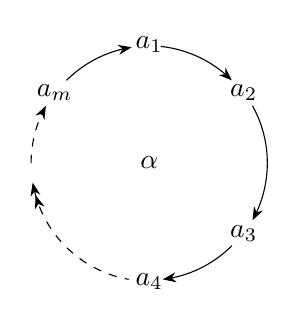
\begin{tikzpicture}[=>stealth]
%\draw(0,0)circle [radius = 1.5cm];
\draw(0,0)node[]{$\alpha$}
(0,1.5)node[]{$a_1$}
(0,-1.5)node[]{$a_4$}
(1.2,0.9)node[]{$a_2$}
(1.2,-0.9)node[]{$a_3$}
(-1.2,.9)node[]{$a_m$};
\draw(1.5,0)arc[start angle = 0, end angle = 29, radius = 1.5cm];
%\draw[-Stealth](1.5,0)arc[start angle = 360, end angle = -30, radius = 1.5cm];
\draw[Stealth-](1.05,1.05)arc[start angle = 45, end angle = 84, radius = 1.5cm];
%\draw[-Stealth](-0.15,1.45)arc[start angle = 90, end angle = 143, radius = 1.5cm];
\draw[-Stealth](1.5,0)arc[start angle = 0, end angle = -29 , radius = 1.5cm];
%\draw[-Stealth](-1.5,0)arc[start angle = 180, end angle = 209, radius = 1.5cm];
\draw[-Stealth](1.05,-1.05)arc[start angle = -45, end  angle = -83, radius = 1.5cm];
\draw[dashed,-Stealth](-1.5,0)arc[start angle = 180, end angle = 151, radius = 1.5cm];
\draw[-Stealth](-1.05,1.05)arc[start angle = 135, end angle = 99 , radius = 1.5cm];
\draw[dashed, {Stealth[sep = 0.25cm]Stealth[]}-](-1.5,0)arc[start angle = 180, end angle = 260, radius = 1.5cm]; %%%%%%%%%
\end{tikzpicture}
 &&&&&&&
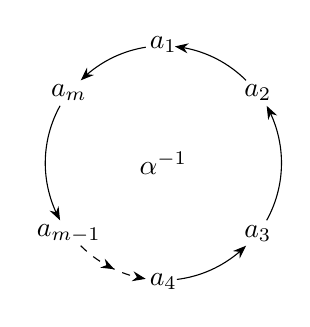
\begin{tikzpicture}[=>stealth]
%\draw(0,0)circle [radius = 1.5cm];
\draw(0,0)node[]{$\alpha^{-1}$}
(0,1.5)node[]{$a_1$}
(0,-1.5)node[]{$a_4$}
(1.2,0.9)node[]{$a_2$}
(1.2,-0.9)node[]{$a_3$}
(-1.2,.9)node[]{$a_m$}
(-1.2,-.9)node[]{$a_{m-1}$};
\draw[-Stealth](1.5,0)arc[start angle = 0, end angle = 29, radius = 1.5cm];
%\draw[-Stealth](1.5,0)arc[start angle = 360, end angle = -30, radius = 1.5cm];
\draw[-Stealth](1.05,1.05)arc[start angle = 45, end angle = 84, radius = 1.5cm];
%\draw[-Stealth](-0.15,1.45)arc[start angle = 90, end angle = 143, radius = 1.5cm];
\draw(1.5,0)arc[start angle = 0, end angle = -29 , radius = 1.5cm];
\draw[-Stealth](-1.5,0)arc[start angle = 180, end angle = 209, radius = 1.5cm];
\draw[Stealth-](1.05,-1.05)arc[start angle = -45, end  angle = -83, radius = 1.5cm];
\draw(-1.5,0)arc[start angle = 180, end angle = 151, radius = 1.5cm];
\draw[Stealth-](-1.05,1.05)arc[start angle = 135, end angle = 99 , radius = 1.5cm];
\draw[dashed, -{Stealth[sep = .25cm]Stealth[]}](-1.05,-1.05)arc[start angle = 225, end angle = 261, radius = 1.5cm]; %%%%%%%%%
\end{tikzpicture}\\\\
\end{tabular}
\end{table}
\end{defn}












\begin{exa}
$\, \alpha = (1\, 2\,3)\hspace{0.3cm} \alpha^{-1} = (3\, 2\, 1)$\\
\end{exa}

\textit{Check that} $\, \, \alpha\alpha^{-1} = (1\,2\, 3)(3\,2\,1) = (1)\,$ (An identity map)
$$\begin{pmatrix}
1 & 2 & 3 \\
2 & 3 & 1\\
\end{pmatrix}\begin{pmatrix}
3 & 2 & 1\\
2 & 1 & 3\\
\end{pmatrix} = \begin{pmatrix}
1 & 2 & 3\\
1 & 2 & 3\\
\end{pmatrix}$$\\\\





\begin{defn}
A cycle of length 2 is called a transposition.\\\\
\end{defn}






\begin{thm}
Every permutation can be written as a product of transposition.\\
\end{thm}

\begin{proof}
Consider the $r$ cycle (cycle of length $r$). If then $\beta$ is the identity.\\
e.g $\, \, \begin{pmatrix}
1 & 2 & 3\\
1 & 2 & 3\\
\end{pmatrix} = (2\,3)(3\,2) = 1$ an identity map.\\
So $\beta = (1\,2)(1\,2)$ since $\, (1\, 2)^{-1} = 12$.\\
If $r\geq 2$, then $\beta = (1\, 2\, 3\,\cdots\cdots\, r)$ which can be written a $\beta = (1\,r)(1\,(r-1))\cdots\cdots (1\,2)$.\\\\
\end{proof}




\begin{exa}
Factorise into transpositions
\end{exa}
\begin{enumerate}
\item[(a)] $(1\,2\,4\,5\,3) = (1\,3)(1\,5)(1\,4)(1\,2)$
\item[(b)] $(1\,3\,2)(1\,2\,3) = (1\,2)(1\,3)(1\,3)(1\,2)$\\
\end{enumerate}

\begin{note}
\begin{enumerate}
\item[•] These transpositions in the factorisation need not commute. This is true if they are not disjoint. E.g $(1\,3)(1\,2)\neq (1\,2)(1\,3)$
\item[•] The factors of the factorisation are not uniquely determined.\\\\
\end{enumerate}
\end{note}







\begin{defn}
A permutation $\alpha \in S_n$ is even if it can be factorised into a product of an even number of transposition, otherwise it is old.\\


The \textit{parity} of a permutation is whether it is even or old.\\\\
\end{defn}





\begin{defn}
Two permutations $\alpha\,,\, \beta\in S_n$ are said to have same cycle structure if their complete factorisations have the same number of $r-$cycles for each $r$.\\\\
\end{defn}


\begin{note}
These are $\, \dfrac{1}{r}[(n(n-1)(n-2)\, \cdots\cdots\, (n-r+1)]\,$ $r-$cycles in $S_n$. E.G. The number of permutation in $S_7$ of the form $(abc)(de)$ is $\, \dfrac{1}{3}[7\cdot 6\cdot 5]\cdot\dfrac{1}{2}[4\cdot 3] = 70\cdot 6 = 420$\\\\
\end{note}


\begin{remark}
If $\alpha\, ,\, \gamma\in S_n$, then $\alpha\, \gamma\,\alpha^{-1}$ has the same Cycle structure as $\gamma$.\\
\end{remark}


\begin{exe}
Find the number of permutations with cycle structure of the form $(ab)(cd)\,$ in $S_4$ $\hspace{0.5cm} 1\,\, 2\, \, 3\,\, 4$\\ $ \hspace{0.3cm} n = 4$
$$\dfrac{1}{2}\,\Big[\dfrac{1}{r}\, (a\, b) \cdot \dfrac{1}{r}\Big] = \dfrac{1}{2}\Big[\dfrac{1}{2}\,(4\cdot 3)\cdot \dfrac{1}{2}\, (2\cdot 1)\Big] = \dfrac{1}{2}\, 6 = S$$\\
\end{exe}


\begin{note}
A cycle of odd length is even whilst that of even length is odd.\\\\
\end{note}



\begin{defn}
Let $\alpha\in S_n$ such that its complete factorisation into disjoint cycles is $\, \alpha = \beta_1\beta_2\cdots\cdots\beta_t$, then;  Signum $\alpha$ defined as $Sgn = (-1)^{n-t}$
\begin{enumerate}
\item[(a)] If $\gamma$ is a $1-$cycle, then the $Sgn(\gamma)= 1$ since then $n = t$.\\ $\implies \, Sgn(\gamma) = (-1)^{n-t} = (-1)^0 = 1$.
\item[(b)] If $\zeta$ is a transposition, then it mean $t = \underbrace{(n-2)}_{fixed}+ \underbrace{1}_{transposition} = n-1$. So\\ $\, Sgn(\zeta) = (-1)^{n-(n-1)} = -1^1 = -1$\\\\
\end{enumerate}
\end{defn}








\begin{prop}
\begin{enumerate}
\item[(i)] If $\, \alpha\, , \, \zeta\in S_n$, where $\zeta$ is a transposition, then $\,Sgn\, \zeta(\alpha) = -\, Sgn(\alpha)$.
\item[(ii)] For all $\, \alpha\, , \, \beta \in S_n\, , \, Sgn(\alpha\beta) = Sgn(\alpha)\,Sgn(\beta)$\\
\end{enumerate}

In general; $\, Sgn(\alpha_1\alpha_2\cdots\cdots \alpha_k) = Sgn(\alpha_1)\, Sgn(\alpha_2)\cdots\cdots Sgn(\alpha_k)$\\\\
\end{prop}

\begin{proof}
\subhead{(i)}
Multiplying a permutation by a transposition changes the number of inversions by
an odd amount, so it reverses parity. Hence
$\operatorname{Sgn}(\alpha\zeta) = -\operatorname{Sgn}(\alpha)$.

\subhead{(ii)}
Write $\beta$ as a product of $k$ transpositions, so
$\operatorname{Sgn}(\beta) = (-1)^{k}$. Applying part (i) $k$ times to
$\alpha\beta$,
$$\operatorname{Sgn}(\alpha\beta) = (-1)^{k}\operatorname{Sgn}(\alpha)
= \operatorname{Sgn}(\alpha)\operatorname{Sgn}(\beta).$$
The general product formula follows by induction on the number of factors.
\end{proof}

\begin{note}
Part (ii) says the sign is a homomorphism from $S_n$ to $\{\pm1\}$. Its kernel is
the alternating group $A_n$, which is therefore normal in $S_n$ and of index two
for $n\geq2$ --- a fact obtained here without any computation, purely from the
homomorphism property.
\end{note}






\begin{thm}
Let $\alpha\in S_n$ be a permutation then if $Sgn(\alpha) = 1$, then $\alpha$ is even and if $Sgn(\alpha)  = -1$, then $\alpha$  is old.\\
\end{thm}

\begin{proof}
Recall that for every transposition $\zeta$, $\,\, Sgn(\zeta)  = -1$. Therefore suppose $\, \alpha = \zeta_1\, , \, \zeta_2\, \cdots\cdots\, \zeta_q$ is a function of $\alpha$ into transposition $\, Sgn(\alpha) = Sgn(\zeta_1)\,Sgn(\zeta_2)\,\cdots\cdots\, Sgn(\zeta_q) = (-1)^q$. Therefore\\
If $\, (-1)^q = 1$, then $q$ is even $\implies \alpha$ is even\\
If $\, (-1)q = -1$, then $q$ is odd $\implies \alpha$ is odd.\\\\
\end{proof}








\begin{exa}
Determine the parity of the following
\end{exa}
\begin{enumerate}
\item $\alpha = \begin{pmatrix}
1 & 2 & 3 & 4 & 5 & 6\\
2 & 6 & 3 & 1 & 5 & 4\\
\end{pmatrix}\hspace{1.5cm}
\beta = \begin{pmatrix}
1 & 2 & 3 & 4 & 5 & 6\\
1 & 6 & 4 & 4 & 3 & 2\\
\end{pmatrix}\,\,$ in $S_6$.\\\\


\begin{solution}
$\alpha = (1\, 2\, 6\, 4)(3)(5)\,\,$ thus $t = 3\, $ disjoint cycles, so that\\
\end{solution}

 $\, Sgn(\alpha) = (-1)^{n-t} = (-1)^{6-3} = (-1)^3 = -1$ hence $\alpha$ is odd.\\

$\beta = (1)(2\,6)(3\,4\,5)$, that $t=3\implies \, Sgn(\beta) = (-1)^{6-3} = -1$\\\\



\item Suppose $\, \gamma = \begin{pmatrix}
1 & 2 & 3 & 4 & 5 & 6\\
1 & 2 & 3 & 4 & 5 & 6\\
\end{pmatrix}$
$$\implies\, \gamma = (1)(2)(3)(4)(5)(6)\, \implies Sgn(\gamma) = (-1)^{6-6} = 1$$
Consider the subset of even permutations of $S_n$. Now, such (even)(even) $= $ even. Thus, this subset is closed under composition.\\\\
\end{enumerate}









\begin{defn}
The set of even permutations in $S_n$ is called the \textit{alternating group} denoted as $A_n$.\\\\
\end{defn}




\begin{exe}
Show/prove that $A_n$ satisfies the group axioms.\\


\begin{proof}
(\textit{By nemwine!!})\\
Let $\, \alpha\, , \, \beta $ and $\delta \in A_n$ (be even permutations) then;
\end{proof}
\begin{enumerate}
\item[(i)] $(\alpha\cdot\beta)\cdot \delta = \alpha\cdot(\beta\cdot\delta)\,$ since the product of even permutation is even $= 1$.
\item[(ii)] $\exists\, e = (1)\in \, A_n \ni \, \alpha(1) = (1)\alpha = \alpha\,$ which is even.
\item[(iii)] $\forall x\in A_n\, \exists \, \alpha^{-1}\in A_n\,\ni\, \alpha\alpha^{-1} = \alpha^{-1}\alpha = 1$ where $\alpha^{-1}$ is the inverse of $\alpha$.\\\\
\end{enumerate}
\end{exe}






\begin{exa}
$S_3 =\{(1)\, , \, (1\,2)\, , \, (1\,3)\, , \, (2\, 3)\,  ,\, (1\, 2\, 3)\, , \, (1\, 3\, 2)\}$\hspace{1cm}
$A_3 = \{(1)\, , \, (1\, 2\, 3)\, ,\, (1\,3\, 2)\}$\\
\end{exa}




\begin{exe}
List the elements of $S_4$ and hence all elements $A_4$.\\
\end{exe}

\begin{solution}
The elements of $S_4$ include;
% table of matrices

\begin{table}[H]
\centering
$\checkmark\, = \,$  Own Inverse\\
\vspace{0.5cm}
\begin{tabular}{lccl}
$\checkmark\,\,(1)\hspace{0.6cm} \begin{pmatrix}
1 & 2 & 3 & 4\\
1 & 2 & 3 & 4\\
\end{pmatrix} = (1)$ &&& $\checkmark\,\,(2)\hspace{0.6cm}\begin{pmatrix}
1 & 2 & 3 & 4\\
2 & 1 & 3 & 4\\
\end{pmatrix} = (1\, 2)(3)(4)$\\\\
$(3)\hspace{0.6cm}\begin{pmatrix}
1 & 2 & 3 & 4\\
3 & 1 & 2 & 4\\
\end{pmatrix} = (1\, 3 \, 2)(4)$ &&& $\checkmark\,\,(4)\hspace{0.6cm}\begin{pmatrix}
1 & 2 & 3 & 4\\
3 & 2 & 1 & 4\\
\end{pmatrix} = (1\, 3)(2)(4)$\\\\
$(5)\hspace{0.6cm}\begin{pmatrix}
1 & 2 & 3 & 4\\
2 & 3 & 1 & 4\\
\end{pmatrix} = (1\, 2\, 3)(4)$ &&& $\checkmark\,\, (6)\hspace{0.6cm}\begin{pmatrix}
1 & 2 & 3 & 4\\
1 & 3 & 2 & 4\\
\end{pmatrix} = (1)(2\, 3)(4)$\\\\
$(7)\hspace{0.6cm}\begin{pmatrix}
1 & 2 & 3 & 4\\
1 & 3 & 4 & 2\\
\end{pmatrix} = (1)(2\,3\,4)$ &&& $\checkmark\,\, (8)\hspace{0.6cm}\begin{pmatrix}
1 & 2 & 3 & 4\\
1 & 4 & 3 & 2\\
\end{pmatrix} = (1)(2\,4)(3)$\\\\
$(9)\hspace{0.6cm}\begin{pmatrix}
1 & 2 & 3 & 4\\
3 & 1 & 4 & 2\\
\end{pmatrix} = (1\, 3\,4\,2)$ &&& $\checkmark\,\, (10)\hspace{0.6cm}\begin{pmatrix}
1 & 2 & 3 & 4\\
3 & 4 & 1 & 2\\
\end{pmatrix} = (1\, 3)(2\,4)$\\\\
$(11)\hspace{0.6cm}\begin{pmatrix}
1 & 2 & 3 & 4\\
4 & 3 & 1 & 2\\
\end{pmatrix} = (1\, 4\, 2\,3)$ &&& $(12)\hspace{0.6cm}\begin{pmatrix}
1 & 2 & 3 & 4\\
4 & 1 & 3 & 2\\
\end{pmatrix} = (1\, 4\, 2)(3)$\\\\
$\checkmark\,\, (13)\hspace{0.6cm} \begin{pmatrix}
1 & 2 & 3 & 4\\
1 & 2 & 4 & 3\\
\end{pmatrix} = (1)(2)(4\,3)$ &&& $(14)\hspace{0.6cm}\begin{pmatrix}
1 & 2 & 3 & 4\\
1 & 4 & 2 & 3\\
\end{pmatrix} = (1) (2\, 4\, 3)$\\\\
$\checkmark\,\, (15)\hspace{0.6cm} \begin{pmatrix}
1 & 2 & 3 & 4\\
2 & 1 & 4 & 3\\
\end{pmatrix} = (1\,2)(3\,4)$ &&& $(16)\hspace{0.6cm}  \begin{pmatrix}
1 & 2 & 3 & 4\\
2 & 4 & 1 & 3\\
\end{pmatrix} = (1\, 2\, 4\, 3)$\\\\
$(17)\hspace{0.6cm}\begin{pmatrix}
1 & 2 & 3 & 4\\
2 & 3 & 4 & 1\\
\end{pmatrix} = (1\, 2\, 3\, 4)$ &&& $(18)\hspace{0.6cm}\begin{pmatrix}
1 & 2 & 3 & 4\\
4 & 1 & 2 & 3\\
\end{pmatrix} = (1\, 4\, 3\, 2)$\\\\
$(19)\hspace{0.6cm}\begin{pmatrix}
1 & 2 & 3 & 4\\
2 & 3 & 4 & 1\\
\end{pmatrix} = (1\, 2\, 3\, 4)$ &&& $(20)\hspace{0.6cm}\begin{pmatrix}
1 & 2 & 3  & 4\\
2 & 4 & 3 & 1\\
\end{pmatrix} = (1\, 2\, 4)(3)$\\\\
$(21)\hspace{0.6cm}\begin{pmatrix}
1 & 2 & 3 & 4\\
3 & 4 & 2 & 1\\
\end{pmatrix} = (1\, 3\, 2 \, 4)$ &&& $(22)\hspace{0.6cm}\begin{pmatrix}
1 & 2 & 3 & 4\\
3 & 2 & 4 & 1\\
\end{pmatrix} = (1\, 3\, 4)(2)$\\\\
$\checkmark\,\, (23)\hspace{0.6cm} \begin{pmatrix}
1 & 2 & 3 & 4\\
4 & 2 & 3 & 1\\
\end{pmatrix} = (1\, 4)(2)(3)$ &&& $\checkmark\,\, (24)\hspace{0.6cm}\begin{pmatrix}
1 & 2 & 3 & 4\\
4 & 3 & 2 & 1\\
\end{pmatrix} = (1\, 4)(2\, 3)$\\
\end{tabular}
\end{table}


Therefore, the elements of $A_4$.
$$A_4 = \{(1)\, ,\, (1\,2\,3)(4)\, ,\, (1\, 3\, 2)(4)\, , \, (1\, 3)(2\, 4)\, , \, (1\, 4\,2)(3)\,  , \, (1)(2\, 4\, 3)\, , \, (1\,2)(3\,4)\,,\, (1\, 4\, 3)(2)\, , \, (1\, 2\, 4)(3)$$ $$\,,\, (1\, 3\, 4)(2)\, ,\, (1\, 4)(2\,3)\}$$

$\therefore\,\, A_4$ has 12 elements.\\\\
\end{solution}














\begin{thm}
For $n>1$, the alternating group $A_n$ has $\dfrac{n!}{2}$ elements.\\
\end{thm}


\begin{proof}
For each old permutation $\alpha$ in $S_n$ the permutation $(1\,2)\alpha$ is even. Thus there are atleast as many even permutations as there are odd.\\
For $\beta$ an even permutation, $(1\,2)\beta$ is odd. So, there are atleast as many odd permutations as there are even ones.\\
Thus the number of even permutations is equal to the numbers of odd permutations. Now $\begin{vmatrix}
S_n\\
\end{vmatrix} = n! \implies \begin{vmatrix}
A_n\\
\end{vmatrix} = \dfrac{1}{2}\, n!$ where $\begin{vmatrix}
S_n\\
\end{vmatrix}  = $ length of $S_n$ (number of elements in $S_n$).\\\\\\
\end{proof}





\subsection{Subgroups}

\begin{defn}
A subset $H$ of a group $G$ is called a subgroup of $G$d if it is a group with respect to operation in $G$.\\\\
\end{defn}




\begin{note}
If $H$ is a subgroup of $G$ and $a\, , \, b\in H$, then $ab\in H$.\\\\
\end{note}






\begin{exa}
\begin{enumerate}
\item $(\mathbb{Z}\, , \, +)$ is a subgroup of $\, (\mathbb{R}\, , \, +)$.
\item With multiplication, $\{1\, , \, -1\}$ is a subgroup of \textit{non-zero}(identity is 1, but 0 has no multiplicative inverse, so we say non-zero) real numbers.
\item Every group is a subgroup of itself.
\item If $e$ is the identity of a group, then $\{e\}$ is a group of $G$.
\item For all $n,\, \, A_n$ is a subgroup of $S_n$.\\\\
\end{enumerate}
\end{exa}



\textbf{Notation:}\\
If $H$ is a subgroup of $G$, then denote it as $H\leq G$ or $H<G$.\\\\



\begin{lem}
Let $G$ be a group with operation $*$. Further, let $H$ be a subgroup of $G$.
\begin{enumerate}
\item[(a)] If $e'$ is the identity of $H$ and $e$ is the identity of $G$, then $e' = e$.
\item[(b)] If $a\in H$, then the inverse of $a$ in $H$ is the same as that of $a\in G$.\\\\\
\end{enumerate}
\end{lem}

\begin{proof}
Two cosets $aH$ and $bH$ are either equal or disjoint. Suppose they meet, say
$x\in aH\cap bH$, so $x = ah_1 = bh_2$ for some $h_1,h_2\in H$. Then
$a = bh_2h_1^{-1}$, and for any $h\in H$,
$$ah = b\left(h_2h_1^{-1}h\right) \in bH ,$$
so $aH\subseteq bH$. Symmetry gives the reverse inclusion, hence $aH = bH$.

Every element $g$ lies in the coset $gH$, since $e\in H$, so the cosets cover
$G$. Being pairwise disjoint and covering, they partition $G$.
\end{proof}

\begin{remark}
The map $h\mapsto ah$ is a bijection from $H$ to $aH$, so every coset has
exactly $\left|H\right|$ elements. Combining that with the partition gives
Lagrange's theorem immediately: $\left|G\right| = \left[G:H\right]\left|H\right|$.
This lemma is the whole content of that theorem, and the theorem is the first
result in the subject that could not have been guessed from the definitions.
\end{remark}








\begin{thm}[Cayley]
Every group $G$ is a subgroup of $S_n$ for some $n$.\\\\
\end{thm}





\begin{exa}
$\{-1\, ,\, 1\}$, multiplication\\
\end{exa}

$\{(1\,2)\, (1)\}\hspace{0.5cm}$ and $\hspace{0.5cm} S_3 = {(1)\, , \, (1\, 2)\, , \, (1\, 3)\,, \cdots\cdots}$\\
where $(1\,2)$ represents any element that is the multiplicative inverse of itself.\\

$\bullet \, \{-1\, , \, 1\}$ with multiplication is a subgroup of $S_3$.\\\\






\begin{defn}
Let $G$ be a group and let $H$ be a subset of $G$. Then $H$ is said to be a subgroup of $G$ if and only if
\begin{enumerate}
\item[(a)] $H$ is non-empty
\item[(b)] For all $\, a,\, b\in H\, , \,\,\, ab\in H$.
\item[(c)] If $a\in H,\,$ then $a^{-1}\in H$.\\\\
\end{enumerate}







\textbf{Proposition}[one-step subgroup test]\\
A subset $H$ of a group $G$ is a subgroup of $G$ if and only if $H\neq \emptyset$ and whenever $x,\, y\in H\, , \, \, xy^{-1}\in H$.\\
\end{defn}


\begin{proof}
If $H$ is a subgroup, then $H \neq \emptyset$, since $e\in H$. If $x,\, y\in H$, then $y^{-1}\in H$ by (c) in definition so that by (b) $xy^{-1}\in H$.\\
Conversely, suppose $H$ is a subset of $G$ such that $H\neq \emptyset$ and whenever $x,\, y\in H$ then $xy^{-1}\in H$. Now since $H\neq \emptyset$, it must contain an element say $h$. Take $x = y = h$, we see that $e = hh^{-1}\in H$. If $y\in H$, set $x= e$, we have $y^{-1} = ey^{-1}\in H$. Finally, we know that $(y^{-1})^{-1} = y$. Hence, $x\,, \, y\in H$, then $y^{-1}\in H = x(y^{-1})^{-1}\in H$. Therefore $H$ is  a subgroup.\\\\
\end{proof}







\textbf{Examples}
\begin{enumerate}
\item Let $G$ an Abelian group with identity $e$. Then $H = \{x\in G:\, x^2 = e\}$ is a subgroup of $G$. $\big[$Torston elts$\big]$.\\

\textbf{Check:}\\
Clearly, $H\neq \emptyset,\,\, e\in H$ since $e^2 = e$. For each $a, \, b\in H$ we have by definition, $a^2 = e\, ,$\\ $\, b^2 = e$. We need to show that $ab^{-1}\in H$ i.e  $(ab^{-1})^2 = e$. Now
\begin{align*}
(ab^{-1})^2 & = (ab^{-1})(ab^{-1}) \\
            & = aab^{-1}b^{-1}\hspace{0.5cm}(\text{Since}\hspace{0.2cm}G\hspace{0.2cm}\text{is Abelian})\\
            & = a^2 (b^{-1})^2 = a^2(b^2)^{-1}\\
            & = e(e)^{-1} = e^2 = e
\end{align*}
Therefore $\,  ab^{-1}\in H$, thus $\, H<G$.\\

\item Let $G = \mathbb{Z}_8$ (integers of modulo 8). Then $H = \mathbb{Z}_{8/2}$ is a subgroup of $G$.
$$\mathbb{Z}_8 = \{0,\, 1,\, 2,\, 3,\, 4,\, 5,\, 6,\, 7\}\hspace{0.4cm}\text{and}\hspace{0.4cm} \mathbb{Z}_{8/2} = \{0,\, 2,\, 4,\, 6\}$$
$Z_n \implies$ addition.\\


\textbf{Check}\\
$H\neq \emptyset$\\
Now, for $x\, y\in H$ we need to show that $\, xy^{-1}\in H$

\begin{table}[H]
\centering
\begin{tabular}{cc|c|c|c|c|c}
 &  & \multicolumn{4}{c}{$y$} & \\
 & $+$ & 0 & 6 & 4 & 2 & \\
\cline{2-6}
\multirow{4}{*}{$x$} & 0 & 0 & 6 & 4 & 2 & \\
& 2 & 2 & 0 & 6 & 4 & \\
& 4 & 4 & 2 & 0 & 4 & \\
& 6 & 6 & 4 & 2 & 0 & $=xy^{-1} \in H$\\
\cline{3-6}
\end{tabular}
\hspace{1.5cm}
\begin{tabular}{ccl}
\multicolumn{3}{c}{since base 8}\\
$0^{-1} = 0$  & since & $0 + 0 = 0$\\
$2^{-1} = 6$  &       & $2 + 6 = 8 = 0$\\
$4^{-1} = 4$  &       & $4 + 4 = 8 = 0$\\
$6^{-1} = 2$  &       & $ 6 + 2 = 8 = 0$\\\\
$xy^{-1} = x-y$ & & \\
\end{tabular}
\end{table}






\item Show that the set $H = \{(1)\, , \, (1\, 2\, 3)\}$ is not a subgroup of $S_3$.\\

\textbf{Check}\\
Let $x  = y  = (1\, 2\, 3)$\\

$(1\, 2\, 3)(3\, 2\, 1)  = \begin{pmatrix}
1 & 2 & 3\\
2 & 3 & 1\\
\end{pmatrix}\begin{pmatrix}
1 & 2 & 3\\
3 & 1 & 2\\
\end{pmatrix}=\begin{pmatrix}
1 & 2 & 3\\
1 & 2 & 3\\
\end{pmatrix}$\\

Let $x = (1)$ and $y = (1\, 2\, 3)\,\,\, y^{-1} = (3\, 2\, 1)\implies xy^{-1} = (1)(3\, 2\, 1)\not\in H$. Hence \\\\
\end{enumerate}








\begin{exe}
Show that $\, A_n < S_n \, \, \forall n$.\\

\begin{solution}
(\textit{By nemwine!!!)}\\
Let $S_n = \{a_1\, , \, a_2\, \cdots\cdots\, ,\, a_n\}$. Then $A_n = \{a_i:\, i = 1, \, 2, \, \cdots\cdots\}$ where $a_i$ is even and $a_i\in S_n$. Now, since $\begin{vmatrix}
S_n\\
\end{vmatrix} = n!$ we have that $\begin{vmatrix}
A_n\\
\end{vmatrix} = \dfrac{n!}{2}$, since the $\begin{vmatrix}
A_n\\
\end{vmatrix}$ divides $S_n$ into two sets of odd and even permutations. This implies if $\begin{vmatrix}
S_n\\
\end{vmatrix} = n!$ and $\begin{vmatrix}
A_n\\
\end{vmatrix} = k!$ then $k!  = \dfrac{n!}{2}\, \implies k! < n! \implies \begin{vmatrix}
A_n\\
\end{vmatrix} < \begin{vmatrix}
S_n\\
\end{vmatrix} \implies A_n < S_n\,\,\forall n\in N$.\\\\
\end{solution}
\end{exe}







\begin{thm}
Let $G$ be a group and $H$ and $K$ be subgroups of $G$. Then $H\cap K$ is a subgroup of $G$.\\
\end{thm}


\begin{proof}
$H\cap K\neq \emptyset$ since $e\in H$ and $e\in K\implies e\in H\cap K$. Now, let $h\in H\cap K$, then $h\in H$ and $h\in  K$. But $H$ is a subgroup, then $h^{-1}\in H$ and $h^{-1}\in K$. Thus, $h^{-1}\in H\cap K$. Finally, let $h,\,h'\in H\cap K$, then $h\in H$ and $h'\in H$. Now $H$ is a subgroup so $hh'\in H$ similarly $h\in K$ and $h'\in K$, $K$ is a subgroup, $hh'\in K$. Thus $hh'\in H\cap K$. Thus $H\cap K$ is a subgroup.\\\\
\end{proof}





\begin{note}
Given subgroup $H\, , \, K$ in $G$. Then union $H\cup K$ is \textit{not always} a subgroup of $G$.\\\\
\end{note}





\begin{exa}
in $\mathbb{Z}_6$\\
\end{exa}

$\mathbb{Z}_{6/2}\cup Z_{6/3}\, $ is not a subgroup of $\mathbb{Z}_6$
$$\mathbb{Z}_6 = \{0,\, 1,\, 2,\, 3,\, 4, \, 5\}\hspace{0.5cm} \mathbb{Z}_{6/2}= \{0,\, 2,\, 4\}\hspace{0.5cm} \mathbb{Z}_{6/3} = \{0,\, 3\}$$
$$\implies \, \mathbb{Z}_{6/2}\cup \mathbb{Z}_{6/3} \, \cong \, \mathbb{Z}_3\cup \mathbb{Z}_2 = \{0,\, 2, \, 3,\, 4\}$$
\begin{table}[H]
\centering
\begin{tabular}{c|c|c|c|c|}
$+$ & $0^{-1} = 0$ & $2^{-1} = 4$ & $3^{-1} = 3$ & $4^{-1} = 2$\\
\hline
0 & 0 & 4 & 3 & 2\\
2 & 2 & 0 & 5 & 4\\
3 & 3 & 1 & 0 & 5\\
4 & 4 & 2 & 1 & 0\\
\cline{2-5}
\end{tabular}
\end{table}

$5\not\in \{0,\, 2,\, 3,\,4\} = \mathbb{Z}_3\cup \mathbb{Z}_2.\hspace{0.3cm} \therefore\, \mathbb{Z}_3\cup \mathbb{Z}_2\,$ is not a subgroup.\\\\\\














\subsection{Cosets and Lagrange's Theorem}


\begin{defn}
Let $H$ be a subgroup of $G$. Define $aH = \{ah|\, h\in H\}$ and $Ha = \{ha|\, h\in H\}$ for $a\in G$. The set $aH$ is called the left coset of $H$ in $G$. $Ha$ is called the right coset of $H$ is $G$.\\\\
\end{defn}





\begin{note}
If the group operation is addition, then the left coset is $a + H$ and the right coset is $H + a$.\\\\
\end{note}


\begin{note}
Every element of the group is in $aH$. (every element of a group can be represented by $aH$).\\\\
\end{note}






\begin{exa}
Find all the left coset of $H = \{(1)\, , \, (1\,3)\}\,$ in $S_3$.\\
\end{exa}


\begin{solution}

$S_3 = \{(1)\, ,\, (1\,2)\, , \, (1\, 3)\,,\, (2\,3)\,,\, (1\,2\,3)\,,\,(1\,3\,2)\}$.\\

Let cosets are all $aH = \{ah:\, a\in S_n$ and $h\in H\}$
\begin{enumerate}
\item $a = (1) H = \{(1)\,,\,(1\,3)\} = H$

\item $a = (1\,2) \implies\, (1\,2)H = \{(1\,2)\, , \, (1\,3\,2)\}$

\item $(1\,3)H = \{(1\,3)\, ,\, (1)\} = H \hspace{1cm} a = (1\,3)$

\item $(2\, 3)H = \{(2\, 3)\, , \, (1\, 2\, 3)\} \hspace{1cm} a = (2\, 3)$

\item $(1\, 2\,3)H = \{(1\, 2\, 3)\, , \, (2\, 3)\}\hspace{1cm} a = (1\, 2\, 3)$

\item $(1\, 3\, 2)H = \{(1\, 3\, 2)\, ,\, (1\, 2)\}$
\end{enumerate}
$$ 1 = 3\hspace{1cm} 2 = 6\hspace{1cm} 4 = 5$$


Note that there are only three distinct cosets of $H$ in $G$,  since 
\begin{align*}
(1) H & = (1\, 3)H\\
(1\, 2)H & = (1\, 3\,2)H\\
(2\,3)H & = (1\, 2\, 3)H\\\\
\end{align*}
\end{solution}













\begin{exe}
Let $\, G = \mathbb{Z}_9\, , \, \, H = \mathbb{Z}_{9/3} \cong\, 3\mathbb{Z}_3$\\

Find all the left cosets of $H$ in $G$.\\
\end{exe}


\begin{solution}
$\mathbb{Z}_9 = \{0, \, 1,\, 2,\, 3,\, 4,\, 5,\, 6, \, 7,\, 8\}$

$\mathbb{Z}_{9/3} = \{0,\, 3,\, 6\}$\\

The left cosets are all $a + H$ such that $\, a\in \mathbb{Z}_9$





\begin{table}[H]
\centering
\begin{tabular}{rccl}
$(1)\hspace{0.5cm}0 + H =  \hspace{0.3cm}$\begin{tabular}{c|c|c|c|}
$+$ & 0 & 3 & 6\\
\hline
0 & 0 & 3 & 6\\
\end{tabular} &&& 
$(2)\hspace{0.5cm} 1  + H = \hspace{0.3cm} $\begin{tabular}{c|c|c|c|}
$+$ & 0 & 3 & 6\\
\hline
1 & 1 & 4 & 7\\
\end{tabular}\\
&&&\\\\
$(3)\hspace{0.5cm} 2 + H =  \hspace{0.3cm}$\begin{tabular}{c|c|c|c|}
$+$ & 0 & 3 & 6\\
\hline
2 & 2 & 5 & 8\\
\end{tabular} &&&
$(4)\hspace{0.5cm} 3 + H=  \hspace{0.3cm}$\begin{tabular}{c|c|c|c|}
$+$ & 0 & 3 & 6\\
\hline
3 & 3 & 6 & 0\\
\end{tabular}\\
&&&\\\\
$(5)\hspace{0.5cm} 4 + H = \hspace{0.3cm}$\begin{tabular}{c|c|c|c|}
$+$  & 0 & 3 & 6\\
\hline
4 & 4 & 7 & 1\\
\end{tabular} &&&
$(6)\hspace{0.5cm} 5 + H = \hspace{0.3cm}$\begin{tabular}{c|c|c|c|}
$+$ & 0 & 3 & 6\\
\hline
5 & 5 & 8 & 2\\
\end{tabular}\\
&&&\\\\
$(7)\hspace{0.5cm} 6 +  H = \hspace{0.3cm}$\begin{tabular}{c|c|c|c|}
$+$ & 0 & 3 & 6\\
\hline
6 & 6 & 0 & 3\\
\end{tabular} &&&
$(8) \hspace{0.5cm} 7 + H =\hspace{0.3cm}$ \begin{tabular}{c|c|c|c|}
$+$ & 0 & 3 & 6\\
\hline
7 & 7 & 1 & 4\\
\end{tabular}\\
&&&\\\\
$(9)\hspace{0.5cm} 8 + H = \hspace{0.3cm}$ \begin{tabular}{c|c|c|c|}
$+$ & 0 & 3 & 6\\
\hline
8 & 8 & 2 & 5\\
\end{tabular} &&&\\
\end{tabular}
\end{table}







\vspace{0.5cm}
\begin{table}[H]
\centering
$\therefore\hspace{1cm}$
\begin{tabular}{rccl}
$- (1)\hspace{0.6cm} 0 + H = \{0\, , \, 3\, , \, 6\}$ &&& $(2)\hspace{0.6cm} 1 + H = \{1\, , \, 4\, ,\, 7\}$\\\\
$\checkmark\, (3)\hspace{0.6cm} 2 + H = \{2\,, \, 5\, , \, 8\}$ &&& $(4)\hspace{0.6cm} 3 + H = \{3\, , \, 6\, , \, 0\}$\\\\
$(5)\hspace{0.6cm}  4  + H  = \{4\,  , \, 7\, , \, 1\}$ &&& $(6)\hspace{0.6cm} 5 + H = \{5\, , \, 8\, ,\, 2\}$\\\\
$-\,(7)\hspace{0.6cm} 6 + H =  \{6\, , \, 0\, , \, 8\}$ &&& $\cancel{(8)\hspace{0.6cm} 7  + H = \{7\, , \, 1\, , \, 4\}}$\\\\
$\checkmark \,(9)\hspace{0.6cm} 8 + H = \{8\, , \, 2\, , \, 5\}$ &&&\\
\end{tabular}
\end{table}
\vspace{0.8cm}
\end{solution}











\begin{defn}
Given a group $G$, the number of elements in $G$ denoted as $\begin{vmatrix}
G\\
\end{vmatrix}$ is called order of $G$.\\\\
\end{defn}






\begin{defn}
The order of an element $g\in G$ is the least positive integer $n$ such that $g^n = e$.\\

$\underbrace{\text{e.g the order}\hspace{0.3cm} g(1) = 1\, , \, (1\,2) = 2\,\, \, (1\, 2\, 3) = 3\hspace{0.3cm} \text{since}\hspace{0.3cm}(1)^1 = e\,\, \, (1\,2)^2 = e\hspace{0.3cm}\text{and}\hspace{0.3cm}(1\, 2\, 3) = e}_{\textit{By nemwine}}$\\\\
\end{defn}






\begin{note}
In case there is no such $n$, then we say $g$ is of infinite order. e.g integers $\mathbb{Z}$ with addition, $3\in \mathbb{Z}$ is of infinite order, but in $\mathbb{Z}_5, \, \, 3$ is of order 2. $\,$ i.e $3^2 = 3 + 5 = 6 = 0$.\\\\
\end{note}






\begin{defn}
In a group $G$, all elements $g\in G$ such that $g^2 = e$ are called torsion elements.\\\\


\textbf{E.g}(by nemwine)\\
$1\cdot (1\,2)\in S_n\hspace{0.5cm} n\geq 2$ is a torsion element since $(1\, 2)^2 = e$.\\

$2\cdot 3 \in \mathbb{Z}_6$ is a torsion element since $3^2 = 3 + 3 = 6 = 0$.\\\\\
\end{defn}















\begin{thm}
Let $H$ be a subgroup of $G$. Let $a\, , \, b\in G$, then 
\begin{enumerate}
\item[(i)] $a H = b H$ if and only if $b^{-1}a\in H$. In particular $aH = H$ if and only if $a\in H$.
\item[(ii)] If $a H\cap bH \neq \emptyset$, then $a H = b H$.
\item[(iii)] $\begin{vmatrix}
a H\\
\end{vmatrix} = \begin{vmatrix}
H\\
\end{vmatrix}\,$  ``where $\begin{vmatrix}
\cdot\\
\end{vmatrix} \implies$ number of elements"\\
\end{enumerate}






\pagebreak
\end{thm}
\begin{proof}
\begin{enumerate}
\item[(i)] Assume $a H = b H$, then  we show that $b^{-1}a\in H$ and assume $b^{-1}aH$ and then show that $aH = bH$.\\
Suppose $a H = b H$, then $ah_1 = bh_2$ for some $h_1\, , \, h_2\in H$. Then $a = bh_2h^{-1}_1 = bh_0$ where $h_0 = h_2h^{-1}_1\in H$. Since $a = bh_0$, then $b^{-1}a = h_0\in H$.\\
Conversely, suppose $b^{-1}a\in H$, we need to show that $a H = b H$. We have that $b^{-1}a\in H$ implies that $a = bh_0$ for some $h_0\in H$. If $x\in aH$, then $x = ah = bh_0\in bH\implies aH \subset bH\cdots\cdots(*)$. If $y\in H$, then $y = bh\implies y = ah^{-1}_0h\in aH$. (Since $a = bh_0$\\ $\implies b = ah_0^{-1}).\, \implies bH\subset aH\cdots\cdots (**)$.\\
By $(*)$ and $(**),\, \, aH = bH$.\\


\item[(ii)] If $x\in aH \cap bH$, then $x\in aH$ and $x\in bH. \implies x = ah_1$, and $x = bh_2\implies (ah_1 = bh_2)$ for some $h_1\, , \, h_2\in H$. We get $ah_1 = bh_2\implies b^{-1}a = h_2h_1^{-1}\in H$. So by (i) $\, aH = bH$.\\


\item[(iii)] To show that $\begin{vmatrix}
aH\\
\end{vmatrix} = \begin{vmatrix}
H\\
\end{vmatrix}$, we need a bijection $f: \, H \longrightarrow aH$. For each $h\in H$, define $f(h) \implies ah$. We need to show that $f$ as defined is one-one and onto. Suppose\\ $f(h_1) = f(h_2)$ in $aH$.
\begin{align*}
\implies\, & ah_1 = ah_2\\
\implies\, & a^{-1}ah_1 = a^{-1}ah_2\\
\implies\, & h_1 = h_2\hspace{0.5cm} \text{Hence one-one}
\end{align*}
Now for each element $y\in aH$, there must be some $h'\in H$ such that $y = ah'$. Thus $f(h') = ah' = y$. Hence we have that for onto. So that $f$ is a bijection. We have $\begin{vmatrix}
aH\\
\end{vmatrix} = \begin{vmatrix}
H\\
\end{vmatrix}$.\\\\
\end{enumerate}
\end{proof}




\begin{note}
The left cosets of $H$ in $G$ are either disjoint or equal. Hence the cosets $aH$ for $a\in G$ partition the group into a collection of non-empty pair wise disjoint subsets of $G$.\\\\\
\end{note}








\subsection{Lagrange's Theorem}
If $H$ is a subgroup of a finite group $G$, then $\begin{vmatrix}
H\\
\end{vmatrix}$ divides $\begin{vmatrix}
G\\
\end{vmatrix}$.\\

\begin{proof}
Suppose $\{a_1H\, , \, a_2H\, , \, \cdots\cdots\, \, a_kH\}$ is a family of distinct cosets of $H$ in $G$. Then $G = a_1H\cup a_2H \cup\, \cdots\cdots\, \cup a_kH$, since each $g\in G$ lies in some coset of $H = a_iH$ for some $i$. Moreover, we know that cosets $a_i H$ and $a_jH$ are disjoint. Therefore, $\begin{vmatrix}
G\\
\end{vmatrix} = \begin{vmatrix}
a_1 H\\
\end{vmatrix} + \begin{vmatrix}
a_2 H\\
\end{vmatrix} + \cdots\cdots + \begin{vmatrix}
a_k H\\
\end{vmatrix}$. But $\, \begin{vmatrix}
a_i H\\
\end{vmatrix} = \begin{vmatrix}
H\\
\end{vmatrix}$ for all $i$
$\implies \, \begin{vmatrix}
G\\
\end{vmatrix} = \begin{vmatrix}
H\\
\end{vmatrix} + \begin{vmatrix}
H\\
\end{vmatrix} + \cdots\cdots\cdots  = k \begin{vmatrix}
H\\
\end{vmatrix}.\,\,$
Thus $\begin{vmatrix}
H\\
\end{vmatrix}$ goes into $\begin{vmatrix}
G\\
\end{vmatrix}\, \, k$ times. Thus $\begin{vmatrix}
H\\
\end{vmatrix}$ divides $\begin{vmatrix}
G\\
\end{vmatrix}$\\\\
\end{proof}





\begin{defn}
The index of a group $H$ in $G$ is the number of cosets of $H$ in $G$. It is denoted as $\, \big[G\, :\, H\big]$.\\


\textbf{Note:} $\, \begin{vmatrix}
G\\
\end{vmatrix}  = \big[G\, :\, H\big]\begin{vmatrix}
H\\
\end{vmatrix}$\\\\
\end{defn}



\begin{exa}
\begin{enumerate}
\item Consider the example of $\, H = \{0\, , \ , 3\, , \, 6\}$ in $G = \mathbb{Z}_9$
\begin{align*}
G & = 0 + H\cup 1 + H\cup 2 + H\\
& = \{0, \, 3, \, 6\} + \{1, \, 4, \, 7\} \cup \{2, \, 5,\, 8\}\\\\
\begin{vmatrix}
G\\
\end{vmatrix} & = \begin{vmatrix}
\{0\, , \, 3\, , \, 6\}\\
\end{vmatrix} + \begin{vmatrix}
\{1\, , \, 4\, , \, 7\}\\
\end{vmatrix} + \begin{vmatrix}
\{2\, , \, 5\, , \, 5\}\\
\end{vmatrix}\\
& = 3\begin{vmatrix}
H\\
\end{vmatrix}
\end{align*}
Thus the index of $H$ in $G$ is 3.\\



\item Index of $\langle(12)\rangle$ is $S_3$.
\begin{align*}
\langle(12)\rangle & = \big\{(12)^n:\, 1\leq n\leq \begin{vmatrix}
(12)\\
\end{vmatrix}\big\} = \big\{(12)^n:\, 1\leq n\leq 2\big\} = \big\{(12)\, , \, (1)\big\}\\\\
\therefore\,\, \begin{vmatrix}
\langle(12)\rangle\\
\end{vmatrix} = 2\hspace{0.5cm},\hspace{0.5cm} \begin{vmatrix}
S_3\\
\end{vmatrix} = 6
\end{align*}
Therefore, $\big[S_3:\, \langle(12)\rangle\big] = \dfrac{6}{2} = 3$\\




\item Index $\langle 2\rangle$ in $\mathbb{Z}_{10}$.\\
$\langle 2\rangle = \{2\, , \, 4\, , \, 6\, , \, 8\, , \, 0\}\hspace{1cm}$ (here we use addition)\\
$\implies\, \, \langle 2\rangle = \big\{2^r:\, 1\leq r\leq 5\big\}\hspace{0.3cm}\implies 2 + 2 + 2 + 2+ 2 + 2 = 0$\\
$$\implies \, 2^5 = e$$
$$\begin{vmatrix}
\langle 2\rangle\\
\end{vmatrix} = 5\hspace{0.5cm},\hspace{0.5cm}\begin{vmatrix}
\mathbb{Z}_{10}\\
\end{vmatrix} = 10$$
$\therefore\,\, \big[\mathbb{Z}_{10}\, , \, \langle 2\rangle\big] = 2$\\\\
\end{enumerate}
\end{exa}








\textbf{Corollaries}
\begin{enumerate}
\item If $G$ is a finite group and $a\in G$, then the order of $a$ is a division of the order $G$.\\

\begin{proof}
Denote order of $a$ as $\begin{vmatrix}
a\\
\end{vmatrix}$. $\, \langle a\rangle$ is a subgroup of $G$. By Lagrange's theorem, $\, \begin{vmatrix}
\langle a \rangle\\
\end{vmatrix}$ divides $\begin{vmatrix}
G\\
\end{vmatrix}$. Thus, the order of $a$ divides the order of $G$.\\
\end{proof}


\item A group $G$ of prime order contains no subgroup other than $\{e\}$\\

\begin{proof}
This is a direct consequence of the Lagrange's theorem since a prime has no positive divisions other than 1 and itself.\\
\end{proof}


\item Every group of prime order is cyclic and is generated by any one of its non-identity elements.\\

\begin{proof}
If $a\in G\, ,\, \, a\neq e$. Then $\langle a\rangle \neq \{e\}$. Then by preceding corollary $\langle a\rangle = G$.\\\\
\end{proof}
\end{enumerate}





\begin{defn}
$G$ is said to be Cyclic when it is generated by a single element.\\\\
\end{defn}




\begin{note}
Lagrange's theorem does not say that if $k$ is a divisor of $\begin{vmatrix}
G\\
\end{vmatrix}$, then $G$ has a subgroup of order $k$. On the other hand, the following theorem is always true.\\\\
\end{note}





\begin{thm}
Let $G$ be a Cyclic group of (finite) order $n$. i.e $G = \langle a\rangle = \{e\, , \, a\, , \, a^2\, , \, \cdots\cdots\, a^{n-1}\}$.
\begin{enumerate}
\item[(i)] Every subgroup of $G$ is Cyclic.
\item[(ii)] If $1\leq k\leq n$, then $a^k$ generates a subgroup of order $\, \dfrac{n}{(k\, ,\, n)}\,$ where $(k\,,\, n)$ is the greatest common divisor of $k\,, \, n$.
\item[(iii)] For each positive divisor of $n,\, G$ has exactly one subgroup of order $d$.\\\\
\end{enumerate}
\end{thm}






\textbf{Examples}
\begin{enumerate}
\item $\mathbb{Z}_{12}\, $ has 12 elements.\\
$\implies\, \langle 1\rangle = \mathbb{Z}_{12}\,$ divisors of 12 are $1\, , \, 2\,,\, 3\, , \, 4\, ,\, 6\, , \, 12$\\

Possible subgroups will have orders.
$$\dfrac{12}{(1\, , \, 12)}\, , \, \, \dfrac{12}{(2\, , \, 12)}\, , \,\, \dfrac{12}{(3\, , \, 12)}\, ,\, \, \dfrac{12}{(4\, , \, 12)}\, , \,\, \dfrac{12}{(6\,\, 12)}\, , \, \, \dfrac{12}{(12\, ,\, 12)}$$
$$12\, , \, 6\, ,\, 4\, , \, 3\,,\, 2\, , \, 1$$
Hence $\mathbb{Z}_{12}$ has the following subgroups:
\begin{align*}
\mathbb{Z}_{12} & = \{0\, , \, 1\, , \, 2\, ,\, 3\,, \, 4\, , \, 5\, , \, 6\, , \, 7\, , \, 8\, , \, 9\, , \, 10\, , \, 11\}\cong \langle 1\rangle\\
\mathbb{Z}_{12/2} & = \{0\, , \, 2\, , \, 4\, , \, 6\, , \, 8\, , \, 10\}  = \langle 2\rangle\\
\mathbb{Z}_{12/3} & = \{0\, , \, 3\, , \, 6\, , \, 9\} \cong \langle 3\rangle\\
\mathbb{Z}_{12/4} & = \{0\, , \, 4\, , \, 8\} \cong \langle 4\rangle\\
\mathbb{Z}_{12/6} & = \{0\, ,\, 6\} \cong \langle 6\rangle\\
\mathbb{Z}_{12/12} & = \{0\} \cong \langle 0\rangle.
\end{align*}
One may construct the subgroup lattice.

% DIAGRAM 5



\begin{figure}[H]
\centering
\begin{tikzpicture}[=>stealth]
\draw(0,0)node[]{$\langle 0\rangle$}
(1,1)node[]{$\langle 6\rangle$}
(2,2)node[]{$\langle 3\rangle$};
\draw(0.3,0.3)--(0.7,0.7)
(1.3,1.3)--(1.7,1.7);
\draw(0,2)node[]{$\langle 2\rangle$}
(1,3)node[]{$\langle 1\rangle$}
(-1,1)node[]{$\langle 4\rangle$};
\draw(-0.7,1.3)--(-0.3,1.7)
(0.7,2.7)--(0.3,2.3);
\draw(-0.7,0.7)--(-0.3,0.3)
(0.3,1.7)--(0.7,1.3)
(1.3,2.7)--(1.7,2.3);
\end{tikzpicture}
\end{figure}



















\item Determine the subgroup lattice for $\mathbb{Z}_{p^2q}$, where $p\, q$ are prime.\\


\begin{solution}
Divisors for $\begin{vmatrix}
\mathbb{Z}_{p^2q}\\
\end{vmatrix}$ are $1\, , \, p\, , \, q\, , \, p^2\, , \, pq\,, \, p^2q$. Now each divisor $d$, there is a subgroup of order $d$.Namely 
$$\langle 1\rangle\, , \, \langle pq\rangle\,,\, \langle p^2\rangle\, , \, \langle q\rangle\, , \, \langle p\rangle \, , \, \langle 0\rangle$$
\end{solution}




% DIAGRAM D6
\begin{table}[H]
\centering
\begin{tabular}{ccccc}
generates (Subgroup order) &&& Subgroup Lattice &\\\\
$\langle 1\rangle = p^2q$ &&& 
\multirow{6}{*}{
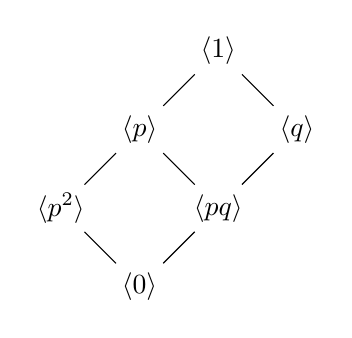
\begin{tikzpicture}[=>stealth]
\draw(0,0)node[]{$\langle 0\rangle$}
(1,1)node[]{$\langle pq\rangle$}
(2,2)node[]{$\langle q\rangle$};
\draw(0.3,0.3)--(0.7,0.7)
(1.3,1.3)--(1.7,1.7);
\draw(0,2)node[]{$\langle p\rangle$}
(1,3)node[]{$\langle 1\rangle$}
(-1,1)node[]{$\langle p^2\rangle$};
\draw(-0.7,1.3)--(-0.3,1.7)
(0.7,2.7)--(0.3,2.3);
\draw(-0.7,0.7)--(-0.3,0.3)
(0.3,1.7)--(0.7,1.3)
(1.3,2.7)--(1.7,2.3);
\end{tikzpicture}} &\\\\
$\langle p\rangle = pq$ &&& &\\\\
$\langle q\rangle = p^2$ &&& & \\\\
$\langle pq\rangle = p$ &&&&\\\\
$\langle p^2\rangle = q$ &&& & \\\\
$\langle 0\rangle = 1$ &&&&\\
\end{tabular}
\end{table}
\end{enumerate}






\vspace{1cm}
\subsection{Normal Subgroups}

\begin{defn}
A subgroup $K$ of a group $G$ is called a normal subgroup of $G$ (is normal in $G$) if for each element $k\in K$, and $g\in G$ we have $gkg^{-1}\in K$.\\\\
\end{defn}




\begin{note}
By this definition, then $K$ is normal in $G$ if for all $g\in G\hspace{0.3cm} gk = kg$ where $gk = kg \implies \, gk = k'g$ where $k\, , \, k'\in K$ or $k = k'$.\\
* $K$ ``commutes" as a set with elements of $G$.\\\\
\end{note}







\textbf{Examples}
\begin{enumerate}
\item The Cyclic group $H = \langle(12)\rangle$ of $S_3$ consisting of $(1)\,,\, (12)$ is not normal in $S_3$. Because.\\
Let for instance $\, g = (1\, 2\, 3)\, , \,\, g^{-1} = (3\, 2\, 1)$.\\
We have $\, g(12)g^{-1} = (1\, 2\, 3)(1\,2)(3\,2\,1) = (2\,3) \not\in H$. Hence $H$ is not normal in  $S_3$.\\


\item However, the Cyclic subgroup $\, \langle (1\, 2\, 3)\rangle\,$ of $S_3$ is a normal subgroup. (\textit{Check this is exercise})\\

$H = \langle(1\, 2\, 3)\rangle = \big\{(1\,2\,3)^n:\, 1\leq n\leq \begin{vmatrix}
(1\, 2\, 3)\\
\end{vmatrix}\big\} = \big\{(1\,2\,3)^n:\, 1\leq n\leq 3\big\} = \big\{(1\,2\,3)\, ,\, (1\, 3\, 2)\, , \, (1)\big\}$
\begin{enumerate}
    \item If $\, g = (1)$ then $g^{-1} = (1)\,\implies gkg^{-1} = k\in K$
    \item If $\, g = (1\, 2) \implies g^{-1} = (2\,1) \implies g(1\, 2\, 3)g^{-1} = (1\,2)(1\, 2\, 3)(2\,1) = (1\,3\, 2)\in K$
    \item If $\, g= (1\,3) \implies g^{-1} = (3\, 1) \implies g(1\, 2\, 3)g^{-1} = (1\,3)(1\,2\,3)(3\,1) = (1\,3\,2)\in H = K$
    \item If $\, g = (1\,2\,3) \, , \, g^{-1}(3\, 2\, 1) \implies g(1\,3\,2)g^{-1} = (1\, 2\, 3)(1\,3\,2) (3\,2\,1) = (1\,3\,2)\in K$
    \item If $\, g = (2\,3)\,,\, g^{-1} = (3\,2) \implies g(1\, 2\, 3)g^{-1} = (2\, 3)(1\,2\,3)(3\,2) = (1\,3\, 2)\in K$
    \item If $\, g = (1\, 3\,2) \, , \, g^{-1} = (2\, 3\, 1)\implies g(1)g^{-1}  = (1\, 3\, 2) (1)(2\,3\,1) = (1)\in K $\\
    
          $\therefore\, \, \forall\, g\in S_3$ and $k\in K\,\, gkg^{-1}\in K$\\
\end{enumerate}


\item Every subgroup $H$ of a Abelian group $G$ is normal in $G$.\\


\begin{proof}
If $G$ is an Abelian group, every subgroup $H$ of $G$ is normal in $G$ since, if $g\in G$, then $gH  = Hg\implies gHg^{-1} = H \implies gHg^{-1} \in H$. Let $h\in H$, then $ghg^{-1} \in H\,\, \forall\, h\in H$. Therefore, $H$ is normal in G.\\
\end{proof}



\item Let $H= SL(2\, ,\, \mathbb{R})\hspace{0.5cm} G = GL(2\, , \, \mathbb{R})$\\

$2 \implies \, 2\times 2\, $ matrices $\hspace{1cm} R \implies $ entries from $\mathbb{R}$.\\

Then $H$ is  a normal subgroup of $G$.
\begin{align*}
G = \Big\{\begin{pmatrix}
a & b\\
c & d\\
\end{pmatrix}\Big|\, a, \, b, \, c, \,  d\in \mathbb{R}\, \hspace{0.3cm} \text{and}\hspace{0.3cm}\begin{vmatrix}
a & b\\
c & d\\
\end{vmatrix} \neq 0\Big\}\\\\
H = \Big\{\begin{pmatrix}
a & b\\
c & d\\
\end{pmatrix}\Big|\, a,\, b,\, c,\, d\in \mathbb{R},\hspace{0.3cm} \text{and}\hspace{0.3cm} \begin{vmatrix}
a & b\\
c & d\\
\end{vmatrix} = 1\Big\}
\end{align*}

\begin{solution}
Clearly, $H\neq \emptyset$ because $\begin{pmatrix}
1 & 0\\
0 & 1\\
\end{pmatrix}\in H$. Now for any elements $A, \, B\in H$, we want to show that $AB^{-1}\in H$. 
\end{solution}
\begin{align*}
det\big(AB^{-1}\big)  & = \det(A)\cdot \det (B^{-1})
 = \det(A)\cdot \dfrac{1}{\det(B)}\\
& = 1\cdot 1/1 = 1\, \implies A,\, B^{-1}\in H
\end{align*}
i.e $H$ is a subgroup of $G$.\\
Now we check if $H\,\vartriangleleft\,G$ (if $H$ is normal in $G$). i.e, we want to show that, for $A\in H,\,\, B\in G,\,\, BAB^{-1}\in H$. Now 
\begin{align*}
\det\big(BAB^{-1}\big) & = \det B\cdot \det A\cdot \dfrac{1}{\det B}
 = \det (A) = 1
\end{align*}
Hence $\, BAB^{-1}\, $ and $\, H\lhd G$.\\\\
\end{enumerate}






\textbf{Exercise $*$}\\
Show that \begin{enumerate}
         \item $SL (n\, ,\, \mathbb{R}) \lhd GL(n\, ,\, \mathbb{R})$
         \item $SL (n\, , \, \mathbb{C})\lhd GL(n\,,\, \mathbb{C})$
         \item $SL (2n\, , \, \mathbb{R})\lhd GL(2n\, , \, \mathbb{R})$\\
\end{enumerate}

 
 
$4.$ For any $n, \, A_n \lhd S_n$.\\

\begin{proof}
Indeed $A_n < S_n$, we just need to show that it is normal in $S_n$.\\
Let $\alpha \in A_n \, ,\, \beta \in S_n$. We want to show that $\beta\alpha \beta^{-1}\in A_n$.\\
Now $Sgn\big(\beta\alpha\beta^{-1}\big) = Sgn(\beta)\, Sgn(\alpha)\, Sgn(\beta^{-1}) = Sgn(\beta)\, Sgn(\beta^{-1}) = 1$ (since if $\beta$ is even also $\beta^{-1}$  and if $\beta$ is odd so is $\beta^{-1}$). Thus $\beta\alpha\beta^{-1}$ is even $\,\implies \beta\alpha\beta^{-1}\in A_n$. Therefore $A_n\lhd S_n$.\\\\ 
\end{proof}





\begin{defn}
A group $G\neq \{e\}$ is called a \textit{simple group} if $G$ has no normal subgroups except $\{e\}$ and $G$.\\\\



$\bullet$ We now introduce some special subgroup which are normal in any group.\\\\
\end{defn}



\begin{defn}
Let $G$ be a group. Then center of $G$ denoted as $Z(G)$ is defined as $Z(G) = \{z\in G:\, zg = gz\, , \, $ for all $g\in G\}$.\\\\
\end{defn}




\begin{exe}
Show that the centre of a group $G$ is a normal subgroup of $G$.\\
\end{exe}

\begin{proof}
Let $\, z\in Z(G)$ and $g\in G$ then $zg = gz$ since $Z(G)$ is the centre of $G$. This implies that $z = gzg^{-1}\in Z(G)\,\, \forall g\in G$. Therefore\, $Z(G)$ is normal subgroup of $G$.\\\\
\end{proof}



\begin{note}
A group $G$ is Abelian if and only if $Z(G) = G$. On the other hand a group is said to \textit{centerless} if $Z(G) = \{e\}$.\\\\
\end{note}




\begin{exa}
\begin{enumerate}
\item $G = \Bigg\{\begin{pmatrix}
1 & a & c\\
0 & 1 & b\\
0 & 0 & 1\\
\end{pmatrix}:\, a,\, b,\, c\in \mathbb{R}\Bigg\}$  ``The Heisenberg Group".\\

Then $Z(G) = \Bigg\{\begin{pmatrix}
1 & 0 & d\\
0 & 1 & 0\\
0 & 0 & 1\\
\end{pmatrix}:\, d\in \mathbb{R}\Bigg\}$\\

To show this let $A =  G = \begin{pmatrix}
1 & a & c\\
0 & 1 & b\\
0 & 0 & 1\\
\end{pmatrix}\, $ and $\, B = \begin{pmatrix}
1 & 0 & d\\
0 & 1 & 0\\
0 & 0 & 1\\
\end{pmatrix}\,$ and show that $\, AB = BA$.\\


\item Let $G$ be non-Abelian and simple (i.e $G$ is not commutative and has no normal subgroup except $\{e\}$ and $G$). Then $Z(G) = \{e\}$.\\

\begin{proof}
\textit{by nemwine!!!}\\
Let $G$ be non-Abelian and simple. Then $G$ has only two normal subgroups $G$ and $\{e\}$ since $G$ is simple. Suppose $a,\, b\in G$ then $ab\neq ba$ since $G$ is non-Abelian. However, since $G$ is simple then $\, \forall g\in G\, \exists\, e\in G$ such that $ge = eg = ge\in G$. This implies that the only element of $G$  that commutes with all other elements is the identity $(e)$. Thus $\forall g\in G:\, g\neq e\in G\, ,\, g\not\in Z(G)\implies Z(G) = \{e\}$. Thus the center of one element only $(e)$.\\
\end{proof}


\item Let $G = D_n - $ dihedral group on an $n-g$ on of order $2n$.\\
If $n$ is odd, $Z(G) = \{e\}$.\\
If $n$ is even , $Z(G) = \{e\, , \, r_{180}\}$.\\\\
\end{enumerate}
\end{exa}








\begin{defn}
Let $x\, y\in G$, where $G$ is a group. The elements $x^{-1}y^{-1}xy$ in $G$ is called the \textit{commutator}. The elements $x^{-1}y^{-1}xy$ is dented as $[x\, , \, y]$.\\\\
\end{defn}





\begin{defn}
The subgroup of $G$ generated by all commutators is called the \textit{commutator subgroup of $G$}. We denote this as $G'$. It is sometimes known as the \textit{derived subgroup} of $G$.\\ (i.e $G' = \big\{\langle x^{-1}y^{-1}xy\rangle\, x,\, y\in G\big\}$.\\\\
\end{defn}


\textbf{Exercise $**$}
\begin{enumerate}
\item Find $G',\,$ if $G = \mathbb{Z}^*_{12}\, - $ where $\mathbb{Z}^*_{n} = $ multiplicative group $\, \mathbb{Z}^*_{\rho} = \{x\in \mathbb{Z}_n:\, (x\, , \, n) = 1\}$.
\item Find $\, G',\, $ if $G = S_3$\\


e.g $\, \mathbb{Z}^*_{6} = \{1\, ,\, 5\}$\\

$\mathbb{Z}^*_{12} = \{1,\, 5,\, 7,\, 11\}$\\


$-\, U(n) = $ group of units $= \{x\in \mathbb{Z}_n:\, x^2 = 1\}$\\

e.g $U(8) = \{1,\, 3, \, 5\, 7\}$\\\\
\end{enumerate}






\begin{defn}
Let $A$ be a subset of $G$. The centraliser $C(A)$ of $A$ in $G$ is defined as\\ $C(A) = \{c\in G:\, ca = ac\,\,\forall a\in A\}$\\\\
\end{defn}



\begin{lem}
$C(A)$ is a normal subgroup of $G$.\\



\begin{proof}
(Exercise)\textit{(By nemwine!!!!)}\\
Let $A$ be a group of $G$ such that $\, \forall a\in A$ and $g\in G$, then $ca = ac$. This is a normal subgroup of $G$ since form $ca = ac$ we have that $a = cac^{-1}\in A\,\, \forall a\in A$. Thus $A\lhd G$.\\\\
\end{proof}
\end{lem}




\begin{lem}
If $A$ is an Abelian group, then $A$ is normal in $C(A)$.\\\\
\end{lem}

\begin{proof}
Let $A$ be abelian and let $C(A)$ be its centraliser, so every element of $C(A)$
commutes with every element of $A$. Take $a\in A$ and $c\in C(A)$. Then
$$cac^{-1} = acc^{-1} = a \in A ,$$
using that $c$ commutes with $a$. So $cAc^{-1}\subseteq A$ for every
$c\in C(A)$, which is precisely the statement that $A$ is normal in $C(A)$.
\end{proof}



\begin{defn}
The normaliser $N_G(A)$ of $A$ in $G$ is defined as; $$N_G(A) = \{n\in G:\, A_n = nA\} = \{n\in G:\, nA^{-1}n = A\}$$\\
\end{defn}




\textbf{Note;}\\
$N_G(A)$ is a subgroup of $G$. If $A$ is a subgroup, then $N_G(A)\lhd G$. In the case where $A$ is a subgroup of $G$, then $A\lhd G$ if and only if $N_G(A) = G$.\\\\














\begin{prop}
\begin{enumerate}
\item[(i)] If $H$ is a subgroup of index 2 in a group $G$, then $g^2\in H\,\,\, \forall g\in G$ or if $H$ is of index 2 then it contains all the squares.
\item[(ii)] If $H$ is a subgroup of index 2 in a group $G$, then $H\,\vartriangleleft\, G$.\\
\end{enumerate}
\end{prop}


\begin{proof}
\begin{enumerate}
\item[(i)] Since $H$ is of index 2, then $\begin{vmatrix}
G\\
\end{vmatrix} = 2\, \begin{vmatrix}
H\\
\end{vmatrix}$. Hence there are exactly two cosets, namely $H$ and $a H$ for $a\in H$ i.e $G = H\cup aH$. Let $g\in G\,\ni\, g\not\in H$, then $g = ah$ for some $h\in H$. If $g^2\not\in H$ then, $g^2 = ah'$ for some $h'\in H$. Then $g = g^{-1}g^2 = h^{-1}a^{-1}ah' = h^{-1}h'\in H$. This is a contradiction since it was assumed that $g\not\in H$. Hence $g^2\in H$.

\item[(ii)] To prove the second statement, it is sufficient to show that if $h\in H$, $\, \, ghg^{-1}\in H\,\,\, \forall g\in G$. $H$ is of index 2 in $G$ implies there are exactly 2 cosets namely $H$ and $aH$ for some $a\not\in H$. Let $g\in G$, then $g\in H$ or $g\in aH$. If $g\in H$, then clearly $ghg^{-1}\in H$ because $H$ is a subgroup.\\
If $ghg^{-1}\not\in H$, then, $ghg^{-1} = ah'a^{-1}\in aH$ so that; $ah'a^{-1} = ay$ for some $y\in H$. Canceling $a$, we have $h'a^{-1} = y$. This implies that $a = y^{-1}h'\in H$. This is a contradiction since $a\not\in H$. Therefore, $ghg^{-1}\in H$ so if $h\in H$ then every. Conjugate of $h$ also lies in $H$. Hence $H\vartriangleleft G$.\\
\end{enumerate}
\end{proof}







\begin{defn}
If $H$ is a subgroup of a group $G$, then the conjugate of it is a subgroup of $G$ of the form; $\, aHa^{-1} = \{aha^{-1}\, :\, h\in H\}\,$ where $a\in G$.\\\\
\end{defn}



\begin{defn}
If $H$ and $K$ are subgroups of a group $G$, we say that $H$ and $K$ are conjugate in $G$ if $\, \exists\,$ an element $g\in G$ such that $H = gKg^{-1}$.\\\\\\
\end{defn}




\textbf{SOLUTIONS TO THE ASSIGNMENT}
\begin{enumerate}
\item[(i)] Suppose $H$ and $K$ are subgroups of $G$ with $K\vartriangleleft G$. Then $HK = \{hk\, |\, h\in H\, ,\, k\in K\}$.
Clearly, $HK\neq \emptyset$ since $e\cdot e = e\in HK$ for some $e\in H$ and $e\in K$  since both $H$ and $K$ are subgroups. Now we must show that if $a$ and $b$ are in $HK$ then $ab^{-1}\in HK$. Let $a = h_1k_1$ and $b = h_2k_2$ for  $h_1\, , h_2\in H$ and $k_1\, , k_2\in K$. Then $$ab^{-1} = h_1k_1(h_2k_2)^{-1} = h_1k_1k_2^{-1}h_2^{-1} = h_1ek_1k_2^{-1}h_2^{-1} = h_1h_2^{-1}h_2k_1k_2h_2^{-1}$$ 
$\implies h_1h_2^{-1}\in H$ and $h_2k_1k_2^{-1}h_2^{-1}\in K$ since $K\vartriangleleft G$.\\ Hence $ab^{-1} = h_1k_1(h_2k_2)^{-1}\in HK$, so $HK$ is a subgroup of $G$.


\item[(ii)] Let $g\in G$ and $x\in HK$. Then $x = hk$ for some $h\in H$ and $k\in K$. Thus\\ $gxg^{-1} = g(hk)g^{-1} = \big(ghg^{-1}\big)\big(gkg^{-1}\big)\in HK$ (since $ghg^{-1} \in H$ and $gkg^{-1}\in K$). This proves that $HK$ is a normal subgroup of $G$.\\\\
\end{enumerate}








\textbf{Solutions to Exercise ``*"}
\begin{enumerate}
\item[(a)] Let $G = GL_{(n,\mathbb{R})}$ and $N = SL_{(n,\mathbb{R})}$. We need to show that $gxg^{-1}\in N\,\, \forall x\in N$ and $g\in G$. This translates into the case of $P$ invertible matrices. Any invertible matrix $P$ and $\det (A) = 1$, we have $PAP^{-1} = 1\, \,$ since $$\det \big(PAP^{-1}\big) = \det (P)\, \det (A)\, \dfrac{1}{\det (P)} = \det (A) = 1$$
Thus $\, \forall A\in N$ and $P$ an $n\times n$ invertible matrix in $G$, we obtain $PAP^{-1}\in N$. Hence $SL_{(n,\mathbb{R})}\vartriangleleft GL_{(n,\mathbb{R})}$.\\

\item[(b).]
\end{enumerate}


\vspace{4cm}







\pagebreak
\textbf{Exercise ``**"}
\begin{enumerate}
\item $\mathbb{Z}^*_{12} = \{x\in \mathbb{Z}\, :\, (x,12) = 1\}$\\
$\implies\, \mathbb{Z}^*_{12} = \{1\, , \, 5\, , \, 7\, , \, 11\}\,$ here, the identity is 1 implying ($*$ is multiplication)\\
$\implies\, \big(\mathbb{Z}^*_{12} = \big\{1\, , \, \frac{1}{5}\, , \, \frac{1}{7}\, , \, \frac{1}{11}\big\}$\\

Thus, $\, \forall x\in \mathbb{Z}^*_{12}\,$ we have $xx^{-1} = e\cdot = 1$. Hence $\, G' = \{1\}$ since\\ $\, G' = \{\langle x^{-1}y^{-1}xy\rangle = \langle 1\rangle = 1\}\,\, \forall x\, ,\,y \in \mathbb{Z}^*_{12}$\\


\item $G = S_3 = \{(1)\, , \, (12)\, , \, (13)\, , \, (23)\,, \, (123)\, , \, (132)\}$\\
We know that $(1)$ is an identity $\, \implies\, \forall x\in S_3\hspace{0.5cm} xe = ex = x$. To identify any other commutator element we try to pair the elements in $S_3$.\\ $\, (12)(13) = (132)\ne (123) = (13)(12)$. Hence $(12)$ nor $(13)$ is a commutator. However we have $\, (21)(31)(12)(13) = (123)\,$ is also a commutator.\\
$(23)(123) = (13)(2)\neq (12)(3) = (123)(23)$. Hence neither $(123)$ nor $(23)$ is a commutator. However, $(32)(321)(23)(123) = (132)$ is a commutator.\\
\end{enumerate}


\textit{Proof} that  $132$ is a commutator
$$(123)(132) = (1)(2)(3) = (1)(2)(3) = (132)(123)$$
$$(1) = (1)$$
Hence $\, {[x,y]} = \{(1)\, , \, (123)\, , \, (132)\}$\\

Now $\, G' = \big\{\langle (1)\, , \, (123)\,  , \, (132)\rangle \big\} = \big\{(1)\, ,\, (123)\, , \, (132)\big\}$















\pagebreak

\subsection{Practice Problems}

\begin{problem}
Let $G$ be a group in which $g^{2}=e$ for every $g\in G$. Prove that $G$ is
abelian.
\end{problem}
\begin{solution}
The hypothesis says every element is its own inverse: $g^{2}=e$ gives
$g^{-1}=g$. For any $a,b\in G$ the product $ab$ is also an element, so
$$ab = (ab)^{-1} = b^{-1}a^{-1} = ba ,$$
using the reversal rule for inverses and then the hypothesis on $a$ and $b$
separately. Hence $G$ is abelian.

Such a group is a vector space over the field of two elements, so its order must
be a power of $2$ --- which the argument above does not show, but which explains
why no group of order $6$ can have this property.
\end{solution}

\begin{problem}
Show that a subgroup of index $2$ is normal.
\end{problem}
\begin{solution}
Let $[G:H]=2$, so there are exactly two left cosets, $H$ and $G\setminus H$, and
likewise two right cosets, $H$ and $G\setminus H$. Take $g\in G$.

If $g\in H$ then $gH = H = Hg$. If $g\notin H$ then $gH$ is the coset other than
$H$, so $gH = G\setminus H$; and $Hg$ is likewise the right coset other than
$H$, so $Hg = G\setminus H$. In both cases $gH = Hg$, which is normality.

The argument uses nothing about $G$ but the count. It fails at index $3$: the
subgroup $\left\{e,(12)\right\}$ of $S_3$ has index $3$ and is not normal, since
$(13)(12)(13)^{-1} = (23)$.
\end{solution}

\begin{problem}
Let $\phi: G\rightarrow H$ be a group homomorphism. Prove that $\ker\phi$ is a
normal subgroup of $G$ and that $\phi$ is injective if and only if
$\ker\phi=\{e\}$.
\end{problem}
\begin{solution}
\subhead{Normality}
$\ker\phi$ is a subgroup: $\phi(e)=e$, and if $\phi(a)=\phi(b)=e$ then
$\phi(ab^{-1}) = \phi(a)\phi(b)^{-1} = e$. For normality take $k\in\ker\phi$ and
$g\in G$:
$$\phi\left(gkg^{-1}\right) = \phi(g)\phi(k)\phi(g)^{-1}
= \phi(g)\,e\,\phi(g)^{-1} = e ,$$
so $gkg^{-1}\in\ker\phi$.

\subhead{Injectivity}
If $\phi$ is injective then $\phi(k)=e=\phi(e)$ forces $k=e$. Conversely, if the
kernel is trivial and $\phi(a)=\phi(b)$, then
$\phi\left(ab^{-1}\right)=e$, so $ab^{-1}=e$ and $a=b$.

Checking one element instead of every pair is the practical value here, and it
is why kernels are the standard route to injectivity.
\end{solution}


\section{GROUP ACTIONS}


\begin{defn}
Let $X$ be a set and $G$ a group. Then $G$ acts on $X$ if for each of $g\in G$, there is a function; $\,\, \alpha_g :\, X\longrightarrow X\,$ such that 
\begin{enumerate}
\item[(i)] $\alpha_g \cdot \alpha_h = \alpha_{gh}\,$ for $g\,,\, h\in G$.
\item[(ii)] $\alpha_e = 1_X$\\\\
\end{enumerate}
\end{defn}



\begin{exa}
\begin{enumerate}
\item $S_3 = \{(1)\,, \, (12)\, , \, (13)\, ,\, (23)\, , \, (123)\, ,\, (132)\}$\\
$X = \{(1)\, , \, (123)\, , \, (132)\}$\\

\textit{Check:} If $\, \forall g\, , \, h\in S_3\,$ and $\, x\in X$
\begin{enumerate}
      \item[(i)] $g\big(h(x)\big) = \big(gh\big)(x).$  $\hspace{0.5cm} 12(23(13)) = (23) = (12)(23)(13)$
      \item[(ii)] $(1)(x) = x$\\
\end{enumerate}


\item \underline{Trivial Action}. Given a group $G$, there exists the trivial action of $G$ on $G$ as follows; $\, g(x) = x\,\, \forall g\in G\, , \,\, x\in G$.
\begin{enumerate}
     \item[(i)] Let $g\, , \, h\in G$, and $\, x\in G$. $\, \,\,\, g\big(h(x)\big) = g(x) = x  = g\, h(x)$
     \item[(ii)] $e(x) = x$\\
\end{enumerate}


\item \underline{Regular Action}: Every group act on itself by multiplication on the left. $G\times G\, \longmapsto G\,$ defined by; $\, \, (g\, , \,x) \longmapsto gx\,\, \forall g\in G\, , \, x\in G$.
\begin{enumerate}
    \item[(i)] Let $g\, , \, h\in G$ and $x\in G$. Then $g\big(h(x)\big) = g\big(hx\big) = \big(gh\big)(x)$
    \item[(ii)] $e(x) = e\cdot x = x$\\
\end{enumerate}


\item \underline{Conjugation on Elements}\\
Define $\ g:\, x\longrightarrow gxg^{-1}\,$ where $g\in G\, ,\, x\in X$. The map as defined is an action of $G$ on $X$.
\begin{enumerate}
      \item[(i)] Let $g\, ,\, h\in G$ and $x\in X$. Then 
      \begin{align*}
      g\big(h(x)\big) & = g\big(hxh^{-1}\big) = ghxh^{-1}g^{-1}\\
                      & = (gh)x(gh)^{-1}\\
                      & = \big(gh\big)(x)
      \end{align*}
      \item[(ii)] $e(x) = e x e^{-1} = x$\\
\end{enumerate}


\item \underline{Conjugation on Subgroups}\\
Define $g:\, H\longmapsto gHg^{-1}$, where $g\in G$ and $H\leq G$
\begin{enumerate}
        \item[(i)] Let $g_1\, , \, g_2 \in G$. Then 
        \begin{align*}
        g_1\big(g_2(H)\big) & = \big\{g_1\big(g_2(h)\big)\, \big|\, h\in H\big\} = \big\{g_1\big(g_2hg_2^{-1}\big)\, \big|\, h\in H\big\}\\
                            & = \big\{g_1g_2hg_2^{-1}g_1^{-1}\,\big|\, h\in H\big\}\\
                            & = \big\{\big(g_1g_2\big)h\big(g_1g_2\big)^{-1}\, \big|\, h\in H\big\}\\
                            & = \big(g_1g_2\big)H
        \end{align*}
        
        \item[(ii)] $eH = \big\{ehe^{-1}\, \big|\, h\in H\big\} = \big\{h\, \big|\, h\in H\big\} = H$\\\\
\end{enumerate}
\end{enumerate}
\end{exa}



\begin{exe}
Show that the symmetric group $S_n$ and its subgroups acts on the set $X = \{1\, , \, 2\, , \ , \cdots\cdots\, , \, n\}$ by permuting its elements.
\begin{enumerate}
\item[(i)] Let $\, \alpha\, ,\, \beta\in S_n$, where $\alpha\,,\, \in S_n$ and let $x\in X$. Then $\alpha\big(\beta (x)\big) = \alpha\big(\beta x\big) = \alpha \beta (x) = \big(\alpha\beta\big) x$.\\\\
\end{enumerate}
\end{exe}










\begin{defn}
If $G$ acts on a set $SX$ and $x\in X$ then,
\begin{enumerate}
\item[(i)] The \textit{orbit} of $x$ denoted by $O(x)$ or $Orb_G(x)$ is defined by $\, O(x) = \{gx|\, g\in G\}$.
\item[(ii)] The \textit{stabilizer} of $X$, denoted by $Gx$ or $Stab_G(x)$ is defined by $\, Gx = \{g\in G|\, gx = x\}$.\\\\
\end{enumerate}
\end{defn}



\begin{note}
The action of $G$ on $X$ is said to be \textit{transitive} if there is only one orbit i.e for any $x\, , y\in X\, , \exists\, g\in G\ni gx  = y$.\\\\
\end{note}



\begin{note}
The stabilizer of $X$ in $G$ are all those elements of $G$ that leave $x$ fixed.\\\\
\end{note}



\begin{thm}
The stabilizer of $X$ in $G$ is a subgroup of $G$.\\
\end{thm}


\begin{proof}
Clearly, $G_X \neq \emptyset$, because $e\in G_X$ since $ex = x$. Now let $g\, , h\in G_X$, we have\\ $gh(x) = g\big(h(x)\big) = g(x) = x \implies gh \in G_X^{-*}$. Next we show that $g^{-1}\in G_X$ if $g\in G_X$. $\, g^{-1}(x)  = g^{-1}\big(g(x)\big) = \big(g^{-1}g\big)(x) = ex = x\implies g^{-1}\in G_X$. Now $\, g^{-1}h(x) \in G_X$.\\\\
\end{proof}




\begin{exa}
The group $G= \{(1)\, , \, (12)\,, \, (34)\, ,\, (12)(34)\}$ acts on the set $X = \{1\, ,\, 2\, ,\, 3\, , \, 4\}$
\begin{align*}
O(1) & = \{1\,,\, 2\} \hspace{0.4cm}\implies \, O(1) = (2)\\
O(2) & = \{1\, , \,2\}\\
O(3) & = \{3\, , \, 4\}\\
O(4) & = \{3\, , \, 4\}
\end{align*}


\begin{align*}
\text{Stabilizers are}\hspace{2cm} G_1 & = \{(1)\, , \, (34)\}\\
G_2 & = \{(1)\, , \, (34)\}\\
G_3 & = \{(1)\, , \, (12)\}\\
G_4 & = \{(1)\, , \, (12)\}\\\\
\end{align*}
\end{exa}




\begin{thm}[Orbit Stabiliser Theorem]
Let $G$ be a finite group acting on a set $X$ and let $x\in X$, then $\begin{vmatrix}
O(x)\\
\end{vmatrix} = \big[G:\, G_X\big]\,$ i.e $\, \begin{vmatrix}
G\\
\end{vmatrix} = \begin{vmatrix}
O(x)\\
\end{vmatrix}\,\begin{vmatrix}
G_x\\
\end{vmatrix}$.\\
\end{thm}


\begin{proof}
Let $G\big/G_X$ denote the family of cosets of $G_X$ in $G$. We want to exhibit a bijection $\phi$ between $O(x)$ and $G\big/G_X$. Let $y\in O(x)$, then $y = g(x)$ for some $g\in G$. Define $\phi (y) = g G_X$. Clearly, $\phi$ is single valued, because if $y = h(x)$ for some $h\in G$, then $h^{-1}g(x) = x$ and $h^{-1} g\in G_X$, hence $h G_X = g G_X$. To see that $\phi$ is one-one. Suppose $\phi (y) = \phi (z)$, then $\exists\,$ elements $h\, , g\in G\ni y = g(x)$ and $z = hx$ and $g G_X = h G_X$. That is $h^{-1}g\in G_X$. It follows that $h^{-1} g x = x$ and so $y = g(x) = h(x)  = z$.\\
Finally, we show that $\phi$ is onto. If $g G_X\in G\big/G_X$, then let $y = g x \in O(x)$ and note that $\phi (y) = g G_X$. Thus we have the bijection $\, \phi : \, O(x) \longrightarrow G\big/G_X \, \implies\, \begin{vmatrix}
O(x)\\
\end{vmatrix} = \begin{vmatrix}
G\big/ G_X\\
\end{vmatrix}$. Thus the proof.\\\\\
\end{proof}





\subsection{Class Equation}
Let $G$ be a finite group. Then the class equation of $G$ is , $$\begin{vmatrix}
G\\
\end{vmatrix} = \begin{vmatrix}
Z(G)\\
\end{vmatrix} + \sum_i\Big[G:\, C_G(x_i)\Big]$$ where $x_i$ is selected from each conjugacy class having \textit{more than one element}.

% DIAGRAM DM

\begin{figure}[H]
\centering
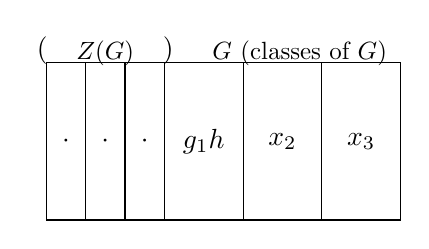
\begin{tikzpicture}
\draw(-1.5,-1)--(-1.5,1)
(-1,-1)--(-1,1)
(-0.5,-1)--(-0.5,1)
(0,-1)--(0,1)
(1,-1)--(1,1)
(2,-1)--(2,1)
(3,-1)--(3,1)
(-1.5,-1)--(3,-1)
(-1.5,1)--(3,1);
\draw(-1.25,0)node[]{$\cdot$}
(-0.75,0)node[]{$\cdot$}
(-0.25,0)node[]{$\cdot$}
(0.5,0)node[]{$g_1h$}
(1.5,0)node[]{$x_2$}
(2.5,0)node[]{$x_3$}
(0.5,1.12)node[right, scale=0.9]{$G$ (classes of $G$)}
(0.05,0.85)node[above]{$)$}
(-1.55,0.85)node[above]{$($}
(-0.75,0.85)node[above, scale = 0.9]{$Z(G)$};
\end{tikzpicture}
\end{figure}












\begin{enumerate}
\item[•] The elements in $Z(G)$ are conjugates of themselves, thus they form their own individual classes of $G$.
\item[•] Other elements in $G$ that are not self conjugates are paired with their conjugates in one class. i.e $(g\cdot h)$ above.\\\\
\end{enumerate}




\begin{defn}
Let $p$ be a prime number, then a $p-$group of order $p^n\, , \, \, n\geq 1$.\\\\
\end{defn}




\begin{thm}
It $p$ is a prime and $G$ is a $p-$group, then $Z(G)\neq \{e\}$.\\
\end{thm}

\begin{proof}
Consider the equation $\begin{vmatrix}
G\\
\end{vmatrix} = \begin{vmatrix}
Z(G)\\
\end{vmatrix} + \sum\limits_i\big[G:\, C_G(x_i)\big]$, each $C_G(x_i)$ is a proper subset of $G$ for each $x_i\not\in Z(G)$. Now, since $G$ is a $p-$group, $\big[G:\, C_G(x_i)\big]$ is a divisor of $p^n = \begin{vmatrix}
G\\
\end{vmatrix}$. Hence, it is itself a power of $p$. Thus $p$ divides both of the terms in the class equation other than $\begin{vmatrix}
Z(G)\\
\end{vmatrix}$, and so, $p\begin{vmatrix}
Z(G)\\
\end{vmatrix}$ as well. Therefore, $Z(G)\neq \{e\}$.\\\\
\end{proof}

 
 
 
 


\subsection{Quotient Groups} 

\begin{defn}
Let $(G\, , \, *)$ and $(H\, , \,\cdot)$ be groups (where $*\, ,\, \cdot\,$ are the respective operations in $G$ and $H$). Then the function $f:\, G\longrightarrow H$ is a \textit{homomorphism} if; $\, f(a*b) = f(a)\cdot f(b)\,\,\,\, \forall a\, , \, b\in G$.


% DIAGRAM D7
\begin{figure}[H]
\centering
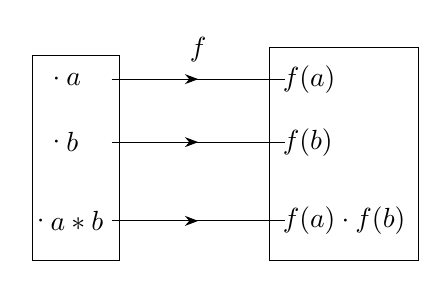
\begin{tikzpicture}[>=Stealth]
\draw(-0.9,-1.5)--(-0.9,1.1)--(-2,1.1)--(-2,-1.5)--cycle;
\draw(1,-1.5)--(1,1.2)--(2.9,1.2)--(2.9,-1.5)--cycle;
\draw(-1.7,0)node[]{$\cdot$}
(-1.7,0)node[right]{$b$}
(1.05,0)node[right]{$f(b)$}
(1.05,0.8)node[right]{$f(a)$}
(-1.7,0.8)node[]{$\cdot$}
(-1.7,0.8)node[right]{$a$}
(-1.9,-1)node[]{$\cdot$}
(-1.9,-1)node[right]{$a*b$}
(1.05,-1)node[right]{$f(a)\cdot f(b)$};
\draw[-{Stealth[]}](-1,0)--(0.1,0);
\draw(0,0)--(1.2,0);
\draw[-Stealth](-1,0.8)--(0.1,0.8);
\draw(0,0.8)--(1.2,0.8);
\draw[-Stealth](-1,-1)--(0.1,-1);
\draw(0,-1)--(1.2,-1);
\draw(0.1,0.9)node[above]{$f$};
\end{tikzpicture}
\end{figure}














\textbf{Note:} In the case where $f$ is a bijection, then we say it is an \textit{Isomorphism}\\\\
\end{defn}




\textbf{Example 1}
\begin{enumerate}
\item Let $G(\mathbb{R}\, ,\, +)\, , \,\, H = (\mathbb{R}\, ,\, X)$. Consider $f(x) = e^x$.  Show that $f$ is a homorphism.\\

\begin{solution}
Let $a\, , \, b\in (\mathbb{R}\, , \, +)$. Then $\, f(a + b) = e^{a+b} = e^a\cdot e^b = f(a)\cdot f(b)$.\\
\end{solution}


\item Let $A\, , \, B$ be groups, consider $\, \pi :\, A\times B \longrightarrow A$ divided by $\pi (a,b) = a$, where $a\in A\, , \, b\in B$. $\pi$ is a homorphism. Since for $(a,b)\, ,\, (a',b')\in A\times B$ for the direct product. We know that we can apply it pairwise as 
$$\pi\big[(a,b)(a',b')\big] = \pi(aa',bb') = aa' = \pi (a,b)\, \pi(a',b')$$
If we use addition, we have $\, \pi(a+a'\, , \, b+ b')$.\\\\
\end{enumerate}












\subsection{Some Fundamental Properties of Homomorphisms}
Let $Q:\, G\longrightarrow H$ be a homomorphism. Then the following are always true.
\begin{enumerate}
\item[•] $Q\big(e_G\big) = e_H$ (identity in $G$ should be sent to the identity in $H$).
\item[•] $Q\big(g^{-1}\big) = \big(Q(g)\big)^{-1}$, where $g^{-1}\in G\, , \, Q(g)\in H$.
\item[•] $Q\big(g^k\big) = \big(Q(g)\big)^k,$ where $g^k\in G\, ,\, Q(g)\in H$.
\item[•] $Q(g)$ is  a subgroup of $H$.
\item[•] If $Q$ one-to-one, then $G\approx Q(G)$. $(\approx$ Isomorphic to $Q(G))$. In this case, we say the subgroup $Q(G)$ is a \textit{homomorphic image} of the group $G$.\\\\
\end{enumerate}








\begin{defn}
Let $\, Q:\, G\longrightarrow H$ be a homomorphism, then the kernel of $Q$ denoted\\ $ker\, Q \, \cong\, \{g\in G:\, Q(g) = e_N\}$. Just like in vector space, all there elements sent to identity zero ``0" are Kernel(s).




% DIAGRAM D8



\begin{figure}[H]
\centering
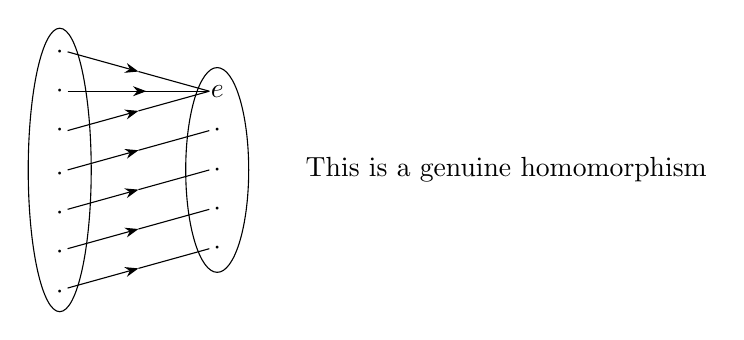
\begin{tikzpicture}[=>stealth]
\draw(-1,-0.05)node[]{$\cdot$}
(-1,0.5)node[]{$\cdot$}
(-1,1)node[]{$\cdot$}
(-1,1.5)node[]{$\cdot$}
(-1,-0.55)node[]{$\cdot$}
(-1,-1.05)node[]{$\cdot$}
(-1,-1.55)node[]{$\cdot$};
\draw(-1,0)ellipse[ x radius = 0.4cm , y radius = 1.8cm];
\draw(1,0)ellipse[x radius = 0.4cm , y radius = 1.3cm];
\draw(1,0)node[]{$\cdot$}
(1,0.5)node[]{$\cdot$}
(1,1)node[]{$e$}
(1,-0.5)node[]{$\cdot$}
(1,-1)node[]{$\cdot$};
\draw[-Stealth](-0.9,-1.5)--(0,-1.25);
\draw(0,-1.25)--(0.9,-1);
\draw[-Stealth](-0.9,-1)--(0,-0.75);
\draw(0,-0.75)--(0.9,-0.5);
\draw[-Stealth](-0.9,-0.5)--(0,-0.25);
\draw(0,-0.25)--(0.9,0);
\draw[-Stealth](-0.9,0)--(0,0.25);
\draw(0,0.25)--(0.9,0.5);
\draw[-Stealth](-0.9,0.5)--(0,0.75);
\draw(0,0.75)--(0.9,1);
\draw[-Stealth](-0.9,1)--(0.1,1);
\draw(-0.1,1)--(0.9,1);
\draw[-Stealth](-0.9,1.5)--(0,1.25);
\draw(0,1.25)--(0.9,1);
\draw(2,0)node[right]{\text{This is a genuine homomorphism}};
\end{tikzpicture}
\end{figure}
\end{defn}















\begin{thm}
Let $Q :\, G\longrightarrow H\,$ be a homomorphism, then $ker\, Q$ is a subgroup of $G$.\\
\end{thm}

\begin{proof}
$ker\, Q = \phi$ since $Q(e_G) = eH \implies e_G\in \, ker\, Q$. Let $g\, , \, h\in \, ker\, Q$, we check if $gh^{-1}\in \, ker\, Q$. 
\begin{align*}
Q\big(gh^{-1}\big) & = Q(g)\, Q\big(h^{-1}\big) = Q(g)\, \big(Q(h)\big)^{-1}\\
& = e_H\cdot\big(e_H\big)^{-1}\\
& = e_H
\end{align*}
$\therefore\, gh^{-1}\in\, ker\, Q$ and that it is a subgroup of $G$.\\\\
\end{proof}






\begin{exe}
Prove that $\,ker\, Q\,\underline{\Delta}\, G\, $ ($\underline{\Delta}$ means normal on).\\
\end{exe}

\begin{proof}
Let $G$ be a group and $ker \, Q$ be a subgroup of $G$ such that $\forall\, x\in G$ and $Q(x) = e_H$, then $x\in ker\, Q$. Let $g\in G$ and $x\in ker\, Q$, then 
\begin{align*}
Q(xg) & = Q(x)\, Q(g) = e_H\,Q(g) = Q(g) e_H\\
& = Q(g)\, Q(x)\\
& = Q(gx)
\end{align*}
So that $\, Q^{-1}Q(xg) = Q^{-1}Q(gx) \implies xg = gx \hspace{0.3cm} \forall g\in G$. Implying $gxg^{-1} = x\in ker\, Q\, \implies gxg^{-1}\in ker\, Q$. Thus $\, ker\, Q\, \underline{\Delta}\, G$.\\\\





\pagebreak
\end{proof}
\begin{exa}
Let $\, Q:\, \mathbb{Z}\longrightarrow \mathbb{Z}_n\,$ defined as follow. $\,Q(a  + b) = [a] + [b] = Q(a) + Q(b)$\\

e.g if we have $\mathbb{Z}_4$ split $[1][2][3][4]$
\begin{align*}
Z\longrightarrow \mathbb{Z}_4\hspace{2cm} 1 & = [1] = \{1,\, 5,\, 9,\, 13,\, 17,\, \cdots\cdots\}\hspace{0.5cm}\text{what it does is}\hspace{0.2cm}\mathbb{Z}_4\hspace{0.2cm}\text{split}\hspace{0.2cm}\mathbb{Z}\hspace{0.2cm}\text{into 4 graphs}\\
2 & = [2] = \{2, \, 6,\, 10,\, 14,\, \cdots\cdots\}\\
3 & = [3] = \{3,\, 7,\, 11,\, 15,\, \cdots\cdots\}\\
0 & = [0] = \{0,\, 4,\, 8,\, 12,\, 16,\, \cdots\cdots\}
\end{align*}
So, if we pick $(1 + 2) = 3$ which is in the next, so $\, ker\, Q = 0\in [0]$ $$5 + 6 = 1$$
Clearly, $Q$ is onto but not one-to-one.\\

What is $ker\, Q$, so we are looking for those elements in $Q(a + b)$ which will be sent to identity.\\
Note that for $\mathbb{Z}\longrightarrow \mathbb{Z}_n$ are $c  = 0 = [0]$.\\
What is $\, ker\, Q$?\\
The kernel of $Q$ consist of all multiples of $n$ since $Q(kn) = Q(k)\,Q(n) = Q(k)\cdot 0 = 0$ (since $Q(n) = 0$ which is the identity of $\mathbb{Z}_n$).\\


$\bullet$ For $\pi :\, A\times B \longrightarrow A$, find $\, ker\, \pi$. By definition
$$\pi (a,b)\longrightarrow a$$
$$\implies\, e(A,b) = e_A$$
We have $\, ker\, \pi = \big\{(e_A\, , \, b)\big|,\, e_A$ is identity for $A\, , b\in B\big\}$ because by definition $\, \pi(e_A\, , \, b) = e_A$.\\\\
\end{exa}







\begin{thm}
In the case where $Q:\, G\longrightarrow H\,$ is an isomorphism, then $\, ker\, Q = \{e_G\}$




% DIAGRAM 9
\begin{figure}[H]
\centering
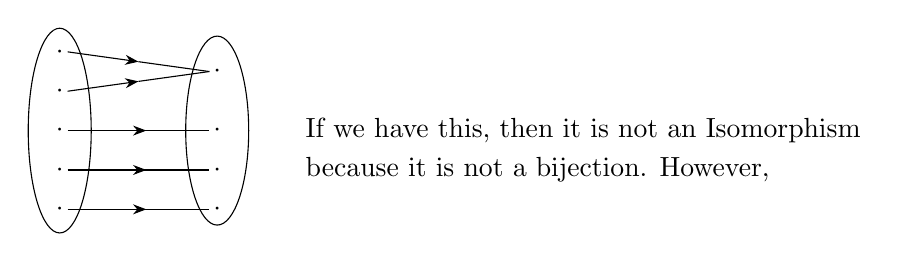
\begin{tikzpicture}[=>stealth]
\draw(-1,0)ellipse[x radius = 0.4cm, y radius = 1.3cm];
\draw(-1,0)node[]{$\cdot$}
(-1,0.5)node[]{$\cdot$}
(-1,1)node[]{$\cdot$}
(-1,-0.5)node[]{$\cdot$}
(-1,-1)node[]{$\cdot$};
\draw(1,0)ellipse[x radius = 0.4cm, y radius = 1.2cm];
\draw(1,0)node[]{$\cdot$}
(1,-0.5)node[]{$\cdot$}
(1,-1)node[]{$\cdot$}
(1,0.75)node[]{$\cdot$};
\draw[-Stealth](-0.9,0)--(0.1,0);
\draw[-Stealth](-0.9,-0.5)--(0.1,-0.5);
\draw[-Stealth](-0.9,-1)--(0.1,-1);
\draw(0,0)--(0.9,0)
(0,-0.5)--(0.9,-0.5)
(0,-1)--(0.9,-1);
\draw[-Stealth](-0.9,0.5)--(0,0.625);
\draw(0,0.625)--(0.9,0.75);
\draw[-Stealth](-0.9,1)--(0,0.875);
\draw(0,0.875)--(0.9,0.75);
\draw(2,0)node[right]{\text{If we have this, then it is not an Isomorphism}}
(2,-0.5)node[right]{\text{because it is not a bijection. However,}};
\end{tikzpicture}
\end{figure}











%DIAGRAM 10
\begin{figure}[H]
\centering
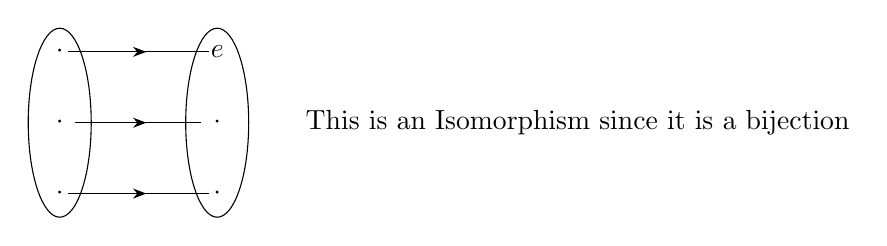
\begin{tikzpicture}[=>stealth]
\draw(-1,0)ellipse[x radius = 0.4cm, y radius = 1.2cm];
\draw(-1,0)node[]{$\cdot$}
(-1,-0.9)node[]{$\cdot$}
(-1,0.9)node[]{$\cdot$};
\draw(1,0)ellipse[x radius = 0.4cm, y radius = 1.2cm];
\draw(1,0)node[]{$\cdot$}
(1,0.9)node[]{$e$}
(1,-0.9)node[]{$\cdot$};
\draw[-Stealth](-0.8,0)--(0.1,0);
\draw(-0.1,0)--(0.8,0);
\draw[-Stealth](-0.9,-0.9)--(0.1,-0.9);
\draw(-0.1,-0.9)--(0.9,-0.9);
\draw[-Stealth](-0.9,0.9)--(0.1,0.9);
\draw(-0.1,0.9)--(0.9,0.9);
\draw(2,0)node[right]{\text{This is an Isomorphism since it is a bijection}};
\end{tikzpicture}
\end{figure}
\end{thm}

\begin{proof}
An isomorphism is injective. If $g\in\ker Q$ then $Q(g) = e_H = Q(e_G)$, and
injectivity forces $g = e_G$. Conversely $e_G$ always lies in the kernel. Hence
$\ker Q = \{e_G\}$.
\end{proof}

\begin{note}
The converse holds too and is the more useful direction: a homomorphism is
injective if and only if its kernel is trivial. Checking one element is easier
than checking every pair, which is why kernels are the standard tool for
proving injectivity.
\end{note}













\begin{note}
If you want to prove or see if it is an isomorphism start with a homomorphism then if it is a bijection (one-to-one) then it is an isomorphism.\\\\
\end{note}




\begin{exe}
Let $\, Q:\, G\longrightarrow H$. Suppose the $\, ker\, Q = \{e_G\}$, show that $Q$ is a bijection.\\\\
\end{exe}






\textbf{Proposition *}\\
Let $H$ and $K$ be subgroups of a group $G$
\begin{enumerate}
\item[(i)] If one of the subgroups $H$ or $K$ is a normal subgroup, then $HK$ is a subgroup of $G$.
\item[(ii)] If both $H$ and $K$ are normal, then $HK$ is normal in $G$.\\\\
\end{enumerate}




\begin{thm}[Properties of Subgroups Under Homomorphism]
Let $\, \phi :\, G\longrightarrow G'\,$ be a homomorphism and $H<G$, then
\begin{enumerate}
\item $\phi (H)$ is a subgroup of $G'$.
\item If $H$ is Cyclic, then $\phi(H)$ is Cyclic.
\item If $H$ is Abelian, then $\phi (H)$ is abelian.
\item If $H\, \Delta\, G$ then $\phi(H)\ , \Delta\, G'$.
\item If $\begin{vmatrix}
ker\, \phi\\
\end{vmatrix} = n$, then $\phi$ is an $n$ to 1 mapping from $G$ onto $\phi(G)$.
\item If $\begin{vmatrix}
H\\
\end{vmatrix} = n$, the $\begin{vmatrix}
\phi(H)\\
\end{vmatrix}$ divides $n$.
\item If $K <G'$, then $\phi^{-1}(K) < G$.
\item If $K\, \nabla\, G'$, then $\phi^{-1}(K)\, \nabla\, G$.
\item If $\phi$ is onto and $\, ker\, \phi = \{e\}$, then $\phi$ is an ismorphism.\\
\end{enumerate}





\begin{proof}
(exercise)\\\\
\end{proof}
\end{thm}



\begin{defn}
Let $X$ and $Y$ be non-empty subsets of a group $G$. Define a product $\, XY = \{xy|\, x\in X\, , \, y\in Y\}$.\\
We can easily show that $XY$ is associative. Suppose $X = Y = H$ is a subgroup of $G$. Then $HH = H$  is a subgroup of $G$. If $H$ and $K$ are subgroups of $G$, then $HK$ is not necessarily a subgroup of $G$.\\\\
\end{defn}





\begin{exa}
Let $G = S_3$ and $H = \langle (12) \rangle\, , \, K = \langle (13)\rangle$.\\
Then $\, HK = \{(1)\, , \, (12)\, , \, (13)\, , \, (132)\}$ is not a subgroup of $G = S_3$ since; 
\begin{enumerate}
\item[(i)] closure should be in there and the closure does not hold.
\item[(ii)] should be closed under inverse.
\begin{table}[H]
\centering
\begin{tabular}{cc|c|c|c}
 &  \multicolumn{3}{c}{$K$} & \\
 & & (1) & (13) & \\
\cline{2-4}
 \multirow{2}{*}{$H$} &(1) & (1) & (13) & \\
\cline{2-4}
  & (12) & (12) & (132)& $\longleftarrow\, \implies\, $ not closed under inverses\\
 \cline{2-4}
\end{tabular}
\end{table}




\item[(iii)] $\begin{vmatrix}
HK\\
\end{vmatrix}$ does not divide the order of $S_3$.
\end{enumerate}
However, under certain conditions a product of two subgroups may result into another subgroup.\\
Then \textbf{Proposition *} follows!!!\\\\
\end{exa}








\subsection{Fundamental Isomorphism}

\begin{thm}[$1^{\text{st}}$ Isomorphism Theorem]
Let $G$ and $H$ be groups, and let $Q:\, G\longrightarrow H$ be a homomorphism from $G$ to $H$, where $ker Q = K$, Then $\, G\big/K\, \cong \, H$.\\
\end{thm}


\begin{proof}
Define the map $\phi:\, G\big/K \, \longrightarrow H$ by $\phi (Ka) = Q(a)$ for each $Ka\in G\big/K$. We first show that $\phi$ is well defined.  If $Ka_1 = Ka_2$, then $Ka_1 = a_2$ for some $k\in K = ker Q$. So, $\, Q(Ka_1) = Q(a_2)$. But $$Q(Ka_1) = Q(K)\, Q(a_1) = e\, Q(a_1) = Q(a_1)$$
So that $\, Q(a_1) =  Q(a_2)$. Therefore, $Q(a)$ is determined solely by the cosets of $K$ to which $a$ belongs. So $\phi$ is well defined.\\
Next, we show that $\phi$ preserves the operation (it is a homomorphism). Let $Ka\, ,\, Kb\in G\big/K\, , $ then 
\begin{align*}
\phi\big((Ka)(Kb)\big) & = \phi\big(K(ab)\big)\\
& = Q(ab) = Q(a)\, Q(b)\\
& = \phi(Ka)\, Q(Kb)\hspace{0.5cm}\text{as required}
\end{align*}
Clearly, $\phi$ is  onto since $Q$ is. Finally, we show that $\phi$ is one-to-one. i.e , $ker\, \phi =$ identity $= \{Ke\}$. Indeed $ker\, \phi = \{Ke\}$ because, if $Ka \in ker\, \phi$, then $Q(a) = \phi (Ka) = e$ and therefore, $a\in ker\, Q = K$ i.e $Ka = K = Ke$. Thus $\phi$ is one-to-one.\\\\\\ 
\end{proof}











\begin{exa}
\begin{enumerate}
\item Every Cyclic group is a homomorphic image of $\mathbb{Z}$. i.e, Thus $G\cong \mathbb{Z}$ or $\, G\cong \mathbb{Z}\big/n\mathbb{Z}\,$ for some $n$.\\
Because, we may write $\, G = \langle g\rangle\,,$ if $\begin{vmatrix}
g\\
\end{vmatrix} = \infty\,, $ then $\, G\cong \mathbb{Z}$; if $\begin{vmatrix}
g\\
\end{vmatrix} = n$, then $\, G\cong \mathbb{Z}\big/n\mathbb{Z}$.

\item Consider the epimorphism  det$:\, G L_n(\mathbb{R})\longrightarrow \mathbb{R}^x$. Then $ker(det) = SL_n(\mathbb{R})$. Then $$GL_n(\mathbb{R})\big/SL_n(\mathbb{R}) \, \cong\, \mathbb{R}^x$$


Consider the group $G  = \Big\{\begin{pmatrix}
a & b\\
0& c\\
\end{pmatrix}\, , \, a\, , \, b\, , \, c\in \mathbb{R}\, , \, ac\neq 0\Big\}$ and $b\in \mathbb{R}^x$ ($b$ is non-negative).\\
Now, consider a map $\, f:\, G\longrightarrow \mathbb{R}^x$, defined by $f\Big(\begin{pmatrix}
a & b\\
0 & c\\
\end{pmatrix}\Big) = ac$.
\begin{enumerate}
\item[$-$] $f$ as defined is a hormomorphism since, for $\begin{pmatrix}
a & b\\
0 & c\\
\end{pmatrix}\, , \, \begin{pmatrix}
x & y\\
0 & z\\
\end{pmatrix}\in G$, 
$$f\begin{pmatrix}
\begin{pmatrix}
a & b\\
0 & c\\
\end{pmatrix} \begin{pmatrix}
x & y \\
0 & z\\
\end{pmatrix}
\end{pmatrix} = \begin{pmatrix}
ax & ay + bz\\
0 & cz\\
\end{pmatrix} = ax \, cz = ac\, xz = f\begin{pmatrix}
a & b \\
0 & c\\
\end{pmatrix}\cdot f\begin{pmatrix}
x & y\\
0 & z\\
\end{pmatrix}$$\\

\item[$-$] $f$ is onto (epimorphism).\\
for each $y\in \mathbb{R}^x\, \exists\, $ a matrix $\, \begin{pmatrix}
y & *\\
0 & 1\\
\end{pmatrix}\, \ni\, f\begin{pmatrix}
\begin{pmatrix}
y & *\\
0 & 1\\
\end{pmatrix}
\end{pmatrix} = y\cdot 1 = y$.\\\\


\item[$-$] $f$ is one-to-one i.e $\, kern(f)  = \Big\{\begin{pmatrix}
a & b\\
0 & a^{-1}\\
\end{pmatrix}\Big|\, a\, , \, b\in \mathbb{R}\Big\} = k$\\

Clearly, $\,\, G\big/K\,\, \cong \, \, \mathbb{R}^x$
\begin{align*}
GK  & = f\begin{pmatrix}
\begin{pmatrix}
a & b\\
0 & c\\
\end{pmatrix} \begin{pmatrix}
x & y\\
0 & x^{-1}\\
\end{pmatrix}
\end{pmatrix} = f\begin{pmatrix}
ax & ay + bx^{-1}\\
0 & cx^{-1}\\
\end{pmatrix}\\\\
& = acxx^{-1}
 = ac\in \mathbb{R}^x\\
\end{align*}
\end{enumerate}



\item Consider a symmetric group $S_n$ and the homomorphism $Sg_n :\, S_n \longrightarrow \{-1\,, \, 1\}$, has its kernel as $A_n$. Thus $\,S_n\big/A_n \, \cong \, \{-1\, , \, 1\}$\\\\
\end{enumerate}
\end{exa}







\begin{thm}[$2^{\text{nd}}$ Isomorphism Theorem]
Let $G$ be a group. Let $H\leq G$ and $K\trianglerighteq G$. Then $\, \, H K\big/ K\, \cong\, H\big/ H\cap K$.\\
\end{thm}


\begin{proof}
Routine verification shows that $HK$ is a group and that $K\trianglerighteq HK$ and that $H\cap K\trianglerighteq H$. Now, consider the map $H\longrightarrow HK\big/ K\hspace{0.3cm} h\longrightarrow hk$. This map has ker$H\cap K$ is surjuctive. So b the first isomorphism theorem, $\, \, H\big/H\cap K\, \, \cong \, \, HK\big/K$.\\\\






\textbf{Theorem ($3^{\text{rd}}$ Isomorphism Theorem)}``Absorption property of Cosets".\\
Let $G$ be a group. Let $K \trianglelefteq G$, and let $N\leq K$. Then $\, K\big/N\trianglelefteq G\big/N\,$ and $\, G/N\Big/K/N\, \cong\, G\big/K$\\
\end{proof}


\begin{proof}
Consider the map $\, G\big/N\longrightarrow G\big/K\,$ defined by $gN\longmapsto g K$. This is well defined since, if $\, g'N = g N\,$ then $g' = gn$ for some $n\in \textbf{N}$. Now, since $N\subset K$ it implies that $g'K = gk$. The map is indeed a homomorphism because $\, gN\, g'N = g g'N \longmapsto g\, g' K = gk\, g'k$. The map is clearly surjective. The map has the Kernel $K/N$. Thus by the first isomorphism theorem, $\, \big(G/N\big)\Big/\big(K/N\big)\, \cong \, G\big/ K$\\\\\\
\end{proof}












\subsection{Sylow Theorems}
Sylow Theorems provide a partial converse to Lagrange's Theorem.\\\\





\begin{defn}
Let $G$ be a finite group and $p$ be a prime. Any subgroup of $G$ whose order is the highest power of $p$ dividing $\begin{vmatrix}
G\\
\end{vmatrix}$ is called a $p-$sylow subgroup of $G$.\\


A $p-$sylow subgroup for some $p$ is called a \textit{Sylow subgroup}.\\\\
\end{defn}





\begin{exa}
\begin{enumerate}
\item Consider a group of order 100\\
$100 = 2^2\cdot 5^2$, the group has a $2-$sylow subgroup (of order 4) and $5-$sylow subgroup (of order 25).

\item For a group of order 12,\\
$12 = 2^3\cdot 3$, $2-$sylow subgroups of order 4 and $3-$sylow subgroups of order 3.

\item Consider $\mathbb{Z}_{12}.$\\
$\mathbb{Z}_{12} = \{0\, , \, 1\, , \, 2\,, \cdots\cdots\cdots,11\}\,$ is $\, \{0\, , \, 3\, , \, 6\, , \,9\} = \langle 3\rangle$\\
The $3-$sylow subgroups of order 3 is $\, \{0\,,\, 4\, , \, 8\} = \langle 4\rangle$.

\item Consider $A_4$.\\
$\begin{vmatrix}
A_4\\
\end{vmatrix} = 12$. We know that $A_4$ has a subgroup of order 4.\\\\\\
\end{enumerate}
\end{exa}











\textbf{$P-$Sylow Subgroups of a Group $G$}\\

\textbf{Sylow$-P$}\\
$A_4$ has order 12.\\
$12 = 2^2\cdot 3$\\
There is one group of order 4, so the only $2-$sylow subgroups of $A_4$ is $$\, \{(1)\, , \, (12)(34)\, , \, (13)(24)\, , \, (14)(23)\} = \langle(12)(34)\, , \, (14)(23)\rangle$$
 There are four $3-$sylow subgroups;
\begin{align*}
\{(1)\, , \, (123)\, , \, (132)\} &  = \langle(123)\rangle\\
\{(1)\, , \, (124)\, , \, (142)\} & = \langle(124)\rangle\\
\{(1)\, , \, (134)\, , \, (143)\} & = \langle (134)\rangle\\
\{(1)\, , \, (234)\, , \, (243)\} & = \langle (234)\rangle\\
\end{align*} 
 
 
 
 

We first start with a weak form of the Sylow theorems.\\

\begin{prop}
If $G$ is a finite $A$ belian group and $p$ is a prime dividing the order of $G$, then $G$ has an element of order $p$.\\\\
\end{prop}





\textbf{First Sylow Theorem}\\
Let $G$ be a finite group, $p$ a prime and $p^r$ the highest power of $p$ dividing the order of $G$. Then there is a subgroup of order $p^r$.\\




\textbf{Second Sylow Theorem}\\
Let $H$ be a subgroup of a finite group $G$, and let $p$ be a Sylow $p$-subgroup of $G$. If $H$ is a $p-$group, then $H$ is contained in a $G-$conjugate of $p$.\\\\





\textbf{Third Sylow Theorem}
\begin{enumerate}
\item[(i)] Any two sylow $p-$subgroups of a finite group $G$ are conjugates.
\item[(ii)] The number $S_p$ of distinct sylow $p-$subgroups of $G$ is congruent to 1 modulo $p$.
\item[(iii)] $S_p\big/ \begin{vmatrix}
G\\
\end{vmatrix}$\\
\end{enumerate}



\begin{proof}
\begin{enumerate}
\item[(i)] Let $p$ and $p'$ be two sylow $p-$subgroups. Then by the $2^{\text{nd}}$ sylow theorem, $p'$ as a $p-$group is contained in some $G-$conjugate $R$ of $p$. But $\, \begin{vmatrix}
p\\
\end{vmatrix} = \begin{vmatrix}
p'\\
\end{vmatrix} \implies p = p'$.

\item Let $p$ be any Sylow $p-$subgroup. Since any other sylow $p-$subgroup is conjugate to $p$ and conjugate of  a sylow $p-$subgroup is a sylow $p-$subgroup, we conclude that\\ $S_p = \big[G:\, N_G(p)\big]$. But on putting $p=H$ in the following: Recall $$\, \big[G:\, N_G(p)\big] = \sum \big[H:\, H\cap R\big]$$
 Thus we have $S_p = \sum\limits_{\textit{R}\in \textbf{R}}\big[R:\, P\cap R\big]$.\\
Now, for exactly one $R\in \textbf{R}\, , \, R=p$ for every $p-$conjugate of $p$ is  itself and so $p$ is the only possible representative of its equivalence class. In all other cases $p\cap R\neq p$. Therefore $[p:\, p\cap R]$ is a power of $p$ for all $R\in \mathbb{R}$ except one, and for this one, $[p:\, p\cap R] = 1$. Hence $S_p = 1 + R_p = 1$ mod$_p$.\\\\\\
\end{enumerate}
\end{proof}






\textbf{Summary of Sylow Theorems}
\begin{enumerate}
\item[•] If $\begin{vmatrix}
G\\
\end{vmatrix} = p^rm$, where $p$ does not divide $m$, then $G$ has a subgroup of order $p^r$.
\item[•] The number $S_p$ of sylow $p-$subgroup of $G$ satisfy $S_p = 1$ mod$_p$.
\item[•] $S_p\big/\begin{vmatrix}
G\\
\end{vmatrix}\,$ further $\, S_p\big/m$.
\item[•] Any two sylow $p-$subgroups are conjugate.\\\\\\
\end{enumerate}






\textbf{Consequences of the Sylow Theorems  and Applications}
\begin{enumerate}
\item[•] If a Sylow $p-$subgroups is unique, then it is a normal subgroup [check example on how to count $S_p$].\\

\begin{exa}
Consider $G$ such that $\begin{vmatrix}
G\\
\end{vmatrix} = 50$\\
$\begin{vmatrix}
G\\
\end{vmatrix} = 50 = 5^2\cdot 2$\\
$S_2 = 1$ or $5$ or $25$. since $S_2$ divides $\begin{vmatrix}
5^2\\
\end{vmatrix} = 25$ and $\equiv 1$ mod$_2$\\
$S_5 = 1$ since $S_5$ divide $\begin{vmatrix}
2\\
\end{vmatrix}$ and $\equiv 1$ mod$_5$\\
\end{exa}

\item[•] If $G$ has order $2p$, where $p>2$. Then $G$ is isomorphic to $\mathbb{Z}_{2p}$ or $D_p$
\item[•] If $\begin{vmatrix}
G\\
\end{vmatrix} = pq,\, \, p\, , \, q$ primes, $p<q$ and that $p$ does not divide $q-1$, then $G$ is Cyclic. In particular $G$ is isomorphic to $\mathbb{Z}_{pq}$.
\item[•] Classification of groups. Simple/not simple.
\item[•] Small $s = $ number of Sylow groups.\\

\begin{exa}
The smallest simple group of non prime order is 60.\\
\end{exa}

\item[•] \textit{Primary test}\\
One such theorem used to test if a given number is prime is WILSON'S THEOREM.\\\\\\
\end{enumerate}












\textbf{Wilson's Theorem}\\
Given $\, p\in \mathbb{N}$, then $p$ is prime if and only if $(p - 1)! = -1$ mod$_p$.\\


\begin{proof}
Consider the group Sym$_p$ on $p$ elements.
$\begin{vmatrix}
S_p\\
\end{vmatrix} = p! = p(p-1)!$\\
$S_p = (p-1)! = -1$ mod$_p$\\\\\\
\end{proof}







\subsection{Integers}

\begin{defn}
Let $n$ be a positive integer. Integers $a$ and $b$ are said to congruent modulo $n$ if $a - b$ is divisible by $n$. Written $\, a\equiv b$ mod$_n$.\\\\
\end{defn}





\begin{exa}
\begin{enumerate}
\item[(i)] $17 = 3$ mod$_7\,\,$ because 7 divides $17 - 3$
\item[(ii)] $4 = 22$ mod$_9\,\,$ since 9 divides $4-22$.\\\\
\end{enumerate}
\end{exa}









\begin{thm}
Congruency modulo $n$ is an equivalence relation on the set of integers.\
\end{thm}


\begin{proof}
\begin{enumerate}
\item[•] \textit{Reflexivity}: Let $a$ be an integer, then $a=a$ mod$_n$ since $n$ divides $a - a = 0$.
\item[•] \textit{Symmetry}: Let $a$ and $b$ be integers such that $a=b$ mod$_n$ . Then $n$ divides $a - b$. But this implies $n$ divides $b-a$. Thus $b = a$ mod$_n$.
\item[•]\textit{Transitivity:} Let $a = b$ mod$_n\, \cdot\, b = c$ mod$_n$. We need to show that $a = c$ mod$_n$. Now, $a = b$ mod$_n$ implies $n$ divides $a - b\, ,\,\, b = c$ mod$_n\, \implies n$ divides $b-c$ i.e $\, a - b = kn$ for some $k\in \mathbb{Z}$ and $b  - c = hn$ for some $h\in \mathbb{Z}$.\\
$\therefore\, a - c = kn + hn = (k+h)\, n).$ Thus $a-c$ is divisible by $n\, \implies\, a = c$ mod$_n$.\\\\
\end{enumerate}
\end{proof}







\begin{thm}[The Division Algorithm]
If $a$ and $b$ are integers $  , \, b>0$, then there exist integers $q$ and $r$ such that $\, a = bq + r\, , \hspace{0.2cm} 0 \leq r < b$.\\
\end{thm}






\begin{exa}
\begin{enumerate}
\item Let $\, a = 11\, , \, b = 2\, , $ find $q$ and $r$ such that $ 11 = 2q + r\, , \, q = 5\, ,\, r = 1$.
\item Let $\, a = -6\, , \, b = 4\hspace{0.5cm} q = -2\, , \, r = 2\,$ since $-6 = 4(-2) + 2$\\
\end{enumerate}
\end{exa}



\begin{proof}
We first show that $q$ and $r$ do indeed exist and that they are unique. Consider the set $S=\big\{a - bt\, :\, t\in \mathbb{Z}\big\}$. Let $S'$ denote the set of non-negative elfs of $S$. Clearly $S' \neq \emptyset$, since if $a\geq 0$, then $t = 0$ yields $a\in S'$. If $a<0$, then $t=a$, we get $a  - ba\in S$. But $a - ba = a(1 - b)\geq 0$ because $a < 0$ and $1 - b\leq 0$. i.e $a - ba\in S' \, \implies \neq \emptyset$.\\
Let $r$ denote the least integer in $S'$. If $0\in S'$, then $r = 0$, otherwise apply the well ordering principle least integer principle. Let $q$ denote the allowed value of $t$ so that $a - bq = r\, \implies a = bq + r$.\\
We show that this is a unique representation. Suppose $a = bq_1 + r_1$ and $a = bq_2 + r_2\hspace{0.3cm} 0\leq r_1\, ,\, r_2 < b$. We need to show that $q_1 = q_2\, , \, r_1 = r_2$. Thus we have $\, bq_1 + r_1 = bq_2 + r_2 \, \implies b(q_1 - q_2) = r_2 - r_1$. Thus $b$ divides the difference $r_2 - r_1$. But $0\leq r_1 < b$ and $0\leq r_2 < b$. $\, - b < r_2 - r_1 < b$. The only multiple of $b$ between $-b$ and $b$ is $0$ thus $r_2 - r_1 = 0\, \implies r_2 = r_1$. This implies $b(q_1 - q_2) = 0$ but $b\neq 0\, \implies q_1 - q_2 = 0$ so that $q_1 = q_2$.\\
This proves the uniqueness.\\\\
\end{proof}







\begin{thm}
Let $a$ be an integer, then $a$ is congruent to precisely one integer modulo $n$ in\\ $1\, , \, 2\,   , \, \cdots\cdots, n-1.\hspace{0.7cm}\boxed{\mathbb{Z} \longrightarrow \mathbb{Z}_n}$\\
\end{thm}




\begin{proof}
If $a\in \mathbb{Z}$, then by the division algorithm there exist $q\, , \, r $ such that $ a = nq + r\, \, 0\leq r < n$. From this, $a - r = nq$ so that $n$ divides $a - r$ and $a = r$ mod$_n$. Thus $a$ is congruent to atleast one of the integers $0\, , \, 1\, ,\, 2\, \cdots\cdots\, n-1$. We then show that such an $r$ is unique.\\
Suppose there is another $r'$ such that $a = r'$ mod$_n\,$, $\,\, 0\leq r' <n$. Therefore $a - r' = nt\, , \, t\in \mathbb{Z}  \, \implies a = nt + r'\, , \, 0 \leq r' <n$. Thus by the unique representation (from the division algorithm) $r = r'$. This completes the proof.\\\\
\end{proof}







\begin{note}
For any positive integer $n$, there are $n$ congruence classes modulo $n$.  With $n$ fixed $k$ integer, let $[k]$ denote the congruence class to which $k$ belongs mod $n$. In some texts this is denoted as $[k]_n$.\\\\
\end{note}






\begin{exa}
Let $n = 5$. Then $\, [2] = [7] = [-33] =  \big\{\cdots\cdots\, ,\, -8\, , \, -3\, , \, 2\, , \, 7\, , \, 12\, , \cdots\cdots\big\}$\\\\
\end{exa}






\begin{thm}
If $a$ and $b$ are integers, not both zero, then there is a unique positive integer $d$ such that
\begin{enumerate}
\item[(a).] $d/a\,$ and $\, d/b\,$ and 
\item[(b).] If $c$ is an integer such that $c/a$ and $c/b$, then $c/d$.\\
\end{enumerate}
\end{thm}

\begin{proof}
Let $S = \left\{ax+by : x,y\in\mathbb{Z}\right\}\cap\mathbb{Z}^{+}$. Since $a$
and $b$ are not both zero, $S$ is non-empty --- it contains $a^{2}+b^{2}$ --- so
by well-ordering it has a least element $d = ax_0+by_0$.

$d$ divides $a$: dividing, $a = qd + r$ with $0\leq r<d$, and
$$r = a - qd = a\left(1-qx_0\right) + b\left(-qy_0\right)$$
is of the same form. If $r>0$ it would lie in $S$ and be smaller than $d$, so
$r=0$. The same argument gives $d\mid b$, so $d$ is a common divisor.

Any common divisor $c$ of $a$ and $b$ divides $ax_0+by_0 = d$, so $c\leq d$.
Hence $d$ is the greatest common divisor, and it is unique because two positive
integers dividing each other are equal.
\end{proof}


\begin{note}
\begin{enumerate}
\item[(a)] implies that $d$ is a common divisor of $a$ and $b$.
\item[(b)] implies that $d$ is the greatest common divisor of $a$ and $b$.\\

We denote the greatest common divisor \textit{g.c.d} of two integers $\, a\, ,\, b$ as $(a\, , \, b) = d$.\\
\end{enumerate}

\textbf{Proof:} Uses the Euclidean algorithm.\\\\
\end{note}







\textbf{The Euclidean algorithm}\\
Given integers $a$ and $b$, the Euclidean algorithm is used to calculate the \textit{g.c.d} $(a,b)$.\\\\




\begin{exa}
Calculate the \textit{g.c.d} of 1001 and 357.\\
\end{exa}


\begin{solution}
\begin{table}[H]
\begin{tabular}{rcl}
1001 & = & 375(2) + 287\\
357  & = & 287(1) + 70\\
287  & = & 70(4) + 7\\
70   & = & 7(10) + 0\\
\end{tabular}
\hspace{1.5cm} Thus $(1001\, , \, 357) = 7 = $\textit{g.c.d}\\\\
\end{table}
\end{solution}





\begin{exa}
Calculate the \textit{g.c.d}  $(-90\, , \, 1369)$\\
\end{exa}

\begin{solution}
\begin{table}[H]
\begin{tabular}{rcl}
1369 & = & $-90$(15) + 19\\
$-90$& = & 19$\cdot$ (4) + 14\\
19 & = & 14$\cdot$(1) + 5\\
14 & = & 5$\cdot$ (2) + 4\\
5 & = & 4$\cdot$(1) + 1\\
4 & = & 1$\cdot$ (4)
\end{tabular}
$\hspace{1.5cm} \implies \, (-90\, , \, 1369) = 1$\\\\
\end{table}
\end{solution}




\begin{note}
Suppose $a\, , \, b$ are integers and that $(a\, , \, b) = 1$. Then we say $a$ and $b$ are relatively prime.\\
A close relationship exists between the divisibility of the integer and some elementary properties of groups.\\\\\\
\end{note}







\subsection{The Fundamental Theorem of Arithmetic}



\begin{thm}
Each integer greater than 1 can be written as a product of primes. This can be done in a unique way.\\\\\
\end{thm}

\begin{proof}
Suppose some integer greater than $1$ is not a product of primes, and let $n$ be
the least such, which exists by well-ordering. Then $n$ is not itself prime, so
$n = ab$ with $1<a<n$ and $1<b<n$. By minimality both $a$ and $b$ are products
of primes, and concatenating those factorisations expresses $n$ as a product of
primes --- a contradiction. Hence no such $n$ exists.
\end{proof}

\begin{note}
This proves existence only. Uniqueness up to order is the harder half and needs
Euclid's lemma: if a prime divides a product it divides one of the factors.
Without uniqueness the statement is much weaker than it sounds, and it is
uniqueness that fails in rings such as $\mathbb{Z}\left[\sqrt{-5}\right]$, where
$6 = 2\cdot3 = \left(1+\sqrt{-5}\right)\left(1-\sqrt{-5}\right)$ gives two
genuinely different factorisations into irreducibles.
\end{note}




\begin{exa}
$15 = 3 \times 5\, $ or $\, 3\cdot 5$\\

$16 = 2^4$\\

$17 = 1\cdot 17 = 17$\\\\
\end{exa}





\begin{lem}
If $\, a\, , \, b\, , \, c\,$ are integers, with $a/bc$ and $(a,b) = 1$, then $a/c$.\\
\end{lem}


\begin{proof}
$a/bc \, \implies\, \exists\, $ an integer $k\ni bc = ka.\, (a,b) = 1\, \implies \, \exists\,$ integers $\, m\, ,\, n\ni 1 = ma + nb $
\begin{align*}
\implies\, c & = cma + nbc\\
 &  = cma + nka\\
c & = a\big(cm + nk\big)
\end{align*}
$\implies\, a$ divides $c$. Clearly $a/c$.\\\\
\end{proof}






\begin{lem}
If $p$ is prime and $a_1\, ,\, a_2\, , \, \cdots\cdots\, , a_n$ are integers and $p\, |\, a_1\,a_2\,a_3\cdots\cdots\,a_n$, then $p\, |\,a_i$, for some $i\, , \, 1\leq i\leq n$.\\
\end{lem}

\begin{proof}
By induction on the sequence $a_1\, ,\, a_2\, , \, \cdots\cdots\, , a_n$ \\\\
\end{proof}





\textbf{Example}
\begin{enumerate}
\item Find the divisors of 48.\\

\begin{solution}
$48 = 2^4\, \cdot\, 3^1$\
\end{solution}

Now $\, (4 + 1)\times (1 + 1)  = 10$ divisors\\

$\therefore\, \, 1\, , \, 2\, , \, 3\, , \, 4\, , \, 6\, , \, 8\, , \, 12\, , \, 16\, , \, 22\, , \, 48$ are the divisors of $48$.\\


\item Find the number of divisors of the number where prime factorization is $\, p^l \cdot q^m \cdot r^m$\\

\begin{solution}
Number of divisors is  $\, (l + 1)\times (m+1)\times (n+1) = (l+1)(m+1)(n+1)$.\\\\\\
\end{solution}
\end{enumerate}








\subsection{Euler's Totient Function}
For integer $n>1$, the number of integers less than $n$ and relatively prime to $n$ is given by $\phi(n)\cdot\phi(1)$, with $\phi(1) = 1$.\\\\




\begin{exa}
Find all $a$ such that $(a\, , \, 10) = 1$ with $\, 1\leq a\leq 10$.\\

$\big\{1\, , \, \cancel{2}\, , \, 3\, , \, \cancel{4}\, , \, \cancel{5}\, , \, \cancel{6}\, , \, 7\, ,\, \cancel{8}\, , \, 9\, , \, \cancel{10}\big\} = \big\{1\, , \, 3\, , \, 7\, , \, 9\big\}$\\

$\implies\, \phi(10) = 4 = $ number of element in $(a, 10) = 1$.\\

This is  a group under multiplication mod$_{10}$\\

$1^{-1} = 1$\\

$3^{-1} = 7$\\

$7^{-1} = 3$\\

$9^{-1} = 9$\\

In this group, 9 is the torsion elt.\\

In general, we denote by; $\mathbb{Z}^*_n$, the multiplicative group of $\phi(n)$ elements such that $a\in \mathbb{Z}_n^*$ if $a<n\,, \, \, (a,n) = 1$.\\\\
\end{exa}





\textbf{Quick check}\\

$\phi (1) = 1$\\

$\phi(2) = 1$\\

$\phi (3) = $\\\





















\pagebreak

\subsection{Practice Problems}

\begin{problem}
List the elements of $\mathbb{Z}_{12}$ that generate it, and state the general
rule.
\end{problem}
\begin{solution}
An element $k$ generates $\mathbb{Z}_n$ exactly when $\gcd(k,n)=1$, because the
subgroup generated by $k$ has order $n/\gcd(k,n)$ and this equals $n$ only when
the gcd is $1$.

For $n=12$ the units are
$$1,\ 5,\ 7,\ 11 ,$$
four of them, which is $\varphi(12)=4$. The general rule is that $\mathbb{Z}_n$
has exactly $\varphi(n)$ generators.

Note that $\mathbb{Z}_{12}$ is cyclic and therefore abelian, yet most of its
elements do not generate it. Being cyclic is a statement about the existence of
one generator, not about all elements.
\end{solution}


\section{INTRODUCTION TO RING THEORY}

When one considers $\mathbb{Z}_n$ as a group, we use addition and ignore multiplication. In doing this, we ignore not just multiplication but the properties that combine the operations such as $\, a(b+c) = ab + ac$ for $a\, , \, b\, , \, c\in \mathbb{Z}_n$. In many instances, however, one wishes to consider addition together with multiplication. One abstract concept that considers both of these operations is the concept of a Ring.\\\\







\begin{defn}[Ring]
A ring is a set $R$ together with two operations on $R$ called addition $(a + b)$ and multiplication $(ab)$ such that each of the following axiom is satisfied. For $a\, , \, b\, , \, c\in R$,
\begin{enumerate}
\item $a + b = b + a$
\item $(a + b) + c = a + (b + c)$
\item $\exists\, 0\in R\ni a+ 0 = a,\, \forall a\in R$.
\item $\exists\, - a\in R\ni a + (-a) = 0$
\item $a (bc) = (ab)c$.
\item $a(b + c) = ab + ac\, $ and $\, (a + b)c = ac + bc$\\\\
\end{enumerate}
\end{defn}









\begin{note}
\begin{enumerate}
\item[•] A ring  is an Abelian group under addition.
\item[•] A Ring need not have a multiple unity $(1\neq 0)$.
\item[•] A non-zero elt of a ring need not have a multiplicative inverse.
\item[•] Multiplication need not be commutative.\\\\
\end{enumerate}
\end{note}






\begin{defn}
A Ring $R$ is said to be \textit{unitary} if it contains the multiplicative unity $1\in R$.\\\\
\end{defn}





\begin{defn}
Let $0\neq a\in R$. Then the element $a$  said to be a  unit if $a^{-1} \in R$.\\\\
\end{defn}





\begin{exa}
\begin{enumerate}
\item Integers $\mathbb{Z}$ form a ring with respect to the usual addition and multiplication  (check the axioms)\\

Let $a\, , \, b\, , \, c\in \mathbb{Z}$. Then, $\, \mathbb{Z} = \big\{\cdots\cdots,\, -3\, , \, -2\, , \, -1\, , \, 0\, , \, 1\, , \, 2\, , \, 3\, , \cdots\cdots\big\}$
\begin{enumerate}
     \item[(i)] $a + b = b + a\hspace{0.3cm} \forall\, a\, , \, b\in \mathbb{Z}$
     \item[(ii)] $(a + b) + c = a  + b + c = a + (b + c) \hspace{0.5cm} \forall\, a\, , \, b\, , \, c\in \mathbb{Z}$
     \item[(iii)] $\exists\, 0\in \mathbb{Z} \ni 0 + a = a + 0 = a$
     \item[(iv)] $ a(bc) = abc = (ab)c \hspace{0.5cm} \forall\, a\, , \, b\, , \, c\in \mathbb{Z}$
     \item[(v)] $a (b+c) = ab + ac \hspace{0.5cm} \forall\, a\, , \, b\, , \, c\in \mathbb{Z}$
     \item[(vi)] $\exists\, -a\in \mathbb{Z} \ni (-a) + a = a + (-a) = 0\hspace{0.4cm} \forall\, a\in \mathbb{Z}$\\\\
\end{enumerate}

\item Rational Numbers $\mathbb{Q}$.  (check the axioms).\\

Let $\, a/b\, , \, c/d\, , \, e/f\in \mathbb{Q}$. Then
\begin{enumerate}
     \item[(i)] $\dfrac{a}{b} + \dfrac{c}{d} = \dfrac{c}{d} + \dfrac{a}{b}$\\
     
     \item[(ii)] $\Big(\dfrac{a}{b} + \dfrac{c}{d}\Big) + \dfrac{e}{f} = \dfrac{a}{b} + \dfrac{c}{d} + \dfrac{e}{f} = \dfrac{a}{b} + \Big(\dfrac{c}{d} + \dfrac{e}{f}\Big)$\\
     
     \item[(iii)] $\exists\, 0\in \mathbb{Q} \ni \, 0 + \dfrac{a}{b} = \dfrac{a}{b} = \dfrac{a}{b}$\\
     
     \item[(iv)] $\exists \, - \dfrac{a}{b} \in \mathbb{Q}\ni -\dfrac{a}{b} + \dfrac{a}{b} = \dfrac{a}{b} + \Big(-\dfrac{a}{b}\Big) = 0$\\
     
     \item[(v)] $\dfrac{a}{b}\cdot \Big(\dfrac{c}{d}\cdot\dfrac{e}{f}\Big) = \Big(\dfrac{a}{b}\cdot\dfrac{c}{d}\Big)\cdot\dfrac{e}{f}$\\
     
     \item[(vi)] $\dfrac{a}{b}\Big(\dfrac{c}{d} + \dfrac{e}{f}\Big) = \dfrac{ac}{bd} + \dfrac{ae}{bf}$\\\\
\end{enumerate}


\item Real numbers $\mathbb{R}.\hspace{0.5cm}$ (check the axioms)\\

Let $x\,, \, y\, , \, z \in \mathbb{R}$. Then 
\begin{enumerate}
      \item[(i)] $ x + y = y + x\hspace{0.5cm} \forall\, x\, , \, y\in \mathbb{R}$
      \item[(ii)] $ (x + y) + z = x + (y + z)\hspace{0.5cm} \forall x\, , \, y\, , \, z\in \mathbb{R}$
      \item[(iii)] $\exists\, 0\in \mathbb{R} \ni 0 + x = x + 0 \hspace{0.5cm}\forall x\in \mathbb{R}$
      \item[(iv)] $\exists\, -x \in \mathbb{R} \ni \, -x + x = x + (-x) = 0$
      \item[(v)] $x(yz) = (xy)z \hspace{0.5cm} \forall x\, , \, y\, , \, z\in \mathbb{R}$
      \item[(vi)] $x(y + z) = xy + xz \hspace{0.5cm} \forall x\, , \, y\, , \, z\in \mathbb{R}$\\\\
\end{enumerate}



\item Even integers $\big\{2n\, \big|\, n\in \mathbb{Z}\big\}$. $\hspace{0.4cm}$ (Check axioms)\\

Let $\, 2x\, , \, 2y\, , \, 2z\in 2n\hspace{0.3cm} \forall n\in \mathbb{Z}$. Then;
\begin{enumerate}
      \item[(i)] $ 2x + 2y = 2(x+ y) = 2(y+x) = 2y + 2x \hspace{0.5cm} \forall\, x\, , \, y\in \mathbb{Z}$
      \item[(ii)] $ (2x + 2y) + 2z = 2(x + y) + 2z  = 2(x + y + z) = 2x + 2y + 2z = 2x + (2y + 2z)$
      \item[(iii)] $\exists\, 2(0) = 0\in 2n$ for $n = 0\ni 0 + 2x  = 2x + 0 = 2x\, , \hspace{0.5cm} \forall\, 2x\in 2n\, , \, n\in \mathbb{Z}$
      \item[(iv)] $\exists\, -2x $ for $-x\in \mathbb{Z} \ni -2x + 2x = 2x + (-2x) = 0\hspace{0.5cm} \forall\, 2x\in 2n\, ,\, x\in \mathbb{Z}$
      \item[(v)] $2x(2y\cdot 2z) = 2x\cdot 2y\cdot 2z = (2x\cdot 2y)2z. \hspace{0.5cm} \forall \, x\, , \, y\, , \, z\in \mathbb{Z}$
      \item[(vi)] $2x (2y + 2z) = 2x\cdot 2y + 2z\cdot 2y\hspace{0.5cm} \forall \, x\, , \, y\, , \, z\in \mathbb{Z}$\\\\
\end{enumerate}



\item $\mathbb{Z}_n$ where addition and multiplication are done mod$_n$.\hspace{0.5cm} (Check axioms)\\

Let $\, a\, , \, b\, , \, c\in \mathbb{Z}_n$. Then
\begin{enumerate}
       \item[(i)] $a + b = b + a = x$ mod$_n$ for $x\in \mathbb{Z}_n$ or $\, (a+b)$ mod$_n = x = (b + a)$ mod$_n$.
       \item[(ii)] $\big[ (a + b) + c\big]$ mod$_n = y = \big[a + (b + c)\big] $mod$_n$ for $y\in \mathbb{Z}_n$
       \item[(iii)] $\exists\, 0 \in \mathbb{Z}_n \ni x + 0 = 0 + x  = x$ where $\, 0 = n$mod$_n$
       \item[(iv)] $\exists\, - a\in \mathbb{Z}_n \ni \, -a + a = a + (-a) = 0$, where $\, -a + a = n$ mod$_n$.
       \item[(v)] $\big[a(b + c)\big]$ mod$_n = z = \big[(a+b) + c\big] $mod$_n.\hspace{0.3cm} \forall\, a\, , \, b\, , \, c\in \mathbb{Z}_n$
       \item[(vi)] $[a(bc)]$ mod$_n = z = [abc] $mod$_n = [(ab)c] $mod$_n\hspace{0.5cm} \forall\, a\, , \, b\, , \, c\, , \,z\in \mathbb{Z}_n$\\\\
\end{enumerate}



\item Let $M(2,\mathbb{Z})$, denote the set of all $2\times 2$ matrices over $\mathbb{Z}$. $\Big($Infact this is a unitary ring unity $\begin{pmatrix}
1 & 0\\
0 & 1\\
\end{pmatrix}\Big)$\\

Let $\hspace{0.1cm}\begin{pmatrix}
a & b\\
c & d\\
\end{pmatrix}  = p\, , \hspace{0.2cm} \begin{pmatrix}
w & x\\
y & z\\
\end{pmatrix} = q\, , \hspace{0.2cm} \begin{pmatrix}
k & l\\
m & n\\
\end{pmatrix} = r\hspace{0.5cm} \forall\, a, \, b, \, c, \, d, \, k, \, l, \, m,\, n, \, x, \, y, \, z,\, w\in \mathbb{Z}$\\


\begin{enumerate}
      \item[(i)] $p + q = \begin{pmatrix}
      a & b\\
      c & d\\
      \end{pmatrix} + \begin{pmatrix}
      w & x\\
      y & z\\
      \end{pmatrix} = \begin{pmatrix}
      a + w & b + x\\
      c + y & d + z\\
      \end{pmatrix} = \begin{pmatrix}
      w + a & x + b\\
      y + c & z + d\\
      \end{pmatrix}$\\ $$ = \begin{pmatrix}
      w & x\\
      y & z\\
      \end{pmatrix} + \begin{pmatrix}
      a & b\\
      c & d\\
      \end{pmatrix} = q + p$$\\
      
      
      \item[(ii)] $(p + q) + r = \begin{pmatrix}
      a + w & b + x\\
      c + y & d + z\\
      \end{pmatrix} + \begin{pmatrix}
      k & l\\
      m & n\\
      \end{pmatrix} = \begin{pmatrix}
      (a + w) + k & (b + x) + l\\
      (c + y) + m & (d + z) + n\\
      \end{pmatrix}$\\ $$ = \begin{pmatrix}
      a + (w + k) & b + (x + l)\\
      c + (y + m) & d + (z + n)\\
      \end{pmatrix}$$
      $$ = \begin{pmatrix}
      a & b\\
      c & d\\
      \end{pmatrix} + \begin{pmatrix}
      w + k & x + l\\
      y + m & z + n\\
      \end{pmatrix} = p + (q + r)$$\\
      
      
      \item[(iii)]$\exists\, \begin{pmatrix}
      0 & 0\\
      0 & 0\\
      \end{pmatrix} \in M(2,\mathbb{Z})\ni \begin{pmatrix}
      0 & 0\\
      0 & 0\\
      \end{pmatrix} + \begin{pmatrix}
      a & b\\
      c & d\\
      \end{pmatrix} = \begin{pmatrix}
      a & b\\
      c & d\\
      \end{pmatrix} + \begin{pmatrix}
      0 & 0\\
      0 & 0\\
      \end{pmatrix} = \begin{pmatrix}
      a & b\\
      c & d\\
      \end{pmatrix}\hspace{0.3cm}\forall a,\, b,\, c,\, d\in \mathbb{Z}$\\
      
      
      \item[(iv)] $\exists\, -p = \begin{pmatrix}
      -a & -b\\
      -c & -d\\
      \end{pmatrix}\in M(2,\mathbb{Z})\ni \begin{pmatrix}
      -a & -b\\
      -c & -d\\
      \end{pmatrix} + \begin{pmatrix}
      a & b\\
      c & d\\
      \end{pmatrix} = \begin{pmatrix}
      -a + a & -b + b\\
      -c + c & -d + d\\
      \end{pmatrix}$
      $$\begin{pmatrix}
      a + (-a) & b + (-b)\\
      c + (-c) & d + (-d)\\
      \end{pmatrix} = \begin{pmatrix}
      a & b\\
      c & d\\
      \end{pmatrix} + \begin{pmatrix}
      -a & -b\\
      -c & -d\\
      \end{pmatrix} = 0$$
      
      \item[(v)]
      
      \item[(vi)]
\end{enumerate}



\item Let $\mathbb{Z}[x]$ denote all polynomials with integer coefficient with the usual addition and multiplication of polynomials.
\begin{align*}
\text{Let}\hspace{0.5cm} f(x) = a & = a_0 + a_1x + a_2x^2 + \cdots\cdots\cdots + a_nx^n\\
g(x) = b & = b_0 + b_1x + b_2x^2 + \cdots\cdots\cdots + b_nx^n\\
h(x) = c & = c_0 + c_1x + c_2x^2 + \cdots\cdots\cdots + c_nx^n\\
\end{align*}
\begin{enumerate}
    \item[(i)] $a + b = a_0 + a_1x + a_2x^2 + \cdots\cdots\cdots + a_nx^n + b_0 + b_1x + b_2x^2 + \cdots\cdots\cdots + b_nx^n$
     \begin{align*}
      & = a_0 + b_0 + a_1 x + b_1 x + a_2 x^2 + b_2 x^2 +\cdots\cdots\cdots + a_n x^n + b_n x^n\\
      & = b_0 + a_0 + b_1 x + a_1 x + b_2 x^2 + a_2 x^2 + \cdots\cdots\cdots + b_n x^n + a_n x^n\\
      & = b_0 + b_1x + b_2x^2 + \cdots\cdots\cdots + b_nx^n + a_0 + a_1x + a_2x^2 + \cdots\cdots\cdots + a_nx^n\\
      & = b + a\\
     \end{align*}
     
     
     \item[(ii)] $(a + b) + c  = a_0 + b_0 + a_1 x + b_1 x  + \cdots\cdots + a_nx^n + b_n x^n + c_0 + c_1x + c_2x^2 + \cdots\cdots\cdots + c_nx^n$
     \begin{align*}
     & = a_0 + b_0 + c_0 + a_1 x + b_1 x + c_1 x + \cdots\cdots\cdots + a_n x^n + b_n x^n + c_n x^n\\
     & = a_0 + a_1x + \cdots\cdots + a_n x^n + b_0 + c_0 + b_1 x + c_1 x + \cdots\cdots + b_n x^n + c_n x^n\\
     & = a + (b + c)\\
     \end{align*}
     
     
     \item[(iii)] $\exists\,\, 0\in \mathbb{Z}[x]\ni 0 + a = 0 + a_0 + a_1x + a_2x^2 + \cdots\cdots\cdots + a_nx^n$
     \begin{align*}
     & = a_0 + a_1x + a_2x^2 + \cdots\cdots\cdots + a_nx^n + 0\\
     & = a_0 + a_1x + a_2x^2 + \cdots\cdots\cdots + a_nx^n\\
     & = a\\
     \end{align*}
     
     
     \item[(iv)] $\exists\,\, -a\in \mathbb{Z}[x]\ni -a + a = -a_0 - a_1x  - \cdots\cdots - a_nx^n + a_0 + a_1x  + \cdots\cdots + a_nx^n$
     \begin{align*}
     & = a_0 + a_1x + \cdots\cdots + a_nx^n - a_0 - a_1x  - \cdots\cdots - a_nx^n\\
     & = 0\\
     & = a + (-a) = 0\\
     \end{align*}
     
     
     \item[(v)] $a(bc) = (a_0 + a_1x + \cdots\cdots + a_nx^n)\big((b_0 + b_1x  + \cdots\cdots + b_nx^n)(c_0 + c_1x  + \cdots\cdots + c_nx^n)\big)$
     \begin{align*}
     & = (a_0 + a_1x  + \cdots\cdots + a_nx^n)(b_0c_0 + b_0c_1x  + \cdots\cdots + b_0c_nx^n + b_1c_0x + b_1c_1x + \cdots\cdots)\\
     & = a_0b_0c_0 + a_0b_0c_1 x + \cdots\cdots + a_0b_0c_nx^n + a_1xb_1c_0 + a_1xb_1c_1 + \cdots\cdots\\
     & = (a_0b_0 + a_0b_1x + \cdots\cdots + a_0b_nx^n  + a_1xb_0 + a_1xb_1x + \cdots)(c_0 + c_1x + \cdots\cdots + c_nx^n)\\
     & = \big[(a_0 + a_1x + \cdots \cdot + a_nx^n)(b_0 + b_1x + \cdots\cdots + b_nx^n)\big](c_0 + c_1x + \cdots\cdots + c_n x^n)\\
     & = (ab)\cdot c\\
     \end{align*}
     
     
     
     \item[(vi)] trivial\\
\end{enumerate}




\item Let $\mathbb{Z}\big[\sqrt{2}\big]$ denote the set of all numbers of the form $a + b\sqrt{2}\, \, a\, , \, b\in \mathbb{Z}\,$ is a ring. (Check).\\

Let $\, x = (a_1 + b_1\sqrt{2})\,, \, y = (a_2 + b_2\sqrt{2})\, , \, z = (a_3 + b_3\sqrt{2})\in \mathbb{Z}\sqrt{2}\hspace{0.3cm}\forall\, a_1,\, a_2,\, a_3,\, b_1,\, b_2,\, b_3\in \mathbb{Z}$, then
\begin{enumerate}
     \item[(i)] $x + y = (a_1 + b_1\sqrt{2}) + (a_2 + b_2\sqrt{2}) = a_1 + a_2 + b_1\sqrt{2} + b_2\sqrt{2}$
     \begin{align*}
     & = a_2 + a_1 + b_2\sqrt{2} + b_1\sqrt{2} = a_2 + b_2\sqrt{2} + a_1 + b_1\sqrt{2}\\
     & = y + x\\
     \end{align*}
     
     
     \item[(ii)] $(x + y) + z = (a_1 + a_2 + b_1\sqrt{2} + b_2\sqrt{2}) + (a_3 + b_3\sqrt{2})$
     \begin{align*}
     & = a_1 + a_2 + a_3 + b_1\sqrt{2} + b_2\sqrt{2} + b_3\sqrt{2}\\ & = (a_1 + b_1\sqrt{2}) + (a_2 + b_2\sqrt{2} + a_3 + b_3\sqrt{2})\\
     & = x + (y + z)\\
     \end{align*}
     
     
     \item[(iii)] $\exists\,\, 0 = 0 + 0\sqrt{2} \in \sqrt{2} \ni 0 + x = 0 + a_1 + b_1\sqrt{2} = a_1 + b_1\sqrt{2} + 0 $
     $$ = a_1 + b_1\sqrt{2} = x$$\\
     
     
     \item[(iv)] $\exists\,\, - x = -a_1 - b_1\sqrt{2}\in \mathbb{Z}\sqrt{2} \ni -x + x = -a_1 - b_1\sqrt{2}) + a_1 + b_1\sqrt{2}$
     \begin{align*}
     & = a_1 + b_1\sqrt{2} - a_1 - b_1\sqrt{2})\\
     & = x + (-x) = 0\\
     \end{align*}
     
     
     \item[(v)] $x(yz) = (a_1 + b_1\sqrt{2})\big[(a_2 + b_2\sqrt{2})(a_3 + b_3\sqrt{2})\big] $
     \begin{align*}
     & = (a_1 + b_1\sqrt{2})(a_2a_3 + a_2b_3\sqrt{2} + a_3b_2\sqrt{2} + 2b_2b_3)\\
     & = (a_1a_2 + a_1b_2\sqrt{2} + a_2b_1\sqrt{2} + 2b_1b_2)( a_3 + b_3\sqrt{2})\\
     & = \big[( a_1 + b_1\sqrt{2})( a_2 + b_2\sqrt{2})\big]( a_3 + b_3\sqrt{2})\\
     & = (xy)z\\
     \end{align*}
     
     
     
     \item[(vi)] $x(y + z) =  (a_1 + b_1\sqrt{2})(a_2 + b_2\sqrt{2} + a_3 + b_3\sqrt{2})$
     \begin{align*}
     & = a_1a_2 + a_1b_2\sqrt{2} + a_1a_3 + a_1b_3\sqrt{2} + a_2b_1\sqrt{2} + 2b_1b_2 + a_3b_1\sqrt{2} + 2b_1b_3\\
     & = (a_1a_2 + 2b_1b_2 + a_1b_2\sqrt{2} + a_2b_1\sqrt{2}) + (a_1a_3 + 2b_1b_3 + a_1b_3\sqrt{2} + a_3b_1\sqrt{2})\\
     & = xy + xz\\
     \end{align*}
\end{enumerate}



\item Let $R$ and $S$ be rings, define $\, R\times S = \big\{(r,s)\, \big|\, r\in R\, , \, s\in S\big\}, $ with addition\\ $(r_1\, , \, s_1) + (r_2\, ,\,s_2) = (r_1 + r_2\,, \, s_1 + s_2)\, $ and multiplication $\, (r_1\, ,\, s_1)(r_2\, ,\, s_2) = (r_1r_2)(s_1s_2)\,$ is a ring. (Check with the axioms)\\\\\
\end{enumerate}
\end{exa}















\subsection{Properties of Rings}


\begin{thm}
Let $R$ be a ring and $\, a\, , \, b\, , \, c\in R$.
\begin{enumerate}
\item The zero elt of $R$ is unique.
\item Each elt of $R$ has a unique negative.
\item If $\, a + b = a + c$, then $b = c$ (left cancellation)
\item $b + a = c + a\, \implies \, b = c\,$ (Right cancellation)
\item Each of the equations $a + x = b$ and $x + a  = b $ has a unique solution.
\item $-(-a) = a$ and $-(a + b) = (-a + (-b))$
\item If $m$ and $n$ are integers, then $(m + n) a = ma + na$, and $n(a+b) = na + nb$, $\, \, n(ma) = nma$\\\\
\end{enumerate}
\end{thm}

\begin{proof}
Each part follows from the distributive law and the uniqueness of additive
inverses.

For $a0 = 0$: since $0+0=0$, distributivity gives $a0 = a(0+0) = a0 + a0$.
Adding $-(a0)$ to both sides leaves $0 = a0$.

For $a(-b) = -(ab)$: distributivity gives
$$ab + a(-b) = a\left(b + (-b)\right) = a0 = 0,$$
so $a(-b)$ is the additive inverse of $ab$. The identity $(-a)b = -(ab)$ is the
same argument on the other side, and
$(-a)(-b) = -\left(a(-b)\right) = -\left(-(ab)\right) = ab$.

For $a(b-c) = ab-ac$: write $b-c = b+(-c)$ and apply distributivity together
with the previous part.
\end{proof}







\begin{thm}
Let $R$ be a ring, $0$ the zero of $R$ and $a\, , \, b\, , \, c \in R$. Then;
\begin{enumerate}
\item $0\,a = a\, 0 = 0$
\item $a (-b) = (-a)\, b = - (ab)$
\item $(-a)(-b) = ab$
\item $a(b-c) = ab - ac$, and $(b - c)a = ba - ca$\\

In the case where $R$ has a multiplication unity
\item $(-1)\, a = -a$
\item $(-1)(-1) = 1$\\\\\\
\end{enumerate}
\end{thm}





\begin{proof}
\begin{enumerate}
\item $0\, a + 0\, a = 0\, a = 0\, a + 0$. Now, this has a unique additive inverse and by left cancellation we have $0\, a = 0$.\\
Use the same argument to get $a\, 0  = 0$.\\

\item The equation $\, x + ab = 0$ has $x = - (ab)$ as solution. But $a(-b) + (ab) = a(-b + b) = a\, 0 = 0$. Hence $a(-b)$ is also a solution. By uniqueness, $-(ab) = a(-b)$. Also $\, (-a) b + ab = (-a + a) b = 0$. Hence $(-a)b$ is also a solution so that by uniqueness property we have $a(-b) = (-a)b = -(ab)$\\\\\\








\pagebreak
\textbf{Q6} \textit{Examples}
\begin{enumerate}
     \item[]
     \begin{align*}
  \text{(v)}\hspace{1cm}  p (q\cdot r) & = \begin{pmatrix}
  a & b\\
  c & d\\
  \end{pmatrix}\begin{bmatrix}
  \begin{pmatrix}
  w & x\\
  y & z\\
  \end{pmatrix}\begin{pmatrix}
  k & l\\
  m & n\\
  \end{pmatrix}
  \end{bmatrix}\\\\
  & = \begin{bmatrix}
  awk + axm + byk + bzm & awl + axn + byl + bzn\\
  cwk + cxm + dyk + dzm & cwl + cxn + dyl + dzn\\
  \end{bmatrix}\\\\
  & = \begin{bmatrix}
  awk + byk + axm + bzm & awl + byl + axn + bzn\\
  cwk + dyk + cxm + dzm & cwl + dyl + cxn + dzn\\
  \end{bmatrix}\\\\
   & = \begin{bmatrix}
   (aw + by)k + (ax + bz)m & (aw + by)l + (ax + bz)n\\
   (cw + dy)k + (cx + dz)m & (cw + dy)l + (cx + dz)n\\
   \end{bmatrix}\\\\
   & = \begin{bmatrix}
   aw + by & ax + bz\\
   cw + dy & cx + dz\\
   \end{bmatrix}\begin{bmatrix}
   k & l\\
   m & n\\
   \end{bmatrix}
    = \begin{bmatrix}
   \begin{pmatrix}
   a & b\\
   c & d\\
   \end{pmatrix}\, \begin{pmatrix}
   w & x\\
   y & z\\
   \end{pmatrix}
   \end{bmatrix}\begin{pmatrix}
   k & l\\
   m & n\\
   \end{pmatrix}\\\\
   &  = (p\cdot q)\cdot r\\  
     \end{align*}
     
     \item[]\begin{align*}
 \text{(vi)}\hspace{1cm}    p (q + r) & = \begin{pmatrix}
     a & b\\
     c & d\\
     \end{pmatrix}\, \begin{bmatrix}
     \begin{pmatrix}
     w & x\\
     y & z\\
     \end{pmatrix} + \begin{pmatrix}
     k & l\\
     m & m\\
     \end{pmatrix}
     \end{bmatrix} 
      = \begin{pmatrix}
     a & b\\
     c & d\\
     \end{pmatrix}\, \begin{bmatrix}
     w + k & x + l\\
     y + m & z + n\\
     \end{bmatrix}\\\\
     & = \begin{bmatrix}
     aw + ak + by + bm & ax + al + bz + bn\\
     cw + ck + dy + dm & cx + cl + dz + dn\\
     \end{bmatrix}\\\\ 
     & = \begin{bmatrix}
     aw + by + ak + bm & ax + bz + al + bn\\
     cw + dy + ck + dm & cx + dz + cl + dn\\
     \end{bmatrix}\\\\
     & = \begin{bmatrix}
     aw + by & ax + bz\\
     cw + dy & cx + dz\\
     \end{bmatrix} + \begin{bmatrix}
     ak + bm & al + bn\\
     ck + dm & cl + dn\\
     \end{bmatrix}\\\\
     & = pq + pr\\\\
     \end{align*}
\end{enumerate}














\item We have $\, (-a)(-b) = (- (-a))(b) = ab$.\\

\item We write $\, a\, (b - c)  = a\, (b + (-c)) = ab  + a\, (-c)$
\begin{align*}
& = ab + \big(- (ac)\big)\\
& = ab - ac
\end{align*}
 Show also for $(a - b)\,c = ac - bc$\\
 We write $\,  (a - b)\, c = \big( a + (-b)\big) \, c = ac + (-b)c$
 \begin{align*}
 & = ac + (-(bc))\\
 & = ac - bc\\\\
 \end{align*}
\end{enumerate}







\textit{Exercise}\\
For the given examples of rings, verify that the ring properties are satisfied.\\\\\\
\end{proof}




\begin{thm}
If a ring $R$ has unity, then it is unique. If a ring elt has an inverse , then it is unique.\\
\end{thm}


\begin{proof}
Suppose $R$ has no unity, let $1\, , \, 1'\in R$ be unity in $R$. $\, a\, 1 = a\, 1'$ for $a\neq 0\,$\\ 
$\implies\, a\, 1 - a\, 1'  = 0\, \implies a (1 - 1') = 0$.
Now, since $a\neq 0$, then $1 - 1' = 0\, \implies 1 = 1'$.\\
The proof for uniqueness of inverse is similar (check).\\

Suppose all elt $a\in R$ has atleast two inverses $b$ and $c$. Then we have that $a + b = 0$ and $a + c = 0$. Now, we have $a + b = a + c\, \implies a + b - a - c = a- a + b - c = 0 \implies b - c = 0\implies b = c$. As required.\\
Suppose $a\in R$ has no unique inverse such that $b\, , \, c\in R$ are its inverses. Then we  have $a\, b = 1 = a\, c\implies ab = ac\implies ab - ac = 0\implies a(b-c) = 0\implies b - c = 0\implies b=c $ since $a\neq 0$.\\\\\\
\end{proof}







\begin{defn}[Sub ring]
A subset $S$ of a ring $R$ is a sub ring of $R$ if $S$ is itself a ring with respect to the operations in $R$.\\
Similar to subgroups there is a simple test for for sub rings.\\\\\\
\end{defn}






\begin{thm}[Sub ring Test]
A non-empty set $S$ of a ring $R$ is a subgroup if $S$ is closed under subtraction and multiplication. i.e $\, \forall a\, , \, b\in S\, \, \, a- b \in S$ and $ab\in S$.\\
\end{thm}


\begin{proof}
Addition is commutative in $R$ and $S$. Now, suppose $S$ is closed under subtraction. Then by one-step subgroup test, $\, \forall\, a\, , \, b\in S\,\,\, a-b\in S$. Also, multiplication is associative and distributive over addition. Finally closure of multiplication shows that indeed multiplication is a binary operation on $S$.\\\\








\pagebreak
\end{proof}
\begin{exa}[Sub rings]
\begin{enumerate}
\item $\{0\}$ and $R$ are subrings of any ring $R$. $\{0\}$ is called the trivial subring of $R$.

\item $\{0\,, \, 2\, , \, 4\}$ is a subring of the ring $\mathbb{Z}_6$ of integers modulo 6.\\

\begin{table}[H]
\centering
\begin{tabular}{c|c|c|c}
$+$ & $-0 = 0$ & $-2 = 4$ & $-4 = 2$\\
\hline
0 & 0 & 4 & 2\\
2 & 2 & 0 & 4\\
4 & 4 & 2 & 0\\
\hline
\end{tabular}
\hspace{1.5cm} $a - b \in \{0\, , \, 2 \, , \, 4\}\hspace{0.4cm}\forall\, a\, , \, b\in \{0\, , \, 2 \, , \, 4\}$
\end{table}


\begin{table}[H]
\centering
\begin{tabular}{|c|c|c|c|}
\hline
$\times$ & 0 & 2 & 4\\
\hline
0 & 0 & 0 & 0 \\
2 & 0 & 4 & 2\\
4 & 0 & 2 & 4\\
\hline
\end{tabular}
\hspace{1.5cm} $ab\in \{0\, , \, 2 \, , \, 4\}\hspace{0.4cm}\forall\, a\, , \, b \in\{0\, , \, 2 \, , \, 4\}$
\end{table}
$\therefore\,\, \{0\, , \, 2 \, , \, 4\}\,$ is a sub ring of $\mathbb{Z}_6$\\


\item The set of even integers $\, 2\mathbb{Z} = \big\{0\, , \, \pm 2\, , \, \pm 4\, , \, \pm 6\, , \cdots\cdots\}$ is a subring of the integers $\mathbb{Z}$.\\

Check $\hspace{0.4cm} a\, , \, b\in 2\mathbb{Z} \, , \, a-b\in 2\mathbb{Z}$\\

Let $\, a = 2k\hspace{0.3cm} b = 2m$. Then $a - b = 2k -2m = 2(k - m) \in 2\mathbb{Z}$\\ 
also $\, ab = 2k\cdot 2m = 4km = 2(2km) \in 2\mathbb{Z}\hspace{0.2cm} \forall \, k\, , \, m\mathbb{Z}$.\\


\item The set of Gaussian integers. $\mathbb{Z}[i] = a + bi\, , \, a\, , b\in \mathbb{Z}$ is a sub ring of the complex numbers $\mathbb{C}$.\\



\textit{Check as Exercise}\\
Let $\, a = x + iy\, $ and $\, b = m + i n\in \mathbb{Z}[i]$. Then we have 
\begin{enumerate}
\item $a + b = x + i y + m + ni = x + m + i(y+n) \hspace{0.3cm} \forall x\, , \, y\, , m\, , \, n\in \mathbb{Z}$
$\implies\, a + b = p  + i q\in \mathbb{Z}[i]\,\,$ where $p = x + m\, , \, q = y + n\in \mathbb{Z}$\\

\item $ab = (x + iy)(m + in) = xm - yn + ixn + iym = x m - yn + i(xn + ym) = R + iS\in \mathbb{Z}[i]$\\
where $R = xm - yn$ and $S = xn + ym\implies R\, , \, S\in \mathbb{Z}$.\\

Thus a subring of $\mathbb{C}$ indeed.\\\\
\end{enumerate}
\end{enumerate}
\end{exa}




\textbf{Some Non Examples}
\begin{enumerate}
\item $\mathbb{N}$ is not a subring of $\mathbb{Z}$ since $0\in \mathbb{N}$, for each $0\in \mathbb{N}\, , \, -a\not\in \mathbb{N}$.
\item $\mathbb{Q}^+$ is not a subring of $\mathbb{Q}$ since $0\in \mathbb{Q}^+$, for all $a\, , \, b\in \mathbb{Q}\, , \,\, -a/b\not\in \mathbb{Q}$.\\\\
\end{enumerate}
 






\begin{defn}
An element $a\neq 0$ in a commutative ring $R$ is called a \textit{zero divisor} in $\,\exists\,$ an element $b\neq 0$ in $R$ such that $ab = 0$.\\\\
\end{defn}



\begin{exa}
\begin{enumerate}
\item $\mathbb{Z}$, the ring of integers has no zero divisors since $\big(a\cdot \big(-a\big)\big) = 0\not\in \mathbb{Z}$.
\item Integers 2 and 3 are zero divisors of $\mathbb{Z}_6$.
\item Integers $2\, , \, 3\, , \, 6\, , \, 9$ are zero divisors in $\mathbb{Z}_{18}$.\\\\
\end{enumerate}
\end{exa}









\begin{defn}
A commutative ring with unity $1\neq 0$ and no zero divisors is called an \textit{integral domain}.\\\\\
\end{defn}




\begin{exa}
\begin{enumerate}
\item The ring of integers $\mathbb{Z}$ is an integral domain. (Since there are no zero divisors).
\item The ring of $\mathbb{Q}$ of rational numbers is an integral domain.
\item $2\mathbb{Z}$ the ring of even integers is not an integral domain. (since $1\not\in 2\mathbb{Z}$).
\item The ring $\mathbb{Z}_6$ is not an integral domain. (since $\mathbb{Z}_6$ has zero divisors). 
\item The ring $\, M(2,\mathbb{Z})\, ,  \, M(2,\mathbb{Z}) = \Big\{\begin{pmatrix}
a & b\\
c & d\\
\end{pmatrix}\, \Big|\, a\, , \, b\, , \, c\, , \, d\in \mathbb{Z}\Big\}$ is not an integral domain. (since it is not commutative).
\item $\mathbb{Z}\oplus \mathbb{Z}  = \big\{(a\, , \, b)\, \big|\, a\, , \, b\in \mathbb{Z}\big\}\hspace{0.5cm} (a\, , \, b) = (1\, , \, 1) = $ unity. However we need a situation $\, (a_1\, , \, b_1) \neq 0$ and $\, (a_2\, , \, b_2)\neq 0\, \hspace{0.3cm} (a_1\, , \, b_1)(a_2\,, \, b_2) = (a_1a_2\, , \, b_1b_2) = (0\, , \, 0)$ it has zero divisors i.e $(a\, , \, 0) \neq 0$ and $(0\, , \, b) \neq 0$ and $(a\, ,\, 0)(0\, , \, b) = (0\, , \, 0)$. Thus $(a\, , \, 0)$ and $(0\,, \, b)$ are zero divisors in $\mathbb{Z}\oplus \mathbb{Z}$.\\\\
\end{enumerate}
\end{exa}







\begin{thm}[Cancellation]
Let $a\, , \, b $ and $c$ belong to an integral domain. If $a\neq 0$ and $ab = ac$, then $b  = c$.\\
\end{thm}


\begin{proof}
From $ab = ac$, we have $ab - ac = 0 \implies  a (b - c) = 0$ since an integral domain has no zero divisors, $a\neq 0\implies b - c = 0 \implies b = c$.\\
 In some cases, one may use the cancellation property to define an integral domain.\\\\
\end{proof}
 
 
 


\begin{defn}[Ring Homomorphism]
Let $R$ and $S$ be rings. A mapping $Q : R\longrightarrow S\,$ is a ring homomorphism if ;
\begin{enumerate}
\item[] $Q(a + b) = Q(a) + Q(b)$
\item[] $Q(ab) = Q(a)\cdot Q(b).\hspace{0.5cm}\forall a\, , \, b\in R$.\\\\
\end{enumerate}
\end{defn}






\begin{note}
\begin{enumerate}
\item[•] A Ring Homomorphism that is bijective is called a \textit{ring isomorphism}.
\item[•] By the first condition $Q(a+b) = Q(a) + Q(b)\,$ a ring homomorphism is purely an additive group homomorphism.\\\\
\end{enumerate}
\end{note}






\textbf{Examples}
\begin{enumerate}
\item $Q : \mathbb{Z} \longrightarrow \mathbb{Z}_n\hspace{0.5cm} Q(a) = [a]_n$ is a ring homomorphism. Since for $a\, , \, b\in \mathbb{Z}\, $
\begin{align*}
Q(a + b) & = [a + b]_n = [a]_n + [b]_n\\
& = Q(a) + Q(b)
\end{align*}
e.g mod$_9\hspace{0.5cm} [ 11 + 13]_9  = [24]_9 = [6]_9$
$$[11]_9 + [13]_9 = [2]_9 + [4]_9 = [6]_9$$
And $\hspace{0.5cm} Q(ab) = [ab]_n = [a]_n\, [b]_n = Q(a)\cdot Q(b)$.\\



\item $\phi :  \mathbb{Z} \longrightarrow M_2(\mathbb{Z})\hspace{0.5cm}  \phi(a) \longrightarrow \begin{pmatrix}
0 & 0\\
a & a\\
\end{pmatrix}$\\\\



\textbf{Check!!}\\
Let $\, a\, , \, b\in \mathbb{Z}\,$
\begin{align*}
\phi (a + b) & = \begin{pmatrix}
0 & 0\\
a + b & a + b\\
\end{pmatrix} = \begin{pmatrix}
0 & 0\\
a & a\\
\end{pmatrix} + \begin{pmatrix}
0 & 0\\
b & b\\
\end{pmatrix}\\\\
& = \phi (a) + \phi (b)
\end{align*}


$$\phi (ab) = \begin{pmatrix}
0 & 0\\
ab & ab\\
\end{pmatrix} = \begin{pmatrix}
0  & 0\\
a & a\\
\end{pmatrix}\, \begin{pmatrix}
0 & 0\\
b & b\\
\end{pmatrix} = \phi (a)\cdot \phi (b)$$


$\phi\, $ is indeed a ring homomorphism.\\



Check if $1-1\, / $ onto. If $\phi (a)  = \phi (b)$. Then $\begin{pmatrix}
0 & 0\\
a & a\\
\end{pmatrix}  = \begin{pmatrix}
0 & 0\\
b & b\\
\end{pmatrix}\implies a = b$. Thus $\phi$ is injection and  $\hspace{0.3cm} \forall\, \begin{pmatrix}
0 & 0\\
a & a\\
\end{pmatrix} \in M_2(\mathbb{Z})\, \exists \, a\in \mathbb{Z}\ni \phi (a) = \begin{pmatrix}
0 & 0\\
a & a\\
\end{pmatrix}$. Thus onto.\\\\



\item $\phi : \mathbb{Z}[x]\longrightarrow \mathbb{Z}\hspace{0.5cm}$ by $\hspace{0.2cm} \phi(f(x))\longrightarrow f(0) = a_0\,$ from $f(x) = a_0 + a_1 x + a_2 x^2 + \cdots\cdots + a_nx^n$\\


\textbf{Check}\\
Let $\, f(x)\, , \, g(x)\in \mathbb{Z}[x]$
\begin{align*}
f(x) & = a_0 + a_1x + a_2 x^2 + \cdots\cdots + a_n x^n\\
g(x) & = b_0 + b_1x + b_2 x^2 + \cdots\cdots + b_n x^n\hspace{0.8cm} a_i\, , \, b_i\in \mathbb{Z}
\end{align*}


\begin{align*}
\phi (f(x) + g(x)) & = \phi \big[(a_0 + b_0) + (a_1x + b_1x) + (a_2x^2  + b_2x^2) + \cdots\cdots + (a_nx^n + b_nx^n)\big]\\
& = \big[a_0 + b_0\big]\hspace{.7cm} \text{since}\hspace{0.3cm} x = 0\\
& = (a_0) + (b_0)\\
& = f(0) + g(0)\\
& = \phi (f(x)) + \phi (g(x))
\end{align*}

\begin{align*}
\phi\big(f(x)\,g(x)\big) & = \phi \big[(a_0 + a_1x + a_2 x^2 + \cdots\cdots + a_n x^n)(b_0 + b_1x + b_2 x^2 + \cdots\cdots + b_n x^n)\big]\\
& = \phi\big(a_0b_0 + a_0b_1x + a_0b_2x^2 + \cdots\cdots + b_0a_2x + b_0a_2x^2 + \cdots\cdots\big)\\
& = (a_0\cdot b_0)\hspace{1cm} \boxed{\text{after}\hspace{0.2cm} \phi \hspace{0.2cm}\text{works on}\hspace{0.2cm} f(x)\, g(x)\hspace{0.3cm} x  = 0.\, \, \text{yielding}\hspace{0.2cm} a_0\cdot b_0}\\
& = (a_0)\cdot (b_0)\\
& = f(0)\cdot g(0)\\
& = \phi(f(x))\cdot \phi (g(x))\\
\end{align*}








\item $\phi : \mathbb{Z}[i] \longrightarrow \mathbb{Z}[i]\hspace{0.5cm} a + bi \longrightarrow a - bi$\\

\textbf{Check}\\
Let $\, a + b i\, \, , \, \, c + di \in \mathbb{Z}[i]$
\begin{align*}
\phi \big((a + bi) + (c + di)\big) & = \phi \big((a + c) + (b + d)i\big)\\
& = (a + c) - (b+d)i = (a - bi) + (c - di)\\
& = \phi (a + bi) + \phi (c + di)
\end{align*}

\begin{align*}
\phi\big((a+bi)(c+di\big) & = \phi\big((ac-bd) + (ad + bc)i\big)\\
& = \big((ac - bd) - (ad + bc)i\big)\\
& = ac - adi + bc i - bd\\
& = a(c - di) - b(c - di) = (a-bi)(c-di)\\
& = \phi(a + bi)\cdot \phi (c + di)\\\\
\end{align*}
\end{enumerate}
















\subsection{Fields}

\begin{defn}
A commutative ring in which the set of non - zero elements form a group with respect to multiplication is called a field.\\


Alternatively, a field is an integral domain where every non zero element has a multiplicative unity.\\

Or  An integral domain where every non - zero element is a unit.\\\\
\end{defn}



\textbf{A relationship between classes of rings is a follows}
$$\text{Fields} \subset \text{Integral domain} \subset \text{Commutative Rings} \subset \text{Rings}$$\\



\begin{exa}
\begin{enumerate}
\item $\mathbb{Z}_p\, ,\, p$ is prime $\, \{0\, , 1\, , 2\, \cdots\cdots \, p-1\}$
\item $\mathbb{Z}_3[i] = \big\{a + bi\, \big|\, a\, , \, b \in \in \mathbb{Z}_3\big\} = \{ 0,\, 1, \, 2, \, i, \, 1 +i,\, 2 + i, \, 1 + 2i,\, 2 + 2i\}$\\

\textit{Check for multiplicative inverses}! These include $\, i\cdot 2i = 1\, i\cdot 2i = (1\cdot 2)i^2  = -2 =1$.\\

$\implies\, i$ and $2i$ are multiplicative inverses for each other. $1\cdot 1 = 1\, , \, (1 + i)(2 + i) = 2 - 1 + 3i = 1 + 3i = 1\,$\\

also $\, 2\cdot 2 = 4 = 1$ mod$_3$ and $(1 + 2i)(2 + 2i) = -2 + 6i = 1 + 6i = 1$\\


\item $\mathbb{Q}\big[\sqrt{2}\big] = \big\{a + b\sqrt{2}\, \big|\, a\, ,\, b\in \mathbb{Q}\big\}$. Clearly $\mathbb{Q}\big(\sqrt{2}\big)$ is a ring. We show that every non zero element has an inverse $\, \big(a + b\sqrt{2}\big)\cdot \big(c + d\sqrt{2}\big) = 1$
\begin{align*}
c + d\sqrt{2} &  = \dfrac{1}{a + b\sqrt{2}} = \dfrac{a - b\sqrt{2}}{a^2 + 2b^2}\\\\
             &  = \dfrac{a}{a^2 + 2b^2} - \dfrac{b\sqrt{2}}{a^2 + 2b^2}\, \in \mathbb{Q} \sqrt{2}\hspace{0.5cm}\text{which is a field}\\
\end{align*}



$\bullet$ By the same argument, one can check that $\mathbb{Z}\sqrt{2}\,$ is not a field. \\

Since $\, \dfrac{a}{a^2 + 2b^2}\,$ and $\, - \dfrac{b\sqrt{2}}{a^2 + 2b^2}\,$ may be fractions and not integers.\\\\
\end{enumerate}
\end{exa}













\begin{thm}
Every finite integral domain is a field.\\
\end{thm}

\begin{proof}
Let $D$ be a finite integral domain.\\
We need to show that each $0\in a\in D$ has a multiplicative inverse. i.e, $\exists\, b \in D \ni ab = 1$. We need to show that $1$ is among the elts $\{ ax\, :\, x\in D\}$. To do this, we consider the mapping $\lambda_a :\, D\longrightarrow D.\, \hspace{0.2cm} x \longrightarrow ax$, for each $x\in D$.\\
If $\, \lambda_a$  is onto, then $\lambda_a(x)  = 1$ for some $x\in D$. Thus we just need to show that $\lambda_a$ is onto. Since $\lambda_a$ is a mapping of a finite set onto itself, if suffices to show that $\lambda_a$ is one to one for this imply onto.\\
To show one$-$one, assume $\lambda_a(x_1) = \lambda_a(x_2)$. This implies $ax_1 = ax_2$ by $D$ is an integral domain, so $ax_1  - ax_2 = 0\implies x_1 - x_2 = 0$ since $a\neq 0$.$\, \implies x_1 = x_2$.
Thus $\lambda_a\,$ is onto as required.\\\\
\end{proof}







\begin{coro}
$\mathbb{Z}_n$ is a field if and only if $n$ is a prime.\\
\end{coro}

\begin{proof}
We know that $\mathbb{Z}_n$ is an integral domain if and only if $n$ is prime. Now, by the previous theorem, $n$ is prime implies $\mathbb{Z}_n$ is finite and thus a field.\\\\
\end{proof}








\begin{exa}
\begin{enumerate}
\item $\mathbb{Z}_p\, ,\, p\,$ prime
\item $\mathbb{Z}_3[i]$
\item $\mathbb{Q}\big[\sqrt{2}\big]$\\\\
\end{enumerate}
\end{exa}






\subsection{Characteristics of Ring}
Note that each $\, x\in \mathbb{Z}_3[i]\,$, we  have $3x = 0$\\
Similarly in the sub ring $\, \{0\, , \, 2\, , \, 4\}\, $ of $\mathbb{Z}_6\,, \, \, 3x = 0$ for any $x\in \{0\, , \, 2\, , \, 4\}$.\\\\





\begin{defn}
The characteristic of a Ring $R$ denoted as \textit{Char}$\,R$ is the least $+ve$ integer $n$ such that $nx = 0$ for all $x\in R$. If no such integer exists, then \textit{Char} $R = 0$.\\\\
\end{defn}




\textbf{Examples}
\begin{enumerate}
\item $\mathbb{Z}\,$ has characteristic.
\item $\mathbb{Z}_n$ has characteristic.
\item Consider $\, \mathbb{Z}_2[x]\, , \, p(x)  = a_0 + a_1 x + a_2 x^2 + \cdots\cdots + a_nx^n\,$ where  $\, a_i\in \{0\, , \, 2\}$.
$$\textit{Char}\, \mathbb{Z}_2 [x] = 2$$
\item The ring $\, \big(\zeta(s)\, , \, + \, , \times\big)\,$ where $\zeta (s)$ is the power set for a non-empty set $s$ where for $A\, , \, B\in \zeta (s)\, , \, \, A + B = \big(A\cup B\big)/\big(A\cap B\big)\,$ and $\, A\cdot B = A\cap B$.\\

Thus, $\, $ \textit{Char}$\big(\zeta (s)\big) = 2$.\\

\textbf{Example}\\

$s = \{a\, , \, b\} \, \implies \zeta (s) = \big\{\emptyset\, , \{a\}\, , \, \{b\}\, , \, s\big\}$\\

$0 = \emptyset\, ,\, \hspace{0.2cm}  1 = s\,$ and $\, A+ A = A\cup A/ A\cap A = A/A = 0\, \implies 2A = 0$\\

$\implies\, $ \textit{Char} $\zeta(s) = 2$\\\\
\end{enumerate}







\begin{thm}[Characteristic of Ring with unity]
Let $R$ be a ring with unity 1. If 1 has infinite order under addition, then $\textit{Char}R = $. If 1 has order $n$, then \textit{Char}$R = n$.\\
\end{thm}


\begin{proof}
If $\,\begin{vmatrix}
1\\
\end{vmatrix} = \infty\,$, then there is not $+ve$ integer such that $n\cdot 1 = 0$. So \textit{Char}$R = 0$. Suppose $\begin{vmatrix}
1\\
\end{vmatrix} = n$. Then $n\cdot 1 - 0$, so for any $x\in R,\hspace{0.3cm} nx = n(1\, x) = (n\cdot 1)\, x = 0\cdot x = 0$. Thus \textit{Char}$R = n$.\\\\
\end{proof}





\begin{note}
When the ring is an integral domain, the possibilities for the characteristic are, constrained.\\\\\
\end{note}







\begin{thm}[Characteristic of an integral domain]
If $D$ is an integral domain, then \textit{Char}$RD$ is either $0$ or prime.\\
\end{thm}


\begin{proof}
By the previous theorem it suffices to show that if the additive order of 1 is finite, then $\begin{vmatrix}
1\\
\end{vmatrix} = $prime.\\
Suppose that $\begin{vmatrix}
1\\
\end{vmatrix} = n$ and $n = st$ where $1\leq s\, , \, t\leq n$. Then, $0 = n\cdot 1 = (st)1 = (s\cdot 1)(t\cdot 1)$, so either $s\cdot 1 = 0$ or $t\cdot 1 = 0$ since $n$ is the least positive integer with this property that $n\cdot 1 = 0$. We must have $s=n$ or $t=n$. Thus $n = n\cdot 1$ or $n = 1\cdot n$. Thus $n$ is prime.\\\\
\end{proof}






\begin{thm}
If $D$ an integral domain of characteristic 0, then $D$ contains a subring isomorphic to $\mathbb{Z}$.\\
\end{thm}



\begin{proof}
Let 1 denote the unity of $D$. Then define $\,Q :\mathbb{Z} \longrightarrow D\,$ by $Q(n) = n\cdot 1$ for each $n\in \mathbb{Z}$. We show that $Q$ is one-to-one and preserves the ring operations and that it is an isomorphism.  If $Q(m) = Q n\,$ for $m\, ,\, n\in \mathbb{Z}$
$$m\cdot 1 = n\cdot 1\, \implies m\cdot 1  - n\cdot 1 = 0$$
$$\implies\, (m - n)1 = 0\,  \implies m - n = 0\implies m = n$$
Therefore $Q$ is one-to-one.
$$Q(m + n) = (m + n)\cdot 1 = m\cdot 1 + n\cdot 1 = Q(m) + Q(n)$$
$$Q(mn) = mn\cdot 1 = (m\cdot 1)(n\cdot 1) = Q(m)\, Q(n)$$
Thus the image of $Q$, which is $Q(\mathbb{Z})$ in $D$ is isomorphic to $\mathbb{Z}$ since we have constructed an isomorphism for $\mathbb{Z}$ onto $Q(\mathbb{Z}) < D$.
\\\\
\end{proof}







\begin{coro}
If $D$ is an integral domain of prime \textit{Char}$ = p$. Then $D$ contains a subring isomorphic to $\mathbb{Z}_p$.\\
\end{coro}


\begin{proof}
Similar to the previous result. Define a map $Q :\mathbb{Z}_p \longrightarrow D$ by $[R] \longrightarrow R\cdot 1\, , \,\,$\\ $ R\in \{0\, , \, 1\, , \, 2\, , \, \cdots\cdots,\, p - 1\}$. We just need to show that this is indeed an isomorphism i.e $\mathbb{Z}_p \, \cong \, Q(\mathbb{Z}_p\subset D$.\\\\
\end{proof}



\textbf{Check (Exercise)}
\begin{enumerate}
\item $Q$ is well defined (i.e $Q$ is a  ring homomorphism).
\item $Q$ is one-to-one and onto.\\\\\
\end{enumerate}

















\subsection{Ideal}
\begin{defn}[IDEAL]
A subring $A$ of a ring $R$ is called a $($ two-sided$)$ ideal of $R$ if for every $r\in R$ and every $a\in A$ both $ar$ and $ra$ are in $A$.\\

A subring $A$ of $R$ is an ideal if it absorbs elements of $R$. i.e $A\, r\subseteq A\, , \hspace{0.2cm} r\, A \subseteq A\,$ for all $r\in R$.\\\\
\end{defn}




\begin{thm}[IDEAL TEST]
A non-empty subset $A$ of a ring $R$ is an ideal of $R$ if and only if
\begin{enumerate}
\item $a - b\in A$ for all $a\, ,\, b \in A$
\item $ra$ and $ar$ are in $A$ for all $a\, , \, b\in A\, , \,\, r\in R$.\\\\
\end{enumerate}
\end{thm}

\begin{proof}
If $A$ is an ideal then it is an additive subgroup, so it is closed under
differences, and it absorbs multiplication by $R$ on both sides; that is
conditions (1) and (2).

Conversely, suppose (1) and (2) hold. Condition (1) is the subgroup test for the
additive group: $A$ is non-empty, so taking $a=b$ gives $0\in A$, then $a=0$
gives $-b\in A$, and $a-(-b) = a+b$ gives closure under addition. So $A$ is an
additive subgroup. Condition (2) is exactly the absorbing property. Hence $A$ is
an ideal.
\end{proof}

\begin{note}
Only differences need checking, not sums and inverses separately --- that is the
economy of the subgroup test, and it is why the criterion is stated this way.
Note also that (2) demands absorption on \emph{both} sides; in a
non-commutative ring a subset absorbing on one side only is a one-sided ideal,
and the quotient construction fails for it.
\end{note}




\begin{exa}
\begin{enumerate}
\item For any ring $R$, $\, \{0\}$ and $R$ are ideals in $R\cdot \{0\}$ is called the trivial ideal.

\item Let $R= \mathbb{Z}$ and $n\mathbb{Z} = \big\{0\, ,\, \pm n\, , \, \pm 2n\, , \cdots\cdots\cdots, \pm\big\}$ is an ideal of $\mathbb{Z}$\\
- Clearly, $0\in n\mathbb{Z}\,$ so $\,n\mathbb{Z}\neq \emptyset$.\\
- Let $a\, , \, b\in n\mathbb{Z}$, then $a = kn\, , \, b = ln\,$ where $k\, , \, l\in \mathbb{Z}. \, a - b = kn - ln = n(k-l) \in n\mathbb{Z}$\\
- $ra = r(kn) = (rk)n\in n\mathbb{Z}$ and $\, ar = (kn)r = (kr)n\in n\mathbb{Z}$\\

Thus $\, n\mathbb{Z}\,$ is an ideal in $\mathbb{Z}$.\\


\item $R = \mathbb{Z}[x]$, $\, I = $ subset of all polynomials with even constant term  (has integral coefficients)\\
- $x + 2 \in I$ so $I\neq \emptyset$\\
- Let $f(x)\, , \, g(x) \in I$, then $f(x)\, , \, g(x)$ are of the form;
$$f(x) = 2k + a_1x + a_2 x^2 + \cdots\cdots + a_n x^n\, , \, \, a_i\in \mathbb{Z}$$
$$g(x) = 2l + b_1 x + b_2 x^2 + \cdots\cdots + b_n x^n\, ,\,\, b_i\in \mathbb{Z}$$
Then $\, f(x) - g(x) = 2(k-l) + (a_1 - b_1)x + (a_2 - b_2)x^2 + \cdots\cdots + (a_n - b_n) x^n \in I$\\

- Consider $\, r = h(x) \in R\,$ given by $h(x) = m + c_1 x + c_2 x^2 + \cdots\cdots + c_n x^n\, , \, c_i\in \mathbb{Z}$
$$f(x)h(x) = \big(2k + a_1 x + a_2 x^2 + \cdots\cdots + a_n x^n\big)\big(m + c_1 x + c_2 x^2 + \cdots\cdots + c_nx^n\big)$$
has constants term 2km. Thus $f(x)h(x) \in I$. Thus $I$ is an ideal of $\mathbb{Z}[x]$.\\\\
\end{enumerate}
\end{exa}





\begin{exe}
Show that the subring $\mathbb{Z}$ is not an ideal in $\mathbb{Q}$.\\

- Clearly $\, \mathbb{Z} \neq \emptyset\, $ since $0\in \mathbb{Z}$\\

Let $\, r = \dfrac{a}{b}\in \mathbb{Q}\, , \hspace{0.2cm} x\, , \, y\in \mathbb{Z}$
\begin{enumerate}
\item $x - y \in \mathbb{Z}\hspace{0.5cm} \forall\, x\, , \, y \in \mathbb{Z}$

\item $rx = \dfrac{a}{b}\, x\not\in \mathbb{Z}\hspace{0.5cm}\forall\, x\in \mathbb{Z}\, , \, \dfrac{a}{b}\in \mathbb{Q}$\\

Likewise\\

$x r = x\cdot \dfrac{a}{b}\not\in \mathbb{Z}\hspace{0.5cm} \forall \, x \in \mathbb{Z}$\\

$\therefore\,\, \mathbb{Z}$ is not an ideal of $\mathbb{Q}$.\\\\
\end{enumerate}
\end{exe}








\begin{thm}
If $F$ is a field, then $F$ has no ideals other than $\{0\}$ and $F$.\\
\end{thm}

\begin{proof}
Suppose $I$ is ideal in $F$ and $I\neq \{0\}$. We show that $I = F$. Let $a\in I\, , \, a\neq 0$. Then $a$ has an inverse $a^{-1} \in F$ since $F$ is a field. Let 1 be the unity in $F$, then $1 = a\, a^{-1} \in I$ since $I$ is an ideal. But if $r$ is any element of $F$, then $r = 1\cdot r\in I$. Then $I = F$.\\\\
\end{proof}











\subsection{Factor/Quotient Rings}
Let $R$ be a ring and $A<R$. Since $R$ is a group under addition, and  $A$ is a normal subgroup of $R$, we can form a factor group 
$$ R/A = \{ r + A\, |\, r\in R\}$$


\textit{The question is}, how many this set of cosets form a ring?\\\\



\begin{thm}
Let $R$ be a ring and $A$ a subring of $R$. The set of cosets $\{ r + A\, |\, r\in R\}$ is a ring under the operations $\, (s + A) + (t + A) = s + t + A\, $ and $(s + A)(t + A) = st + A$ if $A$ is an ideal of $R$.\\\\
\end{thm}

\begin{proof}
Addition of cosets is well defined because $(R,+)$ is abelian, so $A$ is a normal
subgroup of it and the quotient group $R/A$ exists. What must be checked is
multiplication.

Suppose $r + A = r' + A$ and $s + A = s' + A$, so $r-r'\in A$ and $s-s'\in A$.
Then
$$rs - r's' = r(s-s') + (r-r')s' .$$
If $A$ is an ideal, both terms lie in $A$ --- the first because $A$ absorbs
multiplication on the left, the second on the right --- so $rs + A = r's' + A$
and multiplication is well defined. The ring axioms are then inherited from $R$
coset by coset.
\end{proof}

\begin{remark}
This is why ideals are the right notion for rings and mere subrings are not. For
groups, normality is what makes the quotient a group; for rings, the absorbing
property is what makes coset multiplication independent of the representatives
chosen. A subring that is not an ideal gives a quotient on which multiplication
is not even defined.
\end{remark}





\begin{exa}
\begin{enumerate}
\item Consider $\mathbb{Z}/4\mathbb{Z}  = \{ a + 4\mathbb{Z}\, | \, a\in \mathbb{Z}\} = \{0 + 4\mathbb{Z},\, 1 + 4\mathbb{Z},\, 2 + 4\mathbb{Z},\, 3+4\mathbb{Z}\}\,$ are the element of $\mathbb{Z}/4\mathbb{Z}$. and multiplication can be done as follows:
\begin{align*}
(2 + 4\mathbb{Z})(3+ 4\mathbb{Z}) & = 6 + 2(4\mathbb{Z}) + (4\mathbb{Z})3 + 4\mathbb{Z}\\
& = 6 + 4\mathbb{Z}\\
& = 2 + 4 + 4\mathbb{Z}\\
& = 2 + 4\mathbb{Z}\\
\end{align*}



\item $2\mathbb{Z}\big/6\mathbb{Z} = \{a + 6\mathbb{Z}\, |\, a\in 2\mathbb{Z}\} = \{0 + 6\mathbb{Z}\, , \, 2 + 6\mathbb{Z}\, , \, 4 + 6\mathbb{Z}\}$\\

Multiplication is as follows:
\begin{align*}
(2 + 6\mathbb{Z})(4 + 6\mathbb{Z}) & = (8 + 2(6\mathbb{Z}) + (6\mathbb{Z}) 4 + 6\mathbb{Z})\\
& = 8 + 6\mathbb{Z}\\
& = 2 + 6\mathbb{Z}\\
\end{align*}

\item Let  $R = \mathbb{Z} [i]\big/\langle 2 - i\rangle$. \hspace{0.2cm} What does this ring look like?\\
This ring has elts of the form  $\, a + bi + \langle 2-i\rangle,\, a,\, b\in \mathbb{Z}$. Now $2 - i + \langle 2-i\rangle = \langle 2-i\rangle \, \implies\, 2-i = 0$.\\
So we look at $2-i$ as equal to $0 \, \implies 2-i = 0\,$ in $\,\mathbb{Z}[i]\big/\langle 2-i\rangle$.\\
$\implies \, 2 - i = 0 \, \implies\,  2 = i$\\
$ 4 = -1$\\
$ 5 = 0$\\

Thus a coset like $\, 3 + 4i + \langle 2-i\rangle\,$ in $\,\mathbb{Z}[i]\big/\langle 2-i\rangle$
\begin{align*}
& = 3 + 4(2) + \langle 2-i\rangle\\
& = 11 + \langle 2-i\rangle\\
& = 1 + 5 + 5 + \langle 2 - i\rangle\\
& = 1 + \langle 2-i\rangle\\\\
\end{align*}
\end{enumerate}
\end{exa}










\begin{defn}[Prime Ideal]
A proper ideal $A$ of a commutative ring $R$ is said to be a \underline{Prime ideal} of $R$ if $a,\, b\in R,\,\, ab\in A$ implies $a\in A,\,\,$ or $ b\in A$.\\
A proper ideal of $R$ is said to be a maximal ideal of $R$ if whenever $B$ is a ideal of $R$ and $A\subseteq B\subseteq R$, then $B = A$ or $B = R$.\\\\
\end{defn}



\begin{note}
The only ideal that properly contains a maximal ideal is the ring itself.\\\\\
\end{note}





\begin{exa}
\begin{enumerate}
\item Let $n$ be a $^+ve$ integer, then the ideal $n\mathbb{Z}$ in $\mathbb{Z}$ is prime if and only if $n$ is prime.


\item Consider the ideals in $\mathbb{Z}_{36}$




%% DIAGRAM 11





\begin{figure}[H]
\centering
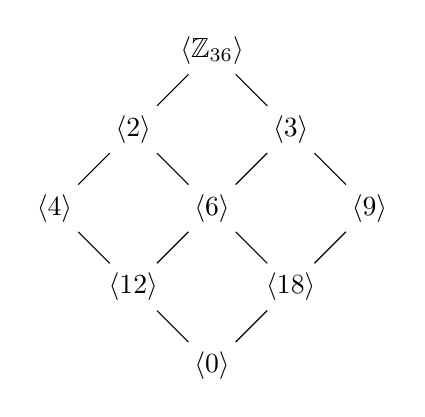
\begin{tikzpicture}[=>stealth]
\draw(0,0)node[]{$\langle 12\rangle$}
(1,1)node[]{$\langle 6\rangle$}
(2,2)node[]{$\langle 3\rangle$};
\draw(0.3,0.3)--(0.7,0.7)
(1.3,1.3)--(1.7,1.7);
\draw(0,2)node[]{$\langle 2\rangle$}
(1,3)node[]{$\langle \mathbb{Z}_{36}\rangle$}
(-1,1)node[]{$\langle 4\rangle$};
\draw(1,-1)node[]{$\langle 0\rangle$}
(2,0)node[]{$\langle 18\rangle$}
(3,1)node[]{$\langle 9\rangle$};
\draw(-0.7,1.3)--(-0.3,1.7)
(0.7,2.7)--(0.3,2.3);
\draw(-0.7,0.7)--(-0.3,0.3)
(0.3,1.7)--(0.7,1.3)
(1.3,2.7)--(1.7,2.3);
\draw(2.3,0.3)--(2.7,0.7)
(1.3,-0.7)--(1.7,-0.3)
(0.3,-0.3)--(0.7,-0.7)
(1.3,0.7)--(1.7,0.3)
(2.3,1.7)--(2.7,1.3);
\end{tikzpicture}
\end{figure}


















$\langle 2\rangle$ and $\langle 3\rangle$ are maximal ideals.

\item The ideal $\langle x^2 + 1\rangle$ is maximal in $\mathbb{R}[x]$. To show that this is the case, lets assume there is some ideal $A$ that properly contains $\langle x^2 + 1\rangle$. We show that $A = \langle x^2 + 1\rangle$. Thus $\langle x^2 + 1\rangle$ is maximal.\\\\
\end{enumerate}
\end{exa}






\begin{thm}
$R/A$ is an integral domain if and only if $A$ is prime.\\
\end{thm}

\begin{proof}
Suppose $R/A$ is an integral domain and $ab\in A$. Then $(a + A)(b + A) = ab + A  = A$, the zero elt of the ring $R/A$. So, either at $a + A = A$ or $b + A = A$. Thus either $a\in A$ or $b\in A\, \implies\, A$ is prime.\\
Conversely, suppose $R/A$ is a commutative ring with unity for any proper ideal $A$. We show that when $A$ is prime, $R/A$ has no zero division. Suppose $A$ is prime and $(a +A)(b + A) = 0 + A = A$. Then $a\in A$ therefore $a\in A$ and $b\in A$. Thus one of $(a + A) $ or  $(b + A)$ is the zero coset in $R/A$.\\\\
\end{proof}






\begin{thm}
$R/A$ is a field if and only if $A$ is maximal.\\
\end{thm}

\begin{proof}
Suppose $R/A$ is a field and $B$ is an ideal of $R$ that properly contains $A$. Let $b\in B,\, b\not\in A$. Then $b+A \neq 0$ in $R/A$ and therefore there exist an elt $c + A$ such that $(b + A)(c + A) = 1 + A$, the multiplicative identity of $R/A$. Since $b\in B$, we have $bc\in B$ since $1 + A = (b + A)(c + A) = bc + A$ so we have $1 - bc \in A\subset B$, so $1 = (1 - bc) + bc \in B$. Thus $B = R$ showing that $A$ is maximal.\\
Now, suppose $A$ is maximal and let $b\in R$ but $b\in\not A$. We show that $b + A$ does not have a multiplicative inverse. This follows from the fact that $A$ is a maximal ideal.\\\\
\end{proof}







\begin{defn}
Let $\phi : R \longrightarrow S$ be a ring homomorphism. Then the kernel of $\phi$ is $ker\, \phi = \{r\in R\, |\, \phi_r = 0\}$.\\


\textit{Image}\\
$Im \,\phi = \{s\in S\, |\, s = \phi_r$ for $r \in R\}$\\\\






\pagebreak
\end{defn}
\begin{thm}
For rings $R,\, S$ and a homomorphism $\phi : R\longrightarrow S$
\begin{enumerate}
\item $ker\, \phi$ is an ideal of $R$.
\item $Im\, \phi$ is a subring of $R$.
\item $Im\, \phi$ is isomorphic to the factor ring $R/ker\, \phi$.\\
\end{enumerate}
\end{thm}


\begin{proof}
\begin{enumerate}
\item Recall that $ker\, \phi \subset R$ is a subgroup under addition. Let $\, x\in ker\,\phi\,,\hspace{0.3cm} r\in R,\,\, r\in ker\,\phi$.

\item We just need to show that $Im\, \phi$ is closed under multiplication. $r_1, \, r_2 \in R$, then\\ $\phi(r_1)\,\phi(r_2) = \phi (r_1r_2)\in Im\, \phi$.\\\\\\
\end{enumerate}
\end{proof}












\subsection{Linear Operators (Transformation)}
Recall that a function takes a member and maps it to another number. But an operator maps a function to another.\\
E.G: $A = R[x]$. If $f\in A,\, D(f) = g(x) $ where $g = f'\,,\hspace{0.3cm} R[x] \longrightarrow R[x] \hspace{0.3cm} f\longmapsto g$.\\\\





\begin{defn}
A function $T: \mathbb{R}^n  \longrightarrow \mathbb{R}^m$ is said to be linear if:
\begin{enumerate}
\item[(i)]  for any $v,\, w\in \mathbb{R}^n\, ,\hspace{0.3cm} T(v + w) = T(v) + T(w)$
\item[(ii)] for any $v\in \mathbb{R}^n\, ,\hspace{0.2cm} \lambda \in \mathbb{R}\,,\, T(\lambda v) = \lambda T(v)$
\end{enumerate}
The map $T$ is often called a linear transformation or linear operator.\\

A number of properties from the definition.\\\\
\end{defn}




\begin{prop}
If $T: \mathbb{R}^n \longrightarrow \mathbb{R}^m$ is linear, then $T(O_{\mathbb{R}^n}) \longrightarrow O_{\mathbb{R}^m}$\\
\end{prop}


\begin{proof}
Consider the following equations $\, O_{\mathbb{R}^n}  + O_{\mathbb{R}^n} = O_{\mathbb{R}^n}$. Apply $T$ on both sides\\ $T(O_{\mathbb{R}^n} + O_{\mathbb{R}^n}) = T(O_{\mathbb{R}^n})$
\begin{align*}
\implies & T(O_{\mathbb{R}^n}) + T(O_{\mathbb{R}^n}) = T(O_{\mathbb{R}^n})\\\\
\implies &  T(O_{\mathbb{R}^n})  + T(O_{\mathbb{R}^n}) - T(O_{\mathbb{R}^n}) = T(O_{\mathbb{R}^n}) - T(O_{\mathbb{R}^n})\\\\
\implies & T(O_{\mathbb{R}^n}) = O_{\mathbb{R}^m}\\\\
\end{align*}







\vspace{2cm}
\end{proof}
\textbf{Examples}
\begin{enumerate}
\item The identity map $Id : \mathbb{R}^n \longrightarrow \mathbb{R}^n$ is a linear operator.\\

\textit{Check}: Let $u,\, v\in \mathbb{R}^n$
\begin{enumerate}
        \item[(i)] $Id (u + v) = u + v = Id(u) + Id (v)$
        \item[(ii)] $Id(\lambda u) = \lambda u = \lambda\, Id(u)$.\\
\end{enumerate}


\item Define $T: \mathbb{R}^3 \longrightarrow \mathbb{R}^3\,$ by $T\begin{pmatrix}
x\\
y\\
z\\
\end{pmatrix} = \begin{pmatrix}
x\\
y\\
-z\\
\end{pmatrix}$\\\\



\textit{Check}: Let $\, \begin{pmatrix}
x_1\\
y_1\\
z_1\\
\end{pmatrix}\, \hspace{0.2cm} , \, \hspace{0.2cm} \begin{pmatrix}
x_2\\
y_2\\
z_2\\
\end{pmatrix} \in \mathbb{R}^3$. Then 

\begin{enumerate}
\item[(i)] $T \begin{pmatrix}
\begin{pmatrix}
x_1\\
y_1\\
z_1\\
\end{pmatrix} + \begin{pmatrix}
x_2\\
y_2\\
z_2\\
\end{pmatrix}
\end{pmatrix}  = T \begin{pmatrix}
x_1 + x_2\\
y_1 + y_2\\
z_1 + z_2\\
\end{pmatrix} = \begin{pmatrix}
x_1 + x_2\\
y_1 + y_2\\
-(z_1 + z_2)\\
\end{pmatrix}  = \begin{pmatrix}
x_1\\
y_1\\
-z_1\\
\end{pmatrix} + \begin{pmatrix}
x_2\\
y_2\\
-z_2\\
\end{pmatrix}$\\\\

$ = T\begin{pmatrix}
x_1\\
y_1\\
z_1\\
\end{pmatrix} +  T\begin{pmatrix}
x_2\\
y_2\\
z_2\\
\end{pmatrix}$\\\\

\item[(ii)] For a scalar $\lambda$, $\, T\begin{pmatrix}
\lambda \begin{pmatrix}
x\\
y\\
z\\
\end{pmatrix}
\end{pmatrix} = T\begin{pmatrix}
\lambda\, x\\
\lambda\, y\\
\lambda\, z\\
\end{pmatrix} = \begin{pmatrix}
\lambda\, x\\
\lambda\, y\\
-\lambda\, z\\
\end{pmatrix} = \lambda\begin{pmatrix}
x\\
y\\
-z\\
\end{pmatrix} = \lambda\, T\begin{pmatrix}
x\\
y\\
z\\
\end{pmatrix}$\\\\
\end{enumerate}



\item Consider an operator of a transformation from $R[x]$ to $R[x]$ defined by $$T : \begin{pmatrix}
x_0\\
x_1\\
x_2\\
x_4\\
x_5\\
\end{pmatrix} \longmapsto \begin{pmatrix}
0\\
x_1\\
2 x_2\\
3x_3\\
4 x_4\\
\end{pmatrix}$$
Is this $T$ a linear transformation on $R[x]$?\\

\item The mapping $\, T: \mathbb{R}^2 \longrightarrow \mathbb{R}^2\,$ defined by $\, \displaystyle{T \binom{x}{y} = \binom{x}{x}}\,$ is linear.\\

\textbf{Proof}
\begin{enumerate}
\item[(i)] Let $\, \displaystyle{a = \binom{x_1}{y_1}\, , \, b = \binom{x_2}{y_2}\, , \hspace{0.3cm} a\, , \, b \in \mathbb{R}^2}$. Then
\begin{align*}
T(a + b) & = T\begin{pmatrix}
\begin{pmatrix}
x_1\\
y_1\\
\end{pmatrix} + \begin{pmatrix}
x_2\\
y_2\\
\end{pmatrix}
\end{pmatrix} = T \begin{pmatrix}
x_1 + x_2\\
y_1 + y_2\\
\end{pmatrix} = \begin{pmatrix}
x_1 + x_2\\
x_1 + x_2\\
\end{pmatrix}\\\\
& = \begin{pmatrix}
x_1\\
x_1\\
\end{pmatrix} + \begin{pmatrix}
x_2\\
x_2\\
\end{pmatrix} = T\binom{x_1}{y_1} + T\binom{x_2}{y_2}\\\\
& = T(a) + T(b)
\end{align*} 

\item[(ii)] for $\, \lambda\in \mathbb{R}$, we have $T(\lambda \, a) = T\begin{pmatrix}
\lambda\, x_1\\
\lambda\, y_1\\
\end{pmatrix} = \begin{pmatrix}
\lambda\, x_1\\
\lambda\, x_1\\
\end{pmatrix} = \lambda \begin{pmatrix}
x_1\\
x_1\\
\end{pmatrix} = \lambda \, T\begin{pmatrix}
x_1\\
y_1\\
\end{pmatrix} = \lambda \, T(a)$\\

$\therefore\, T$ as defined is linear.\\\\
\end{enumerate}



\item $T : \mathbb{R}^2 \longrightarrow \mathbb{R}^2\,$ defined by $\, \displaystyle{\binom{x}{y} \longmapsto \binom{x - 1}{y - 1}}\,$ is not linear.\\\\


Let $\, \displaystyle{a = \binom{x_1}{y_1}\, \hspace{0.3cm} , \, \hspace{0.3cm} b = \binom{x_2}{y_2}\, , \hspace{0.3cm} a\, ,\, b \in \mathbb{R}^2}$. Then 
\begin{align*}
T(a + b) & = T\begin{pmatrix}
x_1 + x_2\\
y_1 + y_2\\
\end{pmatrix} = \begin{pmatrix}
x_1 + x_2 - 1\\
y_1 + y_2 - 1\\
\end{pmatrix} = \begin{pmatrix}
x_1\\
y_1\\
\end{pmatrix} + \begin{pmatrix}
x_2 - 1\\
y_2 - 1\\
\end{pmatrix}\\\\
& \neq \begin{pmatrix}
x_1 - 1\\
y_1 - 1\\
\end{pmatrix} + \begin{pmatrix}
x_2 - 1\\
y_2 - 1\\
\end{pmatrix} = T\begin{pmatrix}
x_1\\
y_1\\
\end{pmatrix} + T\begin{pmatrix}
x_2\\
y_2\\
\end{pmatrix} = T(a) + T(b)
\end{align*}
$\therefore\, T $ is not linear.\\\\



\item $T : \mathbb{R}^2 \longrightarrow \mathbb{R}^2\,$ defined by $\displaystyle{\binom{x}{y} \longmapsto \binom{x}{x^2}}\,$ is not linear.\\\\\


\begin{proof}
Let $\, a\, ,\, b\in \mathbb{R}^2\,$ such that  $\, \displaystyle{a = \binom{x_1}{y_1}\, \hspace{0.3cm},\hspace{0.3cm} b = \binom{x_2}{y_2}}$. Then
\end{proof}
\begin{align*}
T(a + b) & = T\begin{pmatrix}
x_1 + x_2\\
y_1 + y_2\\
\end{pmatrix} = \begin{pmatrix}
x_1 + x_2\\
x_1^2 + x_2^2 + 2x_1x_2\\
\end{pmatrix}\\\\
& \neq \begin{pmatrix}
x_1 + x_2\\
x_1^2 + x_2^2\\
\end{pmatrix} = \begin{pmatrix}
x_1\\
x_1^2\\
\end{pmatrix} + \begin{pmatrix}
x_2\\
x_2^2\\
\end{pmatrix} = T\binom{x_1}{y_1} + T{x_2}{y_2} = T(a) + T(b)
\end{align*} 
$\therefore\, T$ as defined is not linear.\\\\\\
\end{enumerate}








\begin{exa}
Let $A$ be an $m\times n$ matrix. Then $A$ defines a linear map $\, L_A : \mathbb{R}^n \longrightarrow \mathbb{R}^m$ $(``$ left multiplication by $A")$ denoted by $\, L_A(v) = A_v,\, $ for $\, v\in \mathbb{R}^n$.\\\\
\end{exa}







\begin{thm}[Recall the fundamental Homomorphism]
$\phi : G \longrightarrow H, \, G$ and $H$ groups, $\, \, G\big/ker\, \phi\, \cong\, H$.\\
\end{thm}






\begin{proof}
Since $ker\, \phi$ is an ideal of $R,\hspace{0.2cm} R/ker\, \phi\,$ is a ring. Recall that a  ring is a group under addition. $Im\, \phi$ is also a subring thus it is a group under addition.\\
Now, define a map $\, h = R/ker\, \phi \longrightarrow Im\, \phi$.\\
$k + R \, \longrightarrow \, \phi (R)$.\\
We check that indeed $h$ as defined respects the map operations. let $k_1 + R$ and $k_2 + R$ be in $\, R/ker\, \phi$
\begin{align*}
h(k_1 + R)(k_2 + R) & = h(k_1k_2 + k_1R + Rk_2  + R)\\
& = h(k_1k_2 + R)\\
& = \phi (R)
\end{align*}
Clearly, $h$ is well behaved. We involve the fundamental homonorphism theorem, we have that $h$ is a isomorphism and therefore $\, R/\ker\, \phi \cong Im\, \phi$.\\














\pagebreak
\end{proof}
\section{INTRODUCTION TO MODULES}
A module  is a generalization of a vector space. Instead of a vector space of a field, we consider one over a ring.\\\\



\begin{defn}
A left $R-$module $M$ over a ring $R$ with unity $1_R$ is a abelian group with scalar product\\ $\, \bullet : R \times M \, \longrightarrow \, M$. We write $\, \bullet\, (\alpha , m) = \alpha m$ defined for all $\alpha \in R,\, m\in M\,$ satisfying the following axioms:
\begin{enumerate}
\item[(i)] $\alpha \, \cdot\, (\beta\cdot m) = (\alpha \beta)\cdot m$
\item[(ii)] $(\alpha + \beta ) \cdot m = \alpha \cdot m + \beta \cdot m$
\item[(iii)] $\alpha \cdot (m + n) = \alpha \cdot m  + \alpha \cdot n$
\item[(iv)] $1_R\cdot m = m$ where $\alpha,\, \beta \in R,\,\, m,\, n\in M$.
\end{enumerate}

A similar definition exists for Right $R-$module!\\\\
\end{defn}



\textbf{Example}
\begin{enumerate}
\item Let $R = \mathbb{Z}$. Then if $M$ is any abelian group. We may define a $\mathbb{Z}-$module structure on $M$ as follows $\, (n,x) \longmapsto nx$\\
\textit{Check} that for $n_1,\, n_2\in \mathbb{Z},\,\, x,\, y\in M $
\begin{enumerate}
      \item[(i)] $n_1\cdot (n_2\cdot x) = n_1 n_2 x$
      \item[(ii)] $(n_1 + n_2)\cdot x = n_1\cdot x + n_2\cdot x$
      \item[(iii)] $n_1\cdot (x+ y) = n_1\cdot x + n_1 \cdot y$
      \item[(iv)] $1_R\cdot x = 1\cdot x = x$\\
\end{enumerate}



\item Let $R = K$ field. Then the module over $K$ is  a vector space. Many facts about vector spaces remain true for modules. e.g consider $a\neq 0$ in a field $K$, then $\, ax = 0\, \implies \, x = 0$. But this is not true in general for any module.


\item Let $R$ be a ring. Consider then multiplication $\, \bullet\, R\times R \longmapsto R$. This defines a  module structure on the ring $R$. This is both a right and left $R-$module.


\item Let $K$ be a field and let $R = M_n(K)$ be the ring of $n\times n$ matrices over the field $K$. Let $M = K^n$ visualized as a column vector of $n$ entries.
$$R\times M \longmapsto M$$
$$(a,x) \longmapsto ax$$

$$a = \begin{pmatrix}
a_{11} & \cdots\cdots & a_{1n}\\
a_{21} & \cdots\cdots & a_{2n}\\
\vdots &              & \vdots\\
\vdots &              & \vdots\\
a_{n1} & \cdots\cdots & a_{nn}\\
\end{pmatrix} \hspace{0.5cm},\hspace{0.5cm}
x = \begin{pmatrix}
x_1\\
\vdots\\
\vdots\\
x_n\\
\end{pmatrix}$$\\



$$(a,x) = \begin{pmatrix}
\begin{pmatrix}
a_{11} & \cdots\cdots & a_{1n}\\
a_{21} & \cdots\cdots & a_{2n}\\
\vdots &              & \vdots\\
\vdots &              & \vdots\\
a_{n1} & \cdots\cdots & a_{nn}\\
\end{pmatrix} \hspace{0.2cm},\hspace{0.2cm}
\begin{pmatrix}
x_1\\
\vdots\\
\vdots\\
x_n\\
\end{pmatrix}
\end{pmatrix}$$\\



$$ ax = \begin{pmatrix}
a_{11} x_1 + a_{12} x_2  + \, \cdots\cdots \, + a_{1n} x_n\\
\vdots\\
\vdots\\
a_{n1} x_1 + a_{n2} x_2 + \, \cdots\cdots \, + a_{nn} x_n\\
\end{pmatrix}$$



\item Let $R$ be a ring and $n$ a rational number, the Cartesian product $R^n$ is both a left and Right $R-$module (If we use component-wise operation).

\item Let $S$ be a non-empty set, $M$ a left $R-$module, and $M^s = \{ f: s\longrightarrow M\}$. Define addition and multiplication as follows:
$$(f  + g) (s) = f(s) + g(s)\,\hspace{0.4cm} ,\hspace{0.4cm} \, (rf) (s) = r\big(f(s)\big)$$
The $M^2$ is a left $R-$module.\\

\textit{Check}\\
Let $f,\, g\in S\, ,\hspace{0.2cm} s,\, t\in M\,$ then $M^s$ satisfies:
\begin{enumerate}
    \item[(i)] $f\cdot (g\cdot s) = f\cdot (g(s)) = (fg) (s) = (fg)\cdot s$
    \item[(ii)] $(f + g)\cdot s = (f + g)\cdot s = f\cdot s + g\cdot s = f(s) + g(s)$
    \item[(iii)] $f\cdot (s + t) = f\cdot s + f\cdot t = f(s) + f(t)$
    \item[(iv)] $1_R\cdot s = 1\cdot s = 1(s) = s$\\
\end{enumerate}



\item Let $X$ be a  $\underbrace{\text{Smooth}}_{\text{(inifitely differentiable)}}$ $\,$ manifold$(\mathbb{R}^2 = (x,y) $ a surface in $2-D)$\\

Sphere: \hspace{0.3cm} $\begin{vmatrix}
z\\
\end{vmatrix} = R\hspace{0.3cm}, \hspace{0.3cm} \sqrt{x^2 + y^2 + z^2} \, = r\hspace{0.3cm} (x, y , r)\longmapsto r$\\
Then consider the smooth functions on $X$ to real numbers. This set of smooth functions, form a ring $C^{\infty} (X)$.  The set of all smooth vectors fields defined on $X$ is module over $C^{\infty}(X)$.\\\\



\textbf{Assignment}\\
Check that indeed the vector field $\overrightarrow{\nabla}\, f$ forms a module over the ring of functions\\ $\, f: x \longrightarrow \mathbb{R}$. $($ Take $X=\mathbb{R}^3)$, where
$$\overrightarrow{\nabla} f = \frac{\partial f}{\partial x} \, \textbf{i} + \frac{\partial f}{\partial y}\, \textbf{j} + \frac{\partial f}{\partial z}\, \textbf{k}$$


\item If $R$ is a ring, define $R^{op}$ with elements as in $R$, but multiplication defined as follows: If $ab = c$, then $ba = c \in  R^{op}$. Any left $R-$module $M$ can be seen as the right module over $R^{op}$.
\end{enumerate}











\subsection{Submodules}

\begin{defn}
Let $M$ be a left $R-$module and $N$ a subgroup of $M$. Then $N$ is a submodule (or $R-$ submodule) if for any $n\in \mathbb{N}$ and any $r\in R,\hspace{0.3cm} rn\in N$.\\

\textit{Note:} Given a module $M$, the set of all submodules of $M$ forms a lattice that satisfies the \underline{modular law}.\\\\
\end{defn}


\textbf{Modular Law}\\
Given submodules $U, \, N_1,\, N_2$ of $M$ such that $N_1\subset N_2$, then $\, \big(N_1 + U\big) \cap N_2 = N_1 + \big(U \cap N_2\big) $.\\\\


\begin{defn}
Let $M$ and $N$ be modules the map $f: M\longrightarrow N$ is a homomorphism of modules if for any $m,\, n \in M$ and $r,\, s\in R,$ $$ f(rm + sn) = r\, f(m) + s\, f(n)$$

$-$ This is sometimes called an \underline{$R-$ linear map}.\\
$-$ A bijective module homomorphism is called \underline{isomorphism of modules}.\\\\\\
\end{defn}





\textbf{Types of Modules}
\begin{enumerate}
\item \textit{Cyclic module:}  A module generate by a single elements.
\item \textit{Finitely generated:}  A module generated by a finite number of elements.
\item \textit{Free module:} A module that has a basis or one which is isomorphic to some direct sum of some copies of $R$.
\item \textit{Projective modules:} Are direct summands of free modules.
\item \textit{Injective modules:} Duals of projective modules.
\item \textit{Faithful module:} $M$ is faithful if the action of each $r\neq 0$ in $R$ on $M$ in nontrivial (i.e, $rx\neq 0$ for some $x\in M$).\\\\
\end{enumerate}






\pagebreak
\section{FIELD EXTENSIONS}

\textbf{Motivation}\\
Recall that for a quadratic with discriminant $\, b^2 - 4ac < 0$. We started (in high school) by stating it as not having a solution. Then described it having no real roots.\\


Consider $\, 1 + 3\sqrt{2}  = -1 + 3\sqrt{2}  + (\sqrt{2})^2 \in \mathbb{Q}[\sqrt{2}\,]$.\\

But $\, 1 + 3x \neq -1 + 3x + x^2 \in Q [x]$.\\\\



\begin{defn}
Let $E$ be a field containing a subfield $F$. Then $E$ said to be an extension of the field $F$ denoted $E/F$ .  Read as ``$E$ over $F$".\\\\
\end{defn}


\begin{defn}
The degree of a field extension $E/F$ denoted as $[E:F]$ is dimension of $E$ as a vector space over $F$.\\



$\bullet$ If $[E:F]$ is finite, then the extension is of finite index $X$. Otherwise it is said to be infinite.\\\\
\end{defn}


\begin{exa}
Consider the field $\mathbb{Q}\, , \,\, p(x)  = x^2 - 2\in \mathbb{Q}[x]$. But the roots $\pm \sqrt{2}\, \in \mathbb{Q}$. Clearly, $p(x)$ has no solutions in $\mathbb{Q}[x]$. We say $p(x) = x^2 - 2$ is irreducible over $\mathbb{Q}$.\\
We would like to extend $\mathbb{Q}$ so that it includes the roots for $p(x) = x^2 - 2$.\\
Consider the following quotient ring $\, \mathbb{Q}[x]/x^2 - 2  = \{q(x) + \langle x^2 - 2\rangle\, |\, q(x)\in \mathbb{Q}[x]\}$.\\

We can show that $\, \mathbb{Q}[x]/x^2 - 2 \cong \mathbb{Q}[\sqrt{2}]$\\\\


$\bullet$ Take the field $\mathbb{R}$, a polynomial like $\, p(x) = x^2 + 1 \in R[x]$ is irreducible over $\mathbb{R}$. It is obvious that the roots $\, \pm i \not\in \mathbb{R}$. Thus if we consider the quotient: $\, \mathbb{R}[x]/x^2 + 1 \cong \mathbb{R}[i] \cong \mathbb{C}$.\\\\
\end{exa}




\begin{thm}[Fundamental Theorem of Field Theory]
Let $F$ be a field and $f(x)$ be a non-constant function in $F[x]$. Then there is an extension $E$ of $F$ such that $f(x)$ has a zero in $E$.\\\\
\end{thm}





\begin{exa}
\begin{enumerate}
\item Let $\, f(x) = x^2 + 1 \in \mathbb{Q}[x]$, then in $\, E = \,\mathbb{Q}[x]\big/(x^2 + 1)\,  \cong \,\mathbb{Q}[i]$
\begin{align*}
f(x + \langle x^2 + 1\rangle ) & = (x + \langle x^2 + 1\rangle )^2 + 1\\
& = x^2 + x\cdot \langle x^2 + 1\rangle + \langle x^2 + 1\langle\cdot x + \langle x^2 + 1\rangle^2 + 1\\
& = x^2 + 1 + \langle x^2 + 1\rangle\\
& = 0 + \langle x^2 + 1\rangle
\end{align*}
$*$ What conclusion can you make?\\
The explanation is that in $\mathbb{Q}[x]\, ,\, \, x^2 + 1\,$ can be a zero.\\



\item Let $f(x) = x^5  - 2x^2 + 2x + 2\in \mathbb{Z}_3[x]$. Then the irreducible factorization of $f(x)$ over $\mathbb{Z}_3$ is $(x^2 + 1)(x^3 + 2x + 2)$. So, to extend $\mathbb{Z}_3$ to a field $E$ in which $f(x)$ has a zero, we may take. $$E = \,\mathbb{Z}_3[x]\big/\langle x^2 + 1\rangle\hspace{0.6cm} (\text{pick any of the two factors}).$$



\textit{Check}
\begin{align*}
f(x + \langle x^2 + 1\rangle ) & = (x + \langle x^2 + 1\rangle )^5 - 2(x + \langle x^2 + 1\rangle)^2 + 2(x + \langle x^2 + 1\rangle) + 2\\
& = x^5 + \langle x^2 + 1\rangle^5 - 2x^2 - 2\langle x^2 + 1\rangle^2 + 2x + 2\langle x^2 + 1\rangle + 2\\
& = x^5 - 2x^2  + 2x + 2 + \langle x^2 + 1\rangle^5\\
& = (x^2 + 1)(x^3 + 2x + 2) + \langle x^2 + 1\rangle^5\\
& = (x^3 + 2x + 2) + \langle x^2 + 1\rangle^5\\\\
\end{align*}


or $\hspace{0.3cm} E = \mathbb{Z}_3[x]\big/\langle x^3 + 3x + 2\rangle$\\\\



\textit{Check}
\begin{align*}
f(x + \langle x^3 + 2x + 2\rangle) & = (x + \langle x^3 + 2x + 2\rangle)^5 - 2(x + \langle x^3 + 2x + 2\rangle)^2 + 2(x + \langle x^3 + 2x + 2\rangle) + 2\\
& = x^5 + \langle x^3 + 2x + 2\rangle^5 - 2x^2 - \cancel{2\langle x^3 + 2x + 2\rangle^2} + 2x + \cancel{2\langle x^3 + 2x + 2\rangle^2} + 2\\
& = x^5 - 2x^2 + 2x + 2 + \langle x^3 + 2x + 2\rangle\\
& = (x^2 + 1)(x^3 + 2x + 2) + \langle x^3 + 2x + 2\rangle\\
\end{align*}



\item Let $f(x) = 2x + 1 \in \mathbb{Z}_4[x]$ has no solution in $\mathbb{Z}_4[x]$ since $x = -1/2$ and\\ $\, -1/2 = a$ mod$_4 \, \implies \, 3 = 2a$ mod$_4$. Thus there is no $a\in \mathbb{Z}_4$ that satisfies the equality.\\
$$E = \mathbb{Z}_4[x]\big/\langle 2x + 1\rangle$$

So that $\, f(x) = 2x + 1\, $ has a solution in $\, \mathbb{Z}_4[x]\big/\langle 2x + 1\rangle$
\begin{align*}
f(x  + \langle 2x + 1\rangle ) & = 2(x + \langle 2x + 1\rangle) + 1\\
& = 2x + 1 2\langle 2x + 1\rangle\\
& = 0 + \langle 2x + 1\rangle
\end{align*}

$\therefore\, 2x + 1$ is the  zero in $\mathbb{Z}_4[x]$.\\\\\\
\end{enumerate}





\pagebreak
\end{exa}
\textbf{Factorization of Polynomials}\\


\begin{defn}
Let $D$ be an integral domain. A polynomial $f(x)$ in $D[x]$ that is neither zero or a unity in $D[x]$ is said to be irreducible over $D$ if whenever $f(x)$ is expressed as a product $g(x)\, h(x)$, where $g(x)\, ,\, h(x)\in D[x]$, then $h(x)$ or $g(x)$ is a unity in $D[x]$.\\\\
\end{defn}


\begin{exa}
\begin{enumerate}
\item The polynomial $\, f(x) = 2x^2 + 4\,$ is irreducible over $\mathbb{Q}$, but is reducible over $\mathbb{C}$.

\item The polynomial $\, f(x) = x^2 - 2\,$ is reducible over $\mathbb{R}$ but irreducible over $\mathbb{Q}$.\\\\
\end{enumerate}
\end{exa}





\textbf{Theorem. (Irreducibility Test) ``for degree 2 and 3"}\\
Let $F$ be a field. If $f(x)\in F[x]$ and degree of $f(x)$ is 2 or 3, then $f(x)$ is reducible over $F$ if and only if $f(x)$ has a zero in $F$.\\

\begin{proof}
Suppose $f(x) = h(x)\, g(x)$, where both $h(x)\, , g(x)\in F(x)$ and have deg less than that of $f(x)$. Then $$\deg (f(x)) = \deg (h(x)) + \deg (g(x))\hspace{0.3cm}\text{and}\hspace{0.3cm} \deg (f(x))$$
at least one of  $h(x)$ and $g(x)$ has degree 1. Say $g(x) = ax + b$. Thus clearly $-a^{-1}b$ is a zero for $f(x)$.\\
Conversely, suppose $f(a) = 0$ for some $a\in F$, then by the factor theorem, we know that $(x - a)$ is a factor of $f(x)$ then $f(x)$ is reducible over $F$.\\\\
\end{proof}





\begin{defn}
The content of a non zero polynomial $\, a_n x^n + a_{n-1} x^{n - 1} + \cdots\cdots + a_0$, where the $a_i \in \mathbb{Z}$ is the $g\subset d $ of $a_n\, ,\, a_{n-1}\, , \, \cdots\cdots, a_0$.\\
In the case where the content is equal to 1 for a polynomial over $\mathbb{Z}[x]$, then the polynomial is said to be primitive.\\\\
\end{defn}






\textbf{Lemma [Gauss]}\\
The product of two primitive polynomials is primitive.\\

\begin{proof}
Let $f(x)$ and $g(x)$ be primitive. Suppose that the product $f(x)\,g(x)$ is not primitive. Then the content of $f(x)\, g(x) \neq 1$. Let $p$ be a prime divisor of the content of $f(x)\, g(x)$. Let $\overline{f(x)}\, , \, \overline{g(x)}$ and  $\overline{f(x)\, g(x)}$ be polynomials obtained from $f(x)\, , \, g(x)$ and $f(x)\, g(x)$ mod$_p$. Then $\overline{f(x)}$ and $\overline{g(x)}$ belong to the integral domain $\mathbb{Z}_p[x]$.\\
Now $\, \overline{f(x)}\, \,\overline{g(x)}  = \overline{f(x)\, g(x)} = 0\,$ in $\mathbb{Z}_p[x]$. Thus $\overline{f(x)} = 0$ or $\overline{g(x)} = 0$. This means that either $p$ divides every coefficient of $f(x)$ or $p$ divides every coefficient of $g(x)$. Hence either $f(x)$ is not primitive or $g(x)$ is not primitive. This is a contradiction.\\\\
\end{proof}





\begin{thm}[Irreducibility over $\mathbb{Q}$ implies over $\mathbb{Z}$]
Let $f(x)\in \mathbb{Z}[x]$. If $f(x)$ is irreducible over $\mathbb{Q}$, then it is irreducible over $\mathbb{Z}$.\\
\end{thm}

\begin{proof}
Suppose $\, f(x) = g(x)\, h(x)\,$ where $g(x)\, , \, h(x)\in \mathbb{Q}[x]$. Clearly, we assume $f(x)$ is primitive since we can divide both $f(x)$ and $g(x)\, h(x)$ by the content of $f(x)$. Let  $a$ be the $L\subset M$ of the denominators of the coefficients of $g(x)$ and $b$ the $LCM$ of the denominators of $h(x)$. Then
$$a\, b\, f(x) = a\, b \cdot g(x)\, h(x) = a\, g(x) \cdot b\, h(x)$$
where $a\, g(x)$ and $b\, h(x)$ are in $\mathbb{Z}[x]$. Let $c_1$, be the content of $a\, g(x)$ and $c_2$ be the content of $b\, h(x)$. Then $a\, g(x) = c_1\, g_1(x)$ and $b\, h(x) = c_2\, h_1(x)$ where both $g_1(x)$ and $h_1(x)$ are primitive and  $a b f(x) = c_1 c_2\, g_1(x)\, h_1(x)$. Since $f(x)$ is primitive then content of $ab\, f(x)$, it follows that the content of  $c_1 c_2\, g_1(x)\, h_1(x)$ is $c_1 c_2$. Thus $a b = c_1 c_2$ and $f(x) = g_1(x)\, h_1(x)$ where $g_1(x)$ and $h_1(x)\in \mathbb{Z}[x]$ and $\deg g_1(x) = \deg g(x)$. $\, \deg h_1(x) = \deg h(x)$.\\\\
\end{proof}






\begin{thm}[mod$_p$ Irreducibility test]
Let $p$ be a prime and suppose $f(x)\in \mathbb{Z}[x]$ with $\deg f(x) \geq 1$. Let $\overline{f(x)}$ be the polynomial obtained from $f(x)$ by taking coefficients mod$_p$. $\, \overline{f(x)}\in \mathbb{Z}_p[x]$. If $\overline{f(x)}$ is irreducible over $\mathbb{Z}_p[x]$ and $\deg \overline{f(x)} = \deg f(x)$, then $f(x)$ is irreducible over $\mathbb{Q}$.\\
\end{thm}


\begin{proof}
If $f(x)$ is reducible, then $f(x) = g(x)\, h(x)$ where $g(x)\, , \, h(x)\in \mathbb{Z}[x]$ and are of degree less than $f(x)$.\\
Now, $\deg \overline{f(x)} = \deg f(x)$. Thus, we have $\deg \overline{g(x)} \leq \deg g(x) < \deg \overline{f(x)}$ and $\deg \overline{h(x)} \leq \deg h(x) < \deg \overline{f(x)}$. But $\overline{f(x)} = \overline{g(x)}\, \overline{h(x)}$ and this is a contradiction to our assumption that $\overline{f(x)}$ is irreducible over $\mathbb{Z}_p$.\\\\
\end{proof}



\textbf{Example}
\begin{enumerate}
\item $f(x) = 21x^3 - 3x^2 + 2x + 9\, $ let $p = 2$, then $\overline{f(x)}  = x^3 - x^2 + 1\hspace{0.3cm} \deg \overline{f(x)} = \deg f(x)$ and $\overline{f(0)} = 1\, , \hspace{0.3cm} \overline{f(1)} = 1,\,$ we see that $\overline{f(x)}$ is irreducible over $\mathbb{Z}_2$. Thus $f(x)$ is irreducible over $\mathbb{Q}$.\\


\item Let $f(x) = \dfrac{3}{7}\, x^4 - \dfrac{2}{7}\, x^2 + \dfrac{9}{35}\, x + \dfrac{3}{5}\,$ show that $f(x)$ is irreducible over $\mathbb{Q}$.\\

\begin{solution}
Let $\, h(x) = 35\, f(x) = 15x^4 - 10 x^2 + 9x + 21$. Choose $p = 2$. $\overline{h(x)} = x^4 + x + 1\hspace{0.3cm}$\\
\end{solution}

$ \deg \overline{h(x)} = \deg h(x)$.
\begin{align*}
\overline{h(0)} & = 1 \neq 0\\
\overline{h(1)} & = 1 \neq 0
\end{align*}
$\therefore\,\overline{h(x)}$ is irreducible in $\mathbb{Z}_2[x]$, hence by our theorem, $h(x)$ is irreducible over $\mathbb{Q}$. Since $h(x) = 35\, f(x)$, we have that $f(x)$ is also irreducible over $\mathbb{Q}$.\\

\item Show that $f(x)  = x^5 + 2x + 4$ is irreducible over $\mathbb{Q}$.\\




\pagebreak
\textbf{Solution}\\
Let $p = 2$ so that $\overline{f(x)} = x^5\, ,\hspace{0.3cm} \overline{f(0)} = 0\, , \hspace{0.3cm} \overline{f(1)} = 1 \neq 0$ so that or let $p = 3$,\\$\hspace{0.3cm} \overline{f(x)} = x^5 + 2x + 1\, \implies\, \overline{f(0)} = 1\, , \hspace{0.3cm} \overline{f(1)} = 1\, , \hspace{0.3cm} \overline{f(2)} = 1$\\
$\therefore\,\overline{f(x)}$ is irreducible over $\mathbb{Z}_3[x]\, \implies\, f(x) $ is irreducible over $\mathbb{Q}$.\\\\
\end{enumerate}







\textbf{Eisenstein Criterion}\\
Let $f(x) = a_n x^n + a_{n-1} x^{n-1}  + \cdots\cdots + a_0 \in \mathbb{Z}[x]$. If there is a prime $p$ such that\\ $p \dagger a_n\, , \hspace{0.3cm} p\, |\, a_{n - 1}\, , \, a_{n-2}\, , \, \cdots\cdots, a_0$ and $p^2\dagger a_0$ , then $f(x)$ is irreducible over $\mathbb{Q}$.\\\\





\textbf{Corollary Eisenstein's [Irreducibility of $p^{\text{th}}$ cyclotomic polynomial]}\\
For any prime $p$, the $p^{\text{th}}$  Cyclotomic polynomial; $$ \Phi_p(x) = \frac{x^p - 1}{x - 1} = x^{p - 1} + x^{p - 2} + x^{p - 3} + \cdots\cdots\cdots + 1$$ is irreducible over $\mathbb{Q}$.\\


\begin{proof}
$$f(x) = \Phi_p(x + 1) = \dfrac{(x + 1)^p - 1}{(x + 1) - 1} = (x + 1)^{p - 1} + (x + 1)^{p -2} + \cdots\cdots\cdots + 1 = x^{p-1} + p\, x^{p-2} + \cdots\cdots\cdots + 1\hspace{0.3cm} (*)$$
Then, since every coefficient of $x^{p - 1}$ is divisible by $p$ by Eisenstein's Criterion, $f(x)$ is irreducible over $\mathbb{Q}$. So if $\Phi_p(x) = g(x)\, h(x)$ was some non-trivial factorization of $\Phi_p(x)$, then\\ $f(x) = \Phi(x + 1) = g(x + 1)\, h(x + 1)$ would be a nontrivial factorization of $f(x)$ over $\mathbb{Q}$.
Now since this is impossible, we conclude that $\Phi_p(x)$ is irreducible.\\\\
\end{proof}





\begin{exa}
The polynomial $\, 3x^5 + 15x^4 - 20x^3 + 10x + 20\, $ is irreducible over $\mathbb{Q}$ because $\, 5\dagger 3\, , \hspace{0.3cm} 5^2\dagger 20\,$ but $5\, |\, 15\, , \, -20\, , \, 10\, , \, 20$. Thus the polynomial is irreducible over $\overline{Q}$.\\\\
\end{exa}




\begin{thm}
$p(x)$ is irreducible if and only if $\langle p(x)\rangle $ is maximal.\\

$\bullet\,$ Let $\mathbb{F}$ be a field, and let $p(x) \in \mathbb{F}[x]$. Then $\langle p(x) \rangle$ is a maximal ideal in $\mathbb{F}[x]$ if and only if $p(x)$ is irreducible over $\mathbb{F}$.\\
\end{thm}


\begin{proof}
Suppose that $\langle p(x)\rangle$ is maximal in $\mathbb{F}$. Clearly, $\langle p(x)\rangle$ is neither the zero nor the 1 in $\mathbb{F}$. If $p(x) = g(x)\, h(x)$ is a factorization of $p(x)$ over $\mathbb{F}[x]$. Then $\langle p(x) \rangle \subseteq \langle g(x)\rangle \subseteq \mathbb{F}$. But since $\langle p(x)\rangle$ is maximal then $\langle p(x)\rangle = \mathbb{F}$. (Since it implies $\langle p(x) \rangle = \langle g(x)\rangle)$. Thus deg $p(x) = \deg g(x)$, hence $\deg h(x) = 0$. Thus $p(x)$ cannot be written as a product of polynomials of lower degree in $\mathbb{F}[x]$.\\
Conversely, suppose $p(x)$ is irreducible over $\mathbb{F}$. Let $I$ be any ideal of $\mathbb{F}[x]$ such that $\langle p(x) \rangle \subseteq I \subseteq \mathbb{F}[x]$. Now, $\mathbb{F}[x]$ is a principle ideal domain, we have $I = \langle g(x)\rangle$ for some $g(x)\in \mathbb{F}[x]$. So, $p(x)\in \langle g(x)\rangle$. Hence $p(x) = g(x)\, h(x)$, where $h(x)\in \mathbb{F}[x]$. Now, since $p(x)$ is irreducible over $\mathbb{F}$, it follows that $g(x)$ or $h(x)$ is constant. In this case, we have $I = \mathbb{F}[x]$ or $\langle p(x) \rangle = \langle g(x)\rangle = I$. Thus $\langle p(x)\rangle$ is maximal in $\mathbb{F}[x]$.\\\\
\end{proof}









\begin{thm}
$\Big(\mathbb{F}[x]/\langle p(x)\rangle$ is a Field$\Big)$.\\
Let $\mathbb{F}$ be a field and $p(x)$ on irreducible polynomial over $\mathbb{F}$, then $\mathbb{F}[x]/\langle p(x)\rangle\, $ is a field.\\\\
\end{thm}

\begin{proof}
$\mathbb{F}[x]$ is a commutative ring with identity, so the quotient by an ideal
is a commutative ring with identity. It remains to produce inverses.

Let $g(x) + \langle p(x)\rangle$ be a non-zero coset, so $p \nmid g$. Since $p$
is irreducible, its only divisors are units and associates of itself, so
$\gcd(p,g) = 1$. By the division algorithm in $\mathbb{F}[x]$ there are $u,v$
with
$$u(x)p(x) + v(x)g(x) = 1 ,$$
and reducing modulo $\langle p(x)\rangle$ gives
$v(x)g(x) \equiv 1$. So $v(x)+\langle p(x)\rangle$ is the required inverse, and
the quotient is a field.
\end{proof}

\begin{note}
Irreducibility is exactly what is needed. If $p$ factors as $p = p_1p_2$ with
both factors of positive degree, then the non-zero cosets of $p_1$ and $p_2$
multiply to zero, so the quotient has zero divisors and cannot be a field. This
is the polynomial mirror of $\mathbb{Z}_n$ being a field precisely when $n$ is
prime.
\end{note}




\begin{coro}
$\Big(p(x)\, |\, a(x)\, b(x)\, $ implies that $p(x)\, |\, a(x)$ or $p(x)\, |\, b(x)\Big)$\\
Let $\mathbb{F}$ be a field and let $p(x)\, , \, a(x)\, , \, b(x)\in \mathbb{F}[x]$. If $p(x)$ is irreducible over $\mathbb{F}$ and $p(x)\, |\, a(x)\, b(x)$, then $p(x)\, |\, a(x)$ or $p(x)\, | \, b(x)$.\\
\end{coro}

\begin{proof}
Suppose $p(x)$ is irreducible, then $\mathbb{F}/\langle p(x)\rangle$ is a field thus it is an integral domain. Let $\overline{a}(x)$ and $\overline{b}(x)$ be the images of the natural homomorphism of $a(x)$ and $b(x)$. Now, since $p(x)\, |\, a(x)\, b(x)$, we have $\overline{a}(x)\, \overline{b}(x) = \overline{0}$, then zero in $\mathbb{F}/\langle p(x) \rangle$. Thus $\overline{a}(x) = \overline{0}$ or $\overline{b}(x) = \overline{0}$ and it follows that $p(x)\, |\, a(x)$ or $p(x)\, |\, b(x)$.\\\\\\\\
\end{proof}







\textbf{Splitting Fields}\\

\begin{defn}
Let $E$ be a field extension of a field $F$ and $f(x)\in F[x]$. Then $f(x)$ splits in $E$ if $f(x)$ can be factored as a product of linear factors in $E[x]$.\\

$\bullet$ We call $E$ a splitting field for $f(x)$ over $F$ is $f(x)$ splits in $E$  but in proper sub field  of $E$.\\\\
\end{defn}





\begin{exa}
Let $f(x) = x^2 + 1$ in $\mathbb{Q}[x]$. Since $x^2 + 1 = \big(x + \sqrt{-1}\big)\big(x - \sqrt{-1}\big)$, we see that $f(x)$ splits in $\mathbb{C}$ but a splitting field over $\mathbb{Q}$ is $\mathbb{Q}[i] = \{r + si\, |\, r\, , \, s\in \mathbb{Q}\}$. A splitting field for $x^2 + 1$ over $\mathbb{R}$ is $\mathbb{C}$. Similarly, $x^2 - 2\in \mathbb{Q}$ splits in $\mathbb{R}$, but a splitting field over $\mathbb{Q}$ is $\mathbb{Q} (\sqrt{2}) = \{r + s\sqrt{2}\, |\, r\, , s\in \mathbb{Q}\}$.\\\\\\
\end{exa}








\textbf{Existence of Splitting Fields}\\

\begin{thm}
Let $F$ be a field and let $f(x)$ be a non-constant elf of $F[x]$. Then there exists a splitting field $E$ for $f(x)$ over $F$.\\\\
\end{thm}

\begin{proof}
Argue by induction on $\deg f$. If $f$ is irreducible over $F$ then
$F[x]/\langle f(x)\rangle$ is a field containing a root of $f$, namely the coset
$x + \langle f(x)\rangle$, and it contains an isomorphic copy of $F$.

If $f$ is reducible, write $f = gh$ with $\deg g,\deg h < \deg f$. By induction
there is an extension of $F$ in which $g$ has a zero, and that zero is a zero of
$f$ as well. Either way an extension field containing a zero of $f$ exists.
\end{proof}








\begin{exa}
Consider $x^4 - x^2  - 2 = (x^2 - 2)(x^2 + 1)$ over $\mathbb{Q}$. $\, f(x)\in \mathbb{Q}[x]$. Note that the zero for $f(x)$ are $\pm \sqrt{2}\, ,\,\, \pm i$. So, the splitting field for $f(x)$ over $\mathbb{Q}$
\begin{align*}
\mathbb{Q}\big(\sqrt{2}\, , \, i\big) & = \mathbb{Q}\big(\sqrt{2}\, i\big)\\
                                      & = \big\{\alpha + \beta i\, \big|\, \alpha\, , \beta \in \mathbb{Q}\big(\sqrt{2}\big)\big\}\\
                                      & = \big\{a + b\sqrt{2}\, + \big(c + d\sqrt{2}\,\big)i\,\big|\, a\, , \, b\, , \, c\, , \, d\in \mathbb{Q}\big\}\\\\
\end{align*}
\end{exa}







\begin{thm}
Let $F$ be a field and $p(x)\in F[x]$ irreducible over $F$. If $a$ is a zero of $p(x)$ in the extension $E$ of $F$, then $F(a)$ is isomorphic to $\, F[x]\big/\langle p(x)\rangle$. Further, if $\deg p(x) = n$, then every member of $F(a)$ can be uniquely expressed as $\, c_{n-1} a^{n-1} + c_{n-2} a^{n-2} + \cdots\cdots\cdots + c_1 a + c_0$ where $c_0\, ,\, c_1\, ,\, \cdots\cdots\, c_{n-1} \in F$.\\\\
\end{thm}

\begin{proof}
Since $p(x)$ is irreducible and $p(a)=0$, consider the division of $p(x)$ by
$x-a$ in $F[x]$: there are $q(x)$ and a constant $r$ with
$$p(x) = (x-a)q(x) + r .$$
Evaluating at $a$ gives $r = p(a) = 0$, so $(x-a)\mid p(x)$. As $p$ is
irreducible its only factorisations are trivial, so $q$ must be a unit and
$p(x) = c(x-a)$ for a constant $c\neq0$. Hence $p$ has degree one.
\end{proof}





\begin{coro}
Let $F$ be a field and let $p(x) \in F[x]$ be irreducible over $F$. If $a$ is zero in some extension $E$ of $F$ and $b$ is a zero in some extension $E'$ of $F$. Then the fields $F(a)$ and $F(b)$ are isomorphic.\\
\end{coro}


\begin{proof}
We know that $\, F(a) \,\approx \,F[x]\big/\langle p(x)\rangle \approx F(b)$, thus $\, F(a)\approx F(b)$.\\\\
\end{proof}



\begin{exa}
Consider the polynomial $\, f(x) = x^6 - 2$ in $\mathbb{Q}[x]$, we have that $\sqrt[6]{2}$ is a zero of $f(x)$, we know that the set $\, \big\{1\, , \, 2^{1/6}\, , \, 2^{2/6}\, , \, 2^{3/6}\, , \, 2^{4/6}\, , \, 2^{5/6}\big\}$ is a basis for $\mathbb{Q}\big(\sqrt[6]{2}\big)$ over $\mathbb{Q}$. Hence 
$$\mathbb{Q}\big(\sqrt[6]{2}\big) = \, \big\{a_0 + a_1 2^{1/6} + a_2 2^{2/6} + a_3 2^{3/6} + a_4 2^{4/6} + a_5 2^{5/6}\, \big|\, a_i\in\mathbb{Q}\big\}$$
Hence, $\, \, \mathbb{Q}\big(\sqrt[6]{2}\big) \, \approx\, F[x]\big/\langle x^6 - 2\rangle$\\\\\\\\
\end{exa}







\textbf{Zeros Of An Irreducible Polynomial}\\

\begin{defn}
Let $\, f(x) = a_n x^n + a_{n-1} x^{n-1} + \cdots\cdots\cdots + a_0$ belong in $\mathbb{F}[x]$. Then\\ $f'(x) = n\, a_n x^{n-1} + (n-1)\, a_{n-2} x^{n-2} + \cdots\cdots\cdots + a_1$ is the derivative of the polynomial $f(x)$ in $\mathbb{F}[x]$.\\\\
\end{defn}






\begin{lem}
Let $\, f(x)\, , \, g(x)\in F[x]\, , \, a\in F$. Then 
\begin{enumerate}
\item[(i)] $\big(f(x) + g(x)\big)' = f'(x) + g'(x)$
\item[(ii)] $\big(a\, f(x)\big)' = a\, f'(x)$
\item[(iii)] $\big(f(x)\, g(x)\big)' = f'(x)\, g(x) + f(x)\, g'(x)$\\\\
\end{enumerate}
\end{lem}














\textbf{Theorem [Criterion for Multiple Zeros]}\\
A polynomial $f(x)$ in $F[x]$ has a multiple zeros in some extension $E$ if and only if $f(x)$ and $f'(x)$ have a common factor of positive degree in $F[x]$.\\


\begin{proof}
Suppose $a$ is a multiple zero for $f(x)$ in $E$ then there exist $g(x)\in E[x]$ such that\\ $f(x) = (x - a)^2\, g(x)$. Since $\, f'(x) = (x - a)^2\, g'(x) + 2(x - a)\, g(x)$. We see that $f'(a) = 0$. Hence $x - a$ is a factor of $f(x)$ and $f'(x)$.
Now, if $f(x)$ and $f'(x)$ have a common division of $+ve$ degree in $F[x]$, there are polynomials $h(x)$ and $k(x)$ such that $f(x) \, h(x) + f'(x)\, k(x) = 1$. Now, $f(x)\, h(x) + f'(x)\, k(x)\in E[x]$. Note that this says that $x-a$ is a factor of $1$. Which does not make sense. Thus $f(x)$ and $f'(x)$ must have a common divisor of $+ve$ degree.\\
Conversely, suppose $f(x)$ and $f'(x)$ have a common factor of $+ve$ degree. Let $a$ be a zero of that common factor. Then $a$ is a zero of $f(x)$ and $f'(x)$. Since $a$ is a zero of $f(x)$, then $f(x) = (x - a)\, q(x)$. Then $f'(x) = (x-a)\, q'(x) + q(x)$ and $0 = f'(a) = q(a)$. Thus $x - a$ is a factor of $q(x)$ and $a$ is a multiple zero of $f(x)$.\\\\
\end{proof}
























\subsection{Practice Problems}

\begin{problem}
Show that $\mathbb{Z}_{6}$ has zero divisors while $\mathbb{Z}_{7}$ does not,
and state the general criterion for $\mathbb{Z}_n$ to be a field.
\end{problem}
\begin{solution}
In $\mathbb{Z}_6$, $2\cdot3 = 6 \equiv 0$ with neither factor zero, so $2$ and
$3$ are zero divisors.

In $\mathbb{Z}_7$, suppose $ab\equiv0$ with $a\not\equiv0$. Then $7\mid ab$, and
since $7$ is prime Euclid's lemma gives $7\mid a$ or $7\mid b$; the first is
excluded, so $b\equiv0$. Hence there are no zero divisors.

The criterion is that $\mathbb{Z}_n$ is a field if and only if $n$ is prime. If
$n = ab$ with $1<a,b<n$ then $a$ and $b$ are zero divisors and no field has
those; if $n$ is prime then every non-zero $a$ has $\gcd(a,n)=1$, so
$ua+vn=1$ for some integers and $u$ is the inverse of $a$.

This is the same statement as $\mathbb{F}[x]/\langle p(x)\rangle$ being a field
exactly when $p$ is irreducible, with primality and irreducibility playing the
same role.
\end{solution}

\begin{problem}
Let $R$ be a ring with identity and let $A$ be an ideal of $R$ containing a
unit. Prove that $A=R$.
\end{problem}
\begin{solution}
Let $u\in A$ be a unit, so $u^{-1}$ exists in $R$. Since $A$ absorbs
multiplication by elements of $R$,
$$1 = u^{-1}u \in A .$$
Then for any $r\in R$, again by absorption, $r = r\cdot1 \in A$. Hence
$A = R$.

The consequence worth drawing is that a field has no ideals but $\{0\}$ and
itself, since every non-zero element is a unit. That is why quotient
constructions on fields are uninteresting, and why the interesting quotients in
this course are of polynomial rings rather than of the coefficient field.
\end{solution}


\end{document}